% ---- ETD Document Class and Useful Packages ---- %
\documentclass{ucetd}
\usepackage{subfigure,epsfig,amsfonts}
\usepackage{natbib}
\usepackage{amsmath}
\usepackage{amssymb}
\usepackage{amsthm}
% Add extra packages I need
% Packages used by pandoc when converting Markdown to LaTeX
%\usepackage{fixltx2e}
\usepackage{longtable}
\usepackage{booktabs}
% Make cross-references hyperlinks (also format URLs with \url).
% Specify breaklinks so that titles in table of contents linewrap.
\usepackage[breaklinks]{hyperref}
% Fix to use hyperref with UCETD template (from Jason Torres)
\renewcommand{\etdChapterHeadFormat}[1]{\uppercase{#1}}
% Ability to split long captions across pages
\usepackage{ccaption}
% Crop figures
\usepackage{graphicx}
% Add footnote to List of Tables about the supplementary files

\usepackage{caption}
% include pdfs with multiple pages

%some problem with using floats- needed to add this in to get all supplementary figures to show up
\usepackage{morefloats}

%adjust table to fit in page
\usepackage{adjustbox}

\usepackage{multirow}


\renewcommand{\listtablename}{List of Tables
  \footnote{Note: Due to the large size of some tables, the tables
  have been provided in a supplementary file accompanying the
  dissertation. In such cases, the page number provided below directs
  the reader to a table's caption.
}}
% Nice tilde
% http://tex.stackexchange.com/questions/9363/how-does-one-insert-a-backslash-or-a-tilde-into-latex/9372#comment47661_9372
\newcommand{\mytilde}{\raise.17ex\hbox{$\scriptstyle\mathtt{‌​\sim}$}}


%% Use these commands to set biographic information for the title page:
\title{Parent of Origin Effects on Gene Expression and Quantitative Traits in the Hutterites}
\author{Sahar Victoria Mozaffari}
\department{Genetics}
\division{Biological Sciences}
\degree{Doctor of Philosophy}
\date{2018}

%% Use these commands to set a dedication and epigraph text
\dedication{Dedication Text}
\epigraph{Epigraph Text}


\begin{document}
%% Basic setup commands
% If you don't want a title page comment out the next line and uncomment the line after it:
\maketitle
%\omittitle

% These lines can be commented out to disable the copyright/dedication/epigraph pages
\makecopyright
%\makededication
%\makeepigraph


%% Make the various tables of contents
\tableofcontents
\listoffigures
\listoftables

% Enter Acknowledgements here
% !TEX encoding = UTF-8 Unicode
\acknowledgments

First, I would like to thank my advisor, Carole Ober. Thanks for providing a rigorous but nurturing environment to grow into a scientist. Throughout my PhD, I have grown to respect and look up to you even more which I didn't think was possible. Thanks for providing the perfect amount of mentorship for us to succeed. Thanks to Dan Nicolae for teaching me so much and encouraging me to think outside of the box and meet with him to discuss all sorts of progress and ideas. Thanks to my committee for taking the time out of their busy schedules to provide me with lots of direction and support, both in one on one and in committee meetings: Yoav Gilad, John Novembre, and Vincent Lynch.  

My decision to pursue Genetics in college came about after my program advisor, Sarah Dempsey, rightly so, refused to let me take both genetics and cell biology lab courses in the same semester. After crying in her office, I was forced to make a decision and chose the one I enjoyed learning about more and told myself I'd worry about the pre-optometry requirements later. It was through these genetics courses that I fell in love with the field and met Daniel Rokhsar. Dan took a chance on me and let me work in his lab for a senior honors thesis during my last year at UC Berkeley. He has since encouraged me and been a supporter of me and my science. Many thanks to Eric Edsinger and Jess Lyons for teaching me how to science, and Adam Session, Therese Mitros, Simon Prochnik, and Jessen Bredeson for teaching me how to code and work with genomic data. Special thanks to my undergraduate friends in the lab who are now pursuing their own graduate degrees: Cindy Ha and Konnor La. 

With only one year of science research under my belt, I was admitted into one graduate university - University of Chicago. Thank you to the GGSB faculty who fought for me to come here. I've had the great opportunity to work with some strong amazing women in science, Nancy Cox, Elizabeth McNally, and Hae Kyung Im, among many others, who have helped me along my graduate career from the beginning, from writing me strong letters of recommendation, supporting conference attendance, enrolling me in R Master classes with Hadley Wickham, and convincing me to become active in the science community on Twitter - all of which have contributed to make me the scientist I am today.

It should be acknowledged that none of this happened without any struggles. It's hard to forget the teaching assistant during my first year of graduate school, who instead of helping me, told me I didn't know anything and said the faculty questioned my presence in graduate school; or the peers who forget about the female computational biologists - when we can all learn from each other.

I would like to thank the opportunities and outside activities that have helped keep me sane and motivated. Thanks to my fellow volunteers at the Museum of Science and Industry and Matt, Rene, and Rudy for giving me the opportunity to teach adults and children about DNA for the past three years. I had the privilege of answering random questions, having engaging discussions, and correcting misconceptions which I find important as a scientist and more crucial in our current political climate.

I would not have made it through graduate school without the support of my friends and colleagues. Katie Igartua and Michelle Stein, thanks for welcoming me to the lab, teaching me a lot of what I know today and leaving the bar quite high. Thanks to the past, current, and future members of the lab who have helped make it the great environment that it is and provided help with everything all these years. Thanks to my cohort of Molecular Bioscience students who have gone through the same things with me since Day 1- especially Lindsey Montefiori, Ana Beringer, Lindsey Mao, Erin Boyle Anderson, Chris Katanski, Phil McGilvray, Chris Craddock, and Beth Pollard. Thanks to the older GGSB students who welcomed me in when I was the only GGSB student in my cohort : Kenneth Barr, Nick VanKuren, John Blischak, Bryce van de Geijn, Aashish Jha, Ziyue Gao, Talia Karasov, Patrick Landback, and Jason Pitt. Thanks for all the advice through the years, all sorts of computational help, and most importantly the invitation to play soccer with The Repressors. The GGSB students who have made our program exceptional and especially those I am lucky to call my friends: UnJin Lee, Charlie Lang, Leila Reyes Ruiz, Briana Mittleman, and Linsin Smith. Thanks to the Human Genetics students who included me in their department, especially Erin Fry, Ittai Eres, Katie Mika, Lauren Blake, and Alex Gileta. 
Thanks to my many friends from other programs and departments who I have come to be really close with: Dana Gilmore \& Brendan Horton, Amelia Joslin \& Andrew Tremain, Keston \& Ayelet Aquino Michaels, Larischa DeWett. Also Kyle Cron, Sangman Kim, Toufic Mayassi, Chris Stamper, Jaime Chao, Chanie Howard, Ryan Duncombe, and Steven Erickson, Colles Price, Jason Torres, Kevin Lei, Joel Smith, and Ali Ekrem Yesilkanal. 

I have to thank all the administrators and advisors that made my graduate career path go smoothly as well as help me achieve my dream job, especially Sue Levison, Briana Konnick, and Abby Stayart. 

Thanks to the fuzzy butts that have provided emotional support and furry comfort along the way: Efe, Audrey, Penny (dog), Meatball, Darth Vader, Penny (cat), and Panda.

Thanks to Alan Chang for being my partner these past four years and making every day brighter. Thanks for exploring Chicago in food and drink with me and being my favorite adventure buddy. I can't imagine having gone through any of this without your encouragement and love by my side.

Thanks to my entire family for their loving support. Thanks to my Aunt Peymaneh and Uncle Mahmood for sending me letters full of love, Halloween packages full of my favorite candy, and a whole slough of Christmas gifts for when I wasn't home to celebrate. Thanks to my grandma for always asking to FaceTime with me - but only for a short time to let me get back to work- and for sending me too many raw pistachios, pomegranates from her backyard, and homemade Persian sweets I miss during Persian New Year every year for the past five years. Thanks to my sisters, my best friends, who will talk to me early in the morning (California is two hours behind Chicago) and let me rant about any and everything. None of this would have been possible without the support of my parents, who didn't question my decision to move halfway across the country for the past five years but continued to visit (albeit only in the summer) and tell me how proud they are of me. Thanks for pushing me as hard as you did and taking care of me all of these years. 


% Enter Abstract here
% !TEX encoding = UTF-8 Unicode
\abstract

Variants can affect traits differently depending on whether they are inherited from the mother or the father, but genome wide association studies (GWAS) treat maternal and paternal alleles as equivalent. In addition, the variants identified by GWAS do not account for a significant portion of the heritability for the corresponding trait and the ``missing heritability" could be due to underlying biological mechanisms that are not yet well understood. My thesis addresses these limitations by disentangling the effects of maternal and paternal alleles on gene expression as well as on disease-associated phenotypes in the Hutterites, a founder population of European descent. With phased genotype data we can ask questions about parent of origin effects in this population. First, we tested for maternal and paternal genetic associations on cardiovascular disease and asthma associated traits and developed a novel method to detect variants that have opposite effects on the trait of interest depending on the parent of origin of the variant. We identified variants that have maternal-only or paternal-only effects, as well as variants that have opposite effects on traits, which would not be detected in a standard GWAS. This is the largest family based study of parent of origin effects on quantitative traits and the first to look for opposite parental effects. In the second chapter, we map RNA-seq reads from lymphoblastoid cell lines (LCLs) to parental haplotypes in 306  Hutterites and detect known imprinted genes and two novel imprinted genes (\emph{PXDC1} and \emph{PWAR6}). These imprinted gene patterns are validated using parent of origin expression from peripheral blood leukocytes (PBL)  from 99 different Hutterites; imprinting control regions near the novel genes were validated using PBL methylation in the same 99 Hutterites. Finally, we explore searching for parent of origin effects on gene expression or parent of origin eQTLs, first for opposite effects and then for maternal and paternal specific effects. 


\mainmatter
% Main body of text follows

% Chapter 01 - Introduction
\chapter{Introduction}

\section{Human Genetics and the Genetics of Complex Traits}

A central goal of genetics is to understand the contribution of genetic variation to phenotypic variation. 


\begin{figure}
\centering
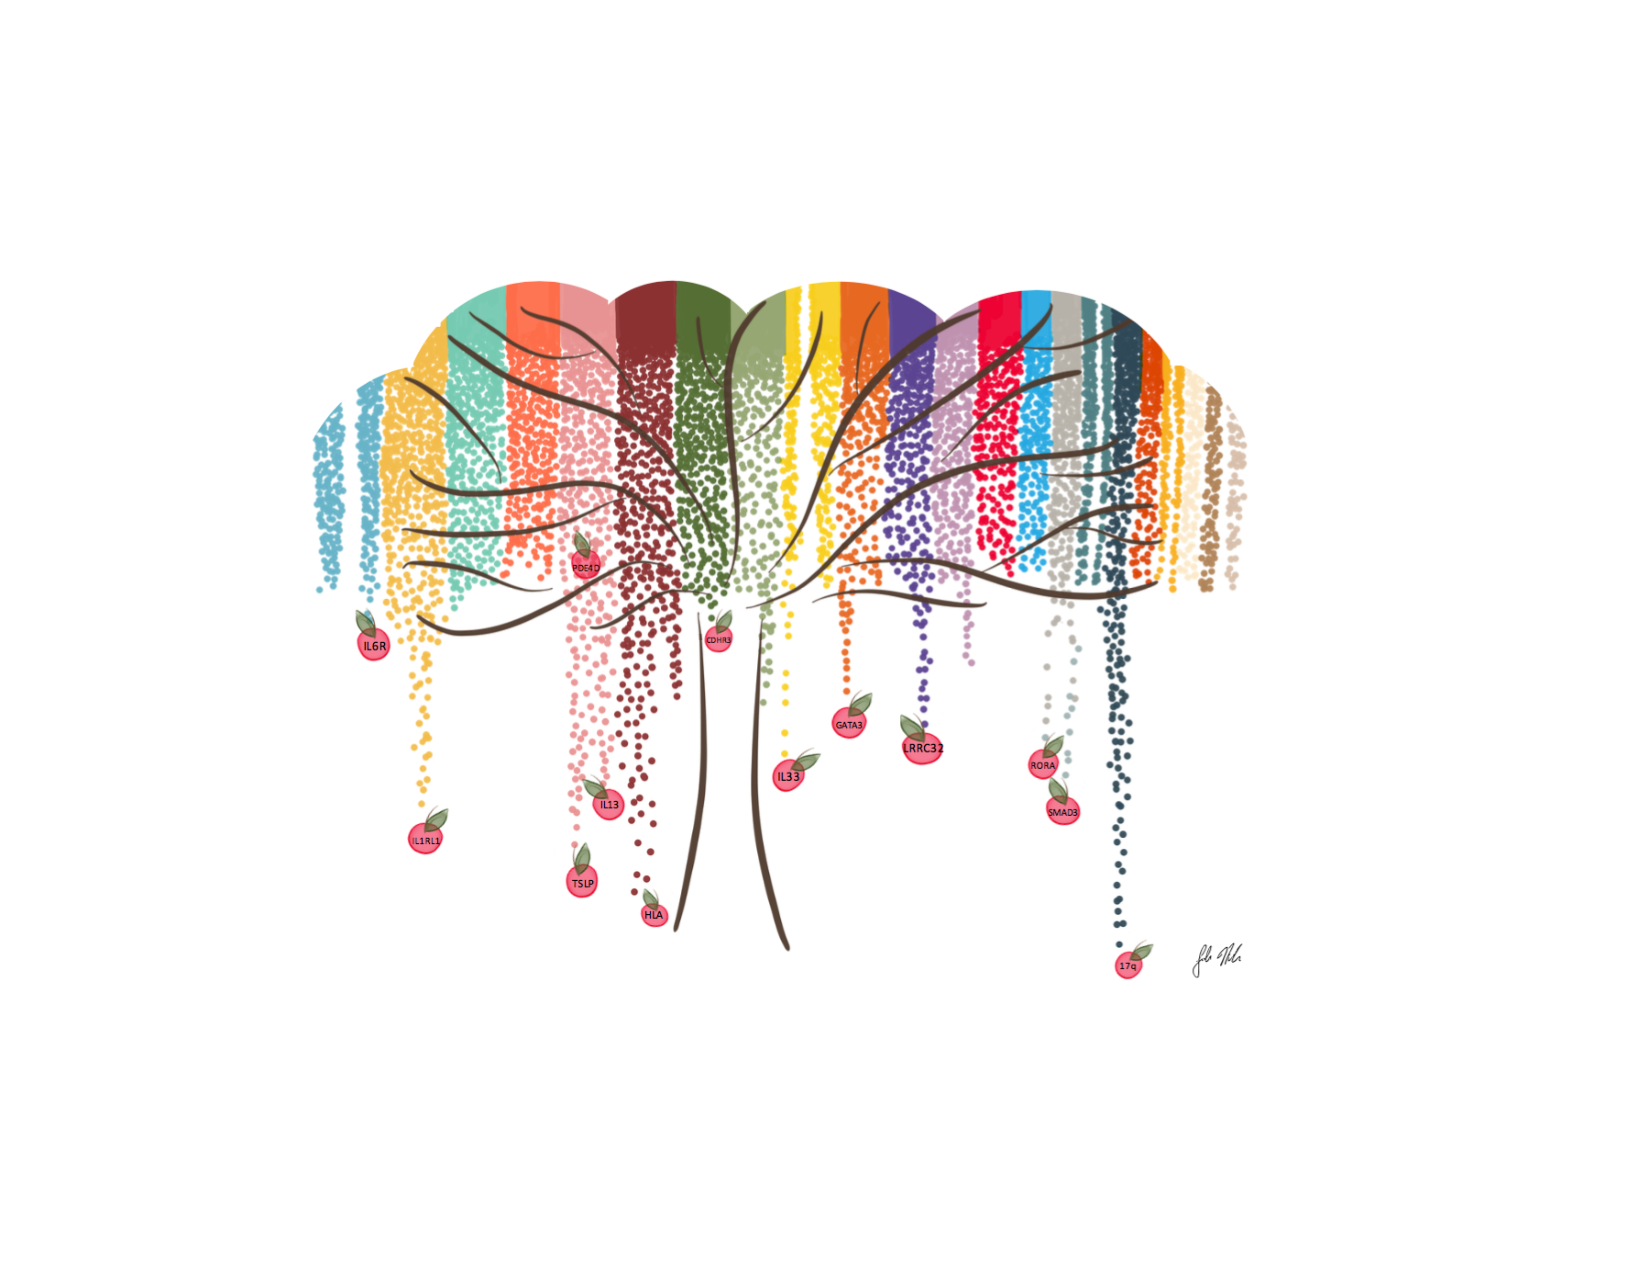
\includegraphics[width=8in]{img/ch01/fig-01-lowhangingfruit.pdf}
\caption[Low Hanging Fruit.]{\textbf{Asthma GWAS - low hanging fruit}}
\label{fig:lowhangingfruit}
\end{figure}


\section{The Origin of Genomic Imprinting }

Genomic imprinting in its broadest sense suggests that a phenotype observed for a particular gene or genes depends on the sex of the parent from with the gamete containing that gene or genes originated\cite{Sapienza:1989vm}. It was said that a particular gene is imprinted if it results in a different phenotype when it is maternally inherited versus paternally inherited.

The first use of the term "imprinting" was used in reference to the recognition by the cell of of chromosomes in \textit{Sciara}\cite{Crouse:1960vc,Sapienza:1989vm}. "The "imprint" a chromosome bears is unrelated to the genic constitution of the chromosome and is determined only by the sex of the germ line through with the chromosome has been inherited."\cite{Crouse:1960vc} 

The preferential inactivation of the paternally-derived X chromosomes in mouse were the first demonstrations of a functional imprint in mammalian genomes\cite{Takagi:1975ua,Lyon:1984gh,Chandra:1975tb}. The first suggestion of imprinting on autosomes was by a deletion on mouse chromosome 17 that showed a different phenotype based on which parent the deletion was inherited from.\cite{Johnson:1974uf,Johnson:1974kc}.

It was not until the development of the pronuclear transplantation technique that allowed for the creation of mice zygotes which contained only maternal or only paternal genetic contributions and provided evidence that the maternal and paternal genomes are not equal. The differential imprinting on the parental chromosomes prevented complete embryonic development in these mice with complete uniparental disomy.\cite{Sapienza:1989vm,McGrath:1984ky}.



\section{The Search for Parent of Origin Effects}




% Chapter 02
% Chapter 02
% !TEX encoding = UTF-8 Unicode
\chapter{Parent-of-Origin Effects on Quantitative Phenotypes in a Founder Population}\label{ch:pogwas}
\section[Abstract]{Abstract\footnotemark}


The impact of the parental origin of associated alleles in GWAS has been largely ignored. Yet sequence variants could affect traits differently depending on whether they are inherited from the mother or the father. To explore this possibility, we studied 21 quantitative phenotypes in a large Hutterite pedigree. We first identified variants with significant single parent (maternal-only or paternal-only) effects, and then used a novel statistical model to identify variants with opposite parental effects. Overall, we identified parent-of-origin effects (POEs) on 11 phenotypes, most of which are risk factors for cardiovascular disease. Many of the loci with POEs have features of imprinted regions and many of the variants with POE are associated with the expression of nearby genes. Overall, our results indicate that POEs, which can be opposite in direction, are relatively common in humans, have potentially important clinical effects, and will be missed in traditional GWAS. 


\footnotetext{Citation for chapter: Mozaffari SV, DeCara JM, Shah SJ, Lang RM, Nicolae DL, Ober C. Parent-of-Origin Effects on Quantitative Phenotypes in a Founder Population bioRxiv (2017). }

\section{Introduction}\label{ch02-introduction}
Genome-wide association studies (GWAS) typically treat alleles inherited from the mother and the father as equivalent, although variants can affect traits differently depending on whether they are maternal or paternal in origin. In particular, parent-of-origin effects (POEs) can result from imprinting, where epigenetic modifications allows for differential gene expression on homologous chromosomes that is determined by the parental origin of the chromosome. Mutations in imprinted genes or regions can result in diseases. For example, two very different diseases, Prader-Willi Syndrome (PWS) and Angelman Syndrome (AS), are due to loss of function alleles in genes within an imprinted region on chromosome 15q11-13. Inheriting a loss of function mutation for the \emph{SNRPN} gene from the father results in PWS but inheriting a loss of function mutation for the \emph{UBE3A} gene from the mother results in AS \citep{Peters2014,Falls1999}.  Long noncoding RNA genes at this and other imprinted regions act to silence (i.e.~ imprint) genes in cis. Imprinted genes are often part of imprinted gene networks, suggesting regulatory links between these genes \cite{Patten:2016cb,Gabory:2009be,Varrault:2006kn}. More than 150 imprinted loci have been described in humans \cite{Benonisdottir:2016dz} but there are likely many other, as yet undiscovered, imprinted loci. The kinship theory or conflict hypothesis suggests there is a conflict between the parent's interest on use of maternal resources by the fetus in utero. This theory promotes the idea that novel imprinted loci can affect more prominently phenotypes associated with fetal use of maternal resources, including early growth as well as downstream traits such as height, BMI, and metabolic disease \citep{Peters2014}.

Previous studies have utilized pedigrees to test maternal and paternal alleles separately for association with phenotypes or with gene expression to uncover new imprinted loci \citep{Kong:2009kk,Baran:2015cx,Garg2012a,Paper2014b,Benonisdottir:2016dz}. Kong \emph{et al} \citep{Kong:2009kk} discovered one locus associated with breast cancer risk only when the allele is inherited from the father and another locus associated with type 2 diabetes risk only when the allele is inherited from the mother. Garg et al. reported parent-of-origin cis-eQTLs with known or putative novel imprinted genes affecting gene expression \citep{Garg2012a}. Two additional studies by Zoledziewska et al. and Benonisdottir et al. identified opposite POEs on adult height at known imprinted loci \citep{Zoledziewska:2015do,Benonisdottir:2016dz}. Both studies reported associations with variants at the \emph{KCNQ1} gene, and one showed additional opposite POEs with height at two known imprinted loci (\emph{IGF2-H19} and \emph{DLK1-MEG3})\citep{Benonisdottir:2016dz}These studies provide proof-of-principle that alleles at imprinted loci can show POEs, some with opposite effects, with common phenotypes. 

Many existing studies and methods that identify POEs use case/parent trios or case/mother duos\citep{Chuang:2017kp,Howey:2012hj,Ainsworth:2010bp,Weinberg:1999km,Weinberg:1998cf}. Similar to Kong \emph{et al.} \citep{Kong:2009kk}, our method does not require data on the parent and only uses the parent-of-origin informative alleles which were assigned and phased using PRIMAL \citep{Livne2015}.  In contrast to Kong \emph{et al.} \citep{Kong:2009kk} which used binary traits, our method tests for POEs on quantitative traits, similar to Benonisdottir \emph{et al.} \citep{Benonisdottir:2016dz} which tested for POEs on height.

No previous study has included a broad range of human quantitative phenotypes or has studied genome-wide variants with effects in different directions depending on the parent of origin. To address this possibility, we developed a statistical model that directly compares the effects of the maternal and paternal alleles to identify effects that are different, including those that are opposite. We applied this model in a study of 21 common quantitative traits that were measured in the Hutterites, a founder population of European descent for which we have phased genotype data \citep{Livne2015}. We identified variants with maternally inherited or paternally inherited effects only and variants with opposite POEs. Some of the identified regions have characteristics similar to known imprinted genes. Overall, we show that this model can identify putative novel imprinted regions with POEs for a broad range of clinically relevant quantitative phenotypes.

\section{Results}\label{ch02-results}

\subsection{GWAS}\label{GWAS Results}
We first performed standard genome-wide association studies (GWAS) of 21 traits in the Hutterites (Table \ref{tab:tab-s1a}). These studies identified one genome wide significant association (p \textless $5 \times10^{-8} $) with each of five of the 21 traits: low density lipoprotein level (LDL)-cholesterol, triglycerides, carotid artery intima media thickness (CIMT), left ventricular mass index (LVMI), and monocyte count. The results of all 21 GWAS are summarized in Table \ref{tab:tab-s2} and Supplementary Figure \ref{fig:fig-s1a}. Results for all variants for all GWAS are deposited in dbGaP (phs000185 - submission in progress).

\subsection{Parent-of-Origin GWAS}\label{Parent-of-Origin GWAS}
We considered two possible mechanisms of POEs. In the first, the effect size of one parent's allele is close to zero and the effect size of the other parent's allele is significantly different from zero. For these cases, we performed a paternal only or maternal only GWAS. In other cases, the maternal and paternal alleles may both have effect sizes different from zero, but the effects are significantly different from each other or opposite in direction. To detect these types of POEs, we developed a model that tests for differences between parental effects (see Methods). This model is especially powerful to identify variants with parental effects in opposite directions.

\subsection{Maternal and Paternal GWAS}\label{Maternal and Paternal GWAS}
Using the same phenotypes, genotypes, pedigree, and criteria for significance as in the standard GWAS, we tested for maternal and paternal effects on each trait by testing each parentally inherited allele with the trait of interest, similar to previous studies \citep{Kong:2009kk,Zoledziewska:2015do,Garg2012a}. Variants were considered to have POEs if they had a p-value less than 5x10-8 in only one parent and were not significant in the standard GWAS (i.e., the LDL association on chromosome 19 and the triglycerides association chromosome 11 were not considered to have POEs; see Table \ref{tab:tab-s2}). The most significant parent-of-origin associations are summarized in Table \ref{tab:singleparent}. All significant results of the parent-of-origin GWAS for all 21 phenotypes are included in Table \ref{tab:tab-s5}. 


\begin{table}
\centering
\begin{adjustbox}{width={\textwidth}}
\begin{tabular}{@{}p{3cm}|p{2cm}p{2cm}p{2cm}p{2.5cm}p{1cm}p{0.5cm}p{1.5cm}p{2cm}p{2cm}p{2cm}@{}}
\toprule Phenotype & rsid & chr:loc & Variant Location & Nearest Gene & MAF & N & Beta (SE) & Paternal GWAS p-value & Maternal GWAS p-value & Standard GWAS p-value \\ \midrule
 \multicolumn{2}{c}{A. Maternal Associations} &&&&&&&&& \\ \hline
Age at Menarche  & rs7184983 (A/G) & 16:56554709 & Upstream & \emph{BBS2} & 0.059 & 336 & 0.862 (0.154) & 0.501 & 3.11E-08 & 6.75E-03 \\ \hline
CIMT  & rs4077567 (G/A) & 2:216703202 & Intronic & \emph{LINC00607}* & 0.30	& 429 & 0.047 (0.008) & 0.572 & 3.02E-08 & 4.21E-06 \\  \hline
\multirow{2}{3cm}{FEV\textsubscript{1}} & rs9849387 (A/G)	& 3:77764243 & Intergenic & \emph{ROBO2} & 0.39 & 1029 & -0.089 (0.015) & 0.387 & 4.10E-09 & 4.38E-04 \\ \cline{2-11}
 & rs6791779 (C/G) & 3:74996505 & Intergenic & \emph{MIR4444-1}* & 0.24 & 879 & -0.102 (0.021) & 0.069 & 1.48E-08 & 0.0452\\ \hline
LVMI & rs574232282 (G/A) & 1:41662388 & Intronic & \emph{SCMH1} & 0.018 & 537 & 0.239 (0.042) & 0.552 & 1.39E-08 & 1.05E-03\\ \hline
\multicolumn{2}{c}{B. Paternal Associations} &&&&&&&&&\\  \hline
\multirow{2}{3cm}{LDL} & rs12024326 (A/G) & 1:227146433 & Intronic & \emph{ADCK3} & 0.175 & 686 & -0.295 (0.048) & 8.06E-10 & 0.421 & 4.24E-05\\ \cline{2-11}
 & rs4843650 (A/G) & 16:87683486 & Intronic & \emph{JPH3} & 0.448 & 621 & 0.211 (0.036) & 6.57E-09 & 0.221 & 1.50E-04\\ \hline
SBP & rs1536182 (A/G) & 13:46275415 & Upstream & \emph{LINC01055}* & 0.2 & 684 & -0.028 (0.005)	& 1.53E-08 & 0.178 & 6.93E-04\\ \hline
Total cholesterol & rs113588203 (G/T) & 1:228979156 & Intergenic & \emph{RHOU} & 0.099 & 703 & -0.341 (0.060) & 1.76E-08 & 0.074 & 8.08E-03\\ \bottomrule
\end{tabular}
\end{adjustbox}
\caption[Phenotypes with significant single parent-of-origin associations. ]{\textbf{Phenotypes with significant single parent-of-origin associations.}
 *The most significant variant (P \textless $5 \times 10^{-8} $) at each locus for the (A) maternal and (B) paternal associations associated with each phenotype is shown. 
*non-coding RNA genes}
\label{tab:singleparent}
\end{table}


Overall, seven phenotypes had genome-wide significant parent-of-origin associations: four in the maternal only GWAS and three in the paternal only GWAS. Three cardiovascular disease (CVD)-associated phenotypes (age at menarche, CIMT, LVMI) and one lung function phenotype (forced expiratory volume in one second [FEV\textsubscript{1}]) were associated with maternally-inherited alleles only. 

When maternally inherited, the allele G at rs7184983 on chromosome 16 was associated with younger age of menarche (P = $ 3.11 \times 10^{-8}$) (Figure \ref{fig:menarche_mpgwas}). This SNP, rs7184983, is located upstream of the \emph{BBS2} gene and is associated with increased expression of \emph{OGFOD1} in transformed fibroblast cells and tibial nerve \cite{Consortium2015}. The maternally inherited G allele at rs4077567 on chromosome 2 was associated with decreased CIMT (P = $ 3.02 \times 10^{-8}$) (Figure \ref{fig:fig-s2}). This SNP is in the intron of a long intergenic noncoding gene, \emph{LINC00607}, that  is expressed in aorta, coronary, and tibial artery, all tissues potentially relevant to CIMT and atherosclerosis \cite{Consortium2015}. When maternally inherited, the allele G at rs574232282  in the intron of \emph{SCMH1} on chromosome 1 was associated with increased LVMI (P = $ 1.39 \times 10^{-8}$) (Supplementary Figure \ref{fig:fig-s3}). \emph{SCMH1} is expressed in aorta, coronary, and tibial artery \cite{Consortium2015}. \emph{SCMH1} protein associates with the polycomb group multiprotein complexes required to maintain the transcriptionally repressive state of certain genes \cite{Consortium2015}. Lastly, maternally inherited A allele at rs9849387 and maternally inherited C allele at rs6791779 on chromosome 3 were both associated with reduced FEV\textsubscript{1} (P = $ 4.10 \times 10^{-9}$ and $1.48 \times 10^{-8}$, respectively) (Supplementary Figure \ref{fig:fig-s4}). The nearest gene to rs9849387 is \emph{ROBO2} (65kb, downstream), which is expressed in the lung as well as in brain, and ovary \cite{Consortium2015}.The nearest gene to rs6791779 is \emph{MIR4444-1}(267kb) whose expression has not been characterized.

\begin{figure}[!htb]
\centering 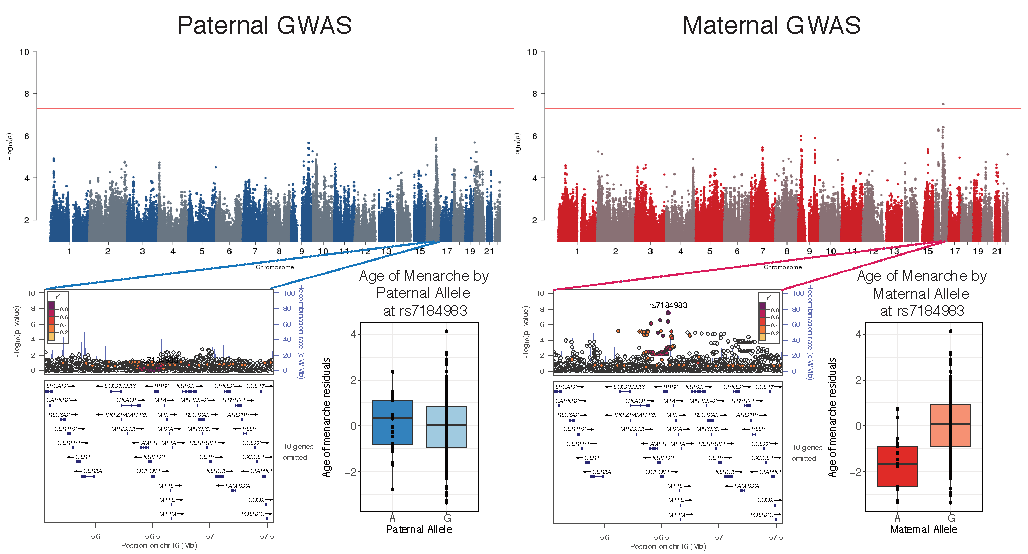
\includegraphics[width=6in]{img/ch02/fig-01-menarche_matpatgwas.pdf}
\caption[Maternal and Paternal GWAS results for Age of Menarche.]{\textbf{Maternal and Paternal GWAS results for Age of Menarche.}  The top panel shows the Manhattan plots from the paternal (left) and maternal (right) GWAS. LocusZoom plots for both GWAS are shown in the lower panel for the associated region in the GWAS. Boxplots show the distribution of age of menarche residuals (y-axes) by the corresponding maternal and paternal alleles at this SNP (x-axes). The horizontal bar of the boxplot shows the median, the box delineates the first and third quartile, and the whiskers show +/-1.5 x IQR.}
\label{fig:menarche_mpgwas}
\end{figure}

Three other CVD-related phenotypes (systolic blood pressure, LDL-C, and total cholesterol) had associations with paternally inherited alleles only. The paternally inherited A allele at rs12024326 on chromosome 1 was associated with lower LDL-cholesterol levels (P = $ 8.06 \times 10^{-10}$) (Figure \ref{fig:ldl_mpgwas}). rs12024326 is in the intron of gene \emph{ADCK3}, and the same allele was associated with increased expression of \emph{ADCK3} in whole blood, as well as decreased expression of a neighboring gene, \emph{CDC42BPA} in brain (cerebellum), heart (left ventricle), esophagus, and tibial artery \cite{Consortium2015}.When paternally inherited, the allele G at rs4843650 on chromosome 16 was associated with increased LDL-C and is located in the intron of \emph{JPH3}, which is expressed predominantly in the brain \cite{Consortium2015}. A SNP on chromosome 13 (rs1536182) was associated with systolic blood pressure levels when it was inherited from the father (Figure \ref{fig:fig-s5}). The paternally inherited A allele at this SNP was associated with decreased systolic blood pressure, as well as decreased expression of its closest gene, \emph{LINC01055}, a long intergenic noncoding gene, in testis \cite{Consortium2015}. A paternally inherited allele at rs113588203 (G) on chromosome 1 was associated with lower total cholesterol (P = $1.76 \times 10^{-8}$) (Figure \ref{fig:fig-s6}). This SNP is intergenic between \emph{RHOU} (96kb, downstream), which is expressed across multiple tissues, and \emph{MIRR4454} (331kb), which is expressed in adipose, kidney and heart tissues \cite{Consortium2015}. 


\begin{figure}[!htb]
\centering 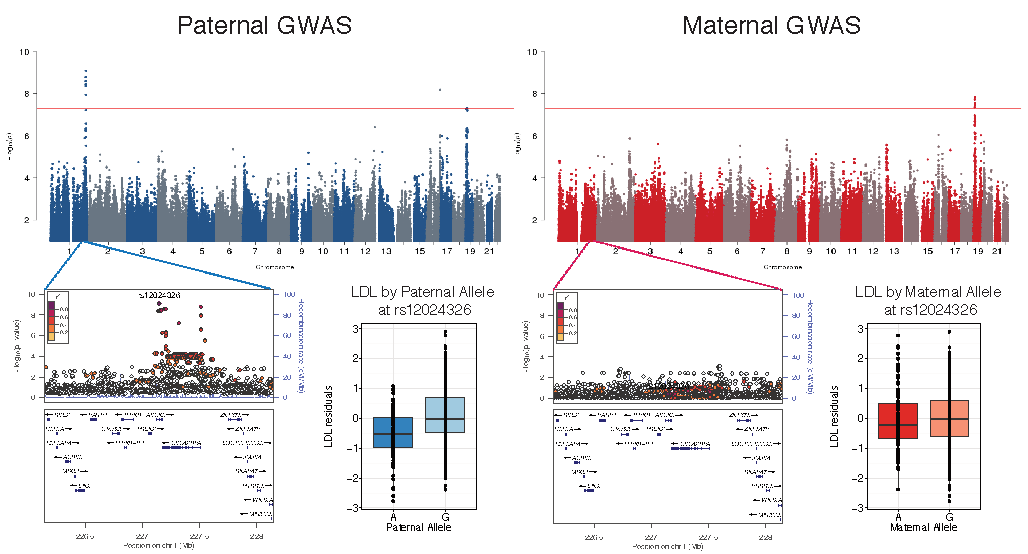
\includegraphics[width=6in]{img/ch02/fig-02-ldl_matpatgwas.pdf}
\caption[Maternal and Paternal GWAS results for LDL Cholesterol.]{\textbf{Maternal and Paternal GWAS results for LDL Cholesterol.}  The top panel shows the Manhattan plots from the paternal (left) and maternal (right) GWAS. LocusZoom plots for both GWAS are shown in the lower panel for the associated region in the GWAS. Boxplots show the distribution of LDL residuals (y-axes) by the corresponding maternal and paternal alleles at this SNP (x-axes). The horizontal bar of the boxplot shows the median, the box delineates the first and third quartile, and the whiskers show +/-1.5 x IQR.}
\label{fig:ldl_mpgwas}
\end{figure}


\subsection{GWAS for Differential Parent-of-Origin Effects}\label{GWAS for Differential Parent-of-Origin Effects}

Because some imprinted regions include genes that have both maternal or paternal specific tissue expression, we next tested for such differential effects with these 21 phenotypes. In these analyses, we compared the effect and direction of the association between maternal and paternal alleles to identify variants that have different effects, including opposite effects, on the phenotype. Such loci would be completely hidden in standard GWAS in which paternally and maternally inherited alleles are combined. These opposite effect GWAS revealed 11 independent loci with opposite POEs for nine different traits, at least six of which are associated with CVD risk (Table \ref{tab:oppparent}, Figure \ref{fig:fig-s7}). 


\begin{table}
\centering
\begin{adjustbox}{width={\textwidth}}
\begin{tabular}{@{}p{3cm}|p{1.8cm}p{2cm}p{2cm}p{2cm}p{0.8cm}p{1.8cm}p{2.5cm}|p{1.8cm}p{1.8cm}|p{1.8cm}p{1.8cm}|p{1.8cm}@{}}
\toprule \multirow{2}{3cm}{Phenotype} & \multirow{2}{1.8cm}{rsid} & \multirow{2}{2cm}{chr:loc} & \multirow{2}{2cm}{Variant Location} & \multirow{2}{2cm}{Nearest Gene} 
& \multirow{2}{0.8cm}{MAF} & \multirow{2}{1.8cm}{$\beta_{M}-\beta_{P}$ (SE) }& \multirow{2}{2.5cm}{Opposite Effect GWAS} & \multicolumn{2}{c}{Paternal GWAS} & \multicolumn{2}{c}{Maternal GWAS} & \multirow{2}{1.8cm}{GWAS p-value}\\ \cline{9-12}
&&&&&&& & P-value & Beta(SE) & P-value & Beta(SE) &  \\ \midrule
Age of menarche & rs12447191 & 16:62199299 & Intergenic & \emph{CDH8} & 0.17	  & -0.654 (0.109)	& 5.27E-09	& 5.20E-06&	0.391 (0.085)	& 1.85E-05 & -0.368 (0.085)& 	0.868\\ \hline
\multirow{2}{3cm}{BMI}& rs77785972 & 5:97415767 & Intergenic & \emph{LINC01340}* & 0.025 & 0.154 (0.025) & 5.12E-10 & 5.84E-07	 & -0.094 (0.019) & 1.58E-05 &  0.081 (0.019) & 0.539\\ \cline{2-13}
&  rs17605739 & 6:22962798 & Intronic &  \emph{RP1-209A6.1}* & 0.17 & 0.053 (0.010) & 3.01E-08 & 6.99E-05 & -0.032 (0.008) & 1.42E-06 & 0.034 (0.007) & 0.156\\ \hline
Eosinophil count & rs2355879 & 1:18732860 & Intergenic & \emph{IGSF21} & 0.14 & 0.091 (0.016) & 1.69E-08 & 5.83E-08  & -0.065 (0.012) & 5.59E-04 & 0.043 (0.012) & 0.253 \\ \hline
FEV1 & rs12714812 & 3:74813002 & Intergenic & \emph{CNTN3} & 0.45 & -0.119 (0.021) & 4.52E-08 & 1.78E-03 & 0.052 (0.017) & 6.35E-06 & -0.073 (0.016) & 0.958\\ \hline
LDL & rs1032596 & 16:86281537 & Intronic & \emph{LINC01081}* & 0.30 & -0.310 (0.056) & 3.69E-08 & 1.05E-06 & 0.201 (0.041) & 4.56E-04 & -0.148 (0.042) & 0.271\\ \hline
LVMI	 & rs16853098 & 2:168013281 & Intronic & \emph{XIRP2} & 0.12 & -0.091 (0.053) & 4.18E-08 & 5.29E-06 & 0.064 (0.014) & 2.04E-04 & -0.048 (0.013) & 0.926\\ \hline
Neutrophil count & rs142030841 & 18:34371947 & Intronic & \emph{TPGS2} & 0.042 & -0.224 (0.041)	 & 4.40E-08 & 2.25E-03 & 0.078 (0.025) & 1.30E-07 & -0.188 (0.035) & 0.577\\ \hline
Triglycerides & rs7525463 & 1:218860879 & Intronic & \emph{MIR548F3}* & 0.16 & -0.401 (0.071) & 2.51E-08 & 1.14E-03 & 0.195 (0.060)  & 5.52E-08 & -0.267 (0.049)	& 0.028\\ \hline
Total cholesterol & rs7033776 & 9:36704465 & Intergenic & \emph{MELK} & 0.41 & 0.230 (0.041) & 4.12E-08 & 5.60E-08	& -0.183 (0.034) & 2.28-03 & 0.099 (0.032) & 0.067\\ \hline
\bottomrule
\end{tabular}
\end{adjustbox}
\caption[Significant Opposite Parent-of-Origin Effect GWAS Associations.]{\textbf{Significant Opposite Parent-of-Origin Effect GWAS Associations.} The most significant variant at each locus for each phenotype is shown.  $\beta_{M}-\beta_{P}$ represents difference in parental effect size.
*non-coding RNA genes
}
\label{tab:oppparent}
\end{table}




A locus on chromosome 16, near the \emph{CDH8} gene (128kb, upstream), was associated with opposite POEs with age of menarche (Figure \ref{fig:menarche_oegwas}). \emph{CDH8} is highly expressed in the brain, as well as in the aorta artery and pituitary gland. Two loci on chromosomes 5 and 6 were associated with opposite POEs on body mass index (BMI) (Figure \ref{fig:bmi_oegwas}). The most significant variant on chromosome 5 (rs77785972) is near a long intergenic noncoding gene, \emph{LINC01340} (409kb, downstream), whose expression has not been well characterized. The SNP on chromosome 6 (rs17605739) is also in a long intergenic noncoding gene, \emph{RP1-209A6.1}, which is expressed in low levels in the tibial artery, bladder, spleen, lung, pituitary gland, as well as testis. 


\begin{figure}[!htb]
\centering 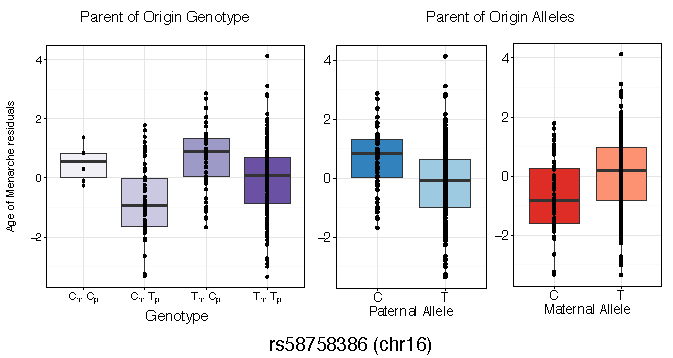
\includegraphics[width=5in]{img/ch02/fig-03-menarche_oegwas.pdf}
\caption[Opposite Effect Parent-of-Origin GWAS Result for Age of Menarche.]{\textbf{Opposite Effect Parent-of-Origin GWAS Result for Age of Menarche.}  Box plots of age of menarche residuals (y-axes) are shown for each of the four genotypes (left panel; x-axis), and for paternal (center panel; x-axis) and maternal (right panel; x-axis) alleles. The maternal C allele is associated with decreased and maternal T allele with increased age of menarche. The paternal C allele is associated with increased and the paternal T allele with decreased age of menarche. The horizontal bar of the boxplot shows the median, the box delineates the first and third quartile, and the whiskers show +/-1.5 x IQR.}
\label{fig:menarche_oegwas}
\end{figure}

\begin{figure}[!htb]
\centering 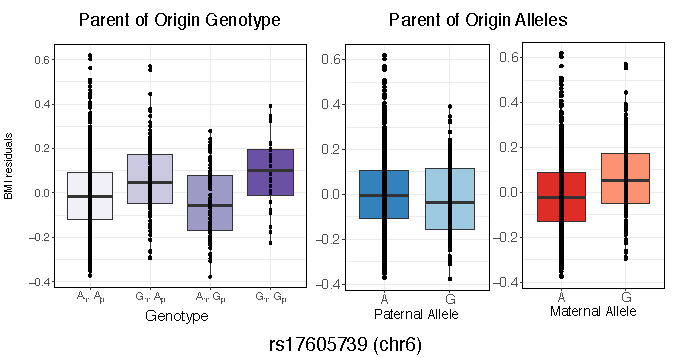
\includegraphics[width=5in]{img/ch02/fig-04-bmi_oegwas.pdf}
\caption[Opposite Effect Parent-of-Origin GWAS Result for BMI.]{\textbf{Opposite Effect Parent-of-Origin GWAS Result for BMI.}  Box plots of two significant loci plot BMI residuals (y-axes) for each of the four genotypes (left panel; x-axis), and for paternal (center panel; x-axis) and maternal (right panel; x-axis) alleles. For the (A) SNP on chromosome 5 the maternal A allele is associated with decreased and maternal G allele with increased BMI. The paternal A allele is associated with increased and the paternal G allele with decreased BMI. For the (B) SNP on chromosome 6 the maternal A allele is associated with decreased and maternal G allele with increased BMI. The paternal A allele is associated with increased and the paternal G allele with decreased BMI. The horizontal bar of the boxplot shows the median, the box delineates the first and third quartile, and the whiskers show +/-1.5 x IQR.}
\label{fig:bmi_oegwas}
\end{figure}



 A SNP on chromosome 16 (rs1032596) was associated with opposite POEs on LDL-cholesterol (Figure \ref{fig:fig-s8}). This SNP lies in the intron of another long noncoding RNA gene, \emph{LINC01081}, which has been suggested to be imprinted because its downstream genes have also been shown to have parent- and tissue-specific activity \cite{Szafranski:2016fz}. A region on chromosome 2 has opposite effects associated with LVMI (Figure \ref{fig:fig-s9}). The associated SNPs are in the intron of \emph{XIRP2}, a cardiomyopathy associated protein that is expressed in skeletal muscle and heart left ventricle, suggesting that this gene could play a role in determining left ventricular mass \cite{Wang:2014jg,Nilsson:2013jy,Consortium2015}. In addition, the most significant SNP at this region, rs17616252 (and multiple SNPs in LD) is a strong eQTL (P = $1.8 \times10^{-13} $) for the gene \emph{XIRP2} in skeletal muscle, \emph{XIRP2-AS1} in testis, and \emph{B3GALT1} in transformed fibroblast cells \cite{Consortium2015}. Four variants in a region on chromosome 1 in a microRNA gene, \emph{MIR548F3}, were associated with opposite POEs on triglyceride levels (Figure \ref{fig:fig-s10}). The expression of \emph{MIR548F3} has not been characterized. SNP rs7033776 near \emph{MELK} (27kb, downstream) on chromosome 9 was associated with opposite effects on total cholesterol (Figure \ref{fig:fig-s11}). \emph{MELK} is expressed in the colon and esophagus in addition to transformed lymphocytes and fibroblasts \cite{Consortium2015}. 


Nine linked variants on chromosome 1 were associated with opposite POEs of blood eosinophil count (Figure \ref{fig:fig-s12}). These variants are near the gene \emph{IGSF21} (27kb, downstream) which is a member of the immunoglobulin superfamily and likely acts as a receptor in immune response pathways \cite{OLeary:2016cm}. A variant on chromosome 3, rs12714812, was associated with opposite POEs for FEV\textsubscript{1} (Figure \ref{fig:fig-s13}). This variant has been shown to regulate the expression of a gene \emph{CNTN3} (45kb, upstream) in heart and brain \cite{Consortium2015}. Studies in mice have suggested that this gene is imprinted and maternally expressed in the murine placenta \cite{Brideau:2010gz}. Variant rs142030841 in the intron of the gene \emph{TPGS2} on chromosome 18 has opposite POEs with neutrophil levels (Figure \ref{fig:fig-s14}). This SNP is an expression quantitative trait locus (eQTL) for the noncoding RNA gene \emph{RP11-95O2.5} in skin, testis, breast, thyroid and adipose tissue, for \emph{CELF4} in tibial nerve and lung, and for \emph{TPGS2} in tibial artery and transformed fibroblast cells \cite{Consortium2015}.


\subsection{Parent-of-Origin Effects on Gene Expression}\label{Parent-of-Origin Effects on Gene Expression}

To determine if any of the associated variants also showed POEs on gene expression in the Hutterites, we used RNA-seq gene expression data from lymphoblastoid cell lines (LCLs) collected from 430 of the individuals in the GWAS sample. We first tested for association of maternal and paternal variants with genes detected as expressed in the LCLs and whose transcript start site was within 1Mb of each associated SNP. There were no significant associations after multiple testing correction, similar to a previous study \cite{Benonisdottir:2016dz}. However, because we considered this to be exploratory analyses, we show results for the five most significant parent-of-origin eQTLs (Table \ref{tab:pogexp}). We next used the opposite effect model for each SNP in Table \ref{tab:oppparent} and expression of all genes that were detected as expressed in LCLs and whose transcript start site was within 1Mb of the associated SNP. This resulted in 57 tests (1 SNP for each of 8 phenotypes, and 57 genes). The five most significant opposite effect eQTLs, none of which passed the Bonferroni threshold of 8.77 x 10-4, are shown in Table \ref{tab:oppgexp}. The most significant opposite effect eQTL was for \emph{POLR1E} expression with the SNP on chromosome 9 (rs7033776) that was associated with total cholesterol (opposite effect eQTL P = $9.86 \times10^{-4} $) (Figure \ref{fig:fig-s15}). \emph{POLR1E} is involved in the purine metabolism pathway as well as DNA-directed polymerase activity. The same SNP, rs7033776, had modest opposite effects with the expression of three other genes in the region (\emph{PAX5}, \emph{FBXO10}, and \emph{FRMPD1}), a signature consistent with an imprinted region. Another SNP with opposite POEs on LVMI, rs16853098, was an opposite effect eQTL for \emph{STK39}, a gene that has been previously associated with hypertension \cite{Wang:2009bt}.



\begin{table}
\centering
\begin{adjustbox}{width={\textwidth}}
\begin{tabular}{@{}p{3cm}|p{2cm}p{2cm}p{2cm}p{2.5cm}p{2cm}p{2cm}p{2cm}@{}}
\toprule Phenotype & Sample Size & rsid & chr:loc & Gene & Beta (SE) & Maternal eQTL p-value & Paternal eQTL p-value  \\ \midrule
 \multicolumn{2}{c}{A. Maternal Associations} &&&&&& \\ \hline

CIMT & 334 & rs4077567 & 1:216703202 & \emph{ABCA12} & 0.039 (0.017) & 0.0214 & 0.0153 \\ \hline
Age at menarche & 336 & rs7184983 & 16:56554709 & \emph{POLR2C} & -0.085 (0.039) & 0.0291 & 0.793 \\ \hline
Age at menarche & 336 & rs7184983 & 16:56554709 & \emph{SLC12A3} & -0.064 (0.031) & 0.0377 & 	0.228 \\ \hline
CIMT & 334 & rs4077567 & 1:216703202 & \emph{RPL37A} & 0.030 (0.016) & 0.0572 & 0.590 \\ \hline
LVM & 457 & rs74232282 & 1:41662388 & \emph{SMAP2} & 1.40 (0.159) & 0.0582	& 0.112 \\ \hline
 \multicolumn{2}{c}{B. Paternal Associations} &&&&&&  \\ \hline
Total cholesterol & 352 & rs113588203 & 1:228979165 & \emph{HIST3H2A} & 	0.560 (0.308) & 	0.881 & 	0.0685 \\ \hline
Total cholesterol & 352 & rs113588203 & 1:228979165 & \emph{SPHAR} & 	0.073 (0.047) & 	0.601 & 	0.120 \\ \hline
LDL & 352 & rs1110603 & 16:87687317 & \emph{MAP1LC3B} & -0.024 (0.015) & 	0.435 & 	0.125 \\ \hline
LDL & 352 & rs1110603 & 16:87687317 & \emph{FBXO31} & -0.027 (0.018)	 & 0.156 & 	0.136 \\ \hline
Total cholesterol & 357 & rs113588203 & 1:228979165 & \emph{RAB4A} & 	-0.039 (0.028) & 	0.616 & 	0.159\\ \bottomrule
\end{tabular}
\end{adjustbox}
\caption[Parent-of-Origin eQTLs in LCLs. ]{\textbf{Parent-of-Origin eQTLs in LCLs.}The most significant SNP for each phenotype (Table \ref{tab:singleparent}) was tested for association with gene expression for genes with TSS within 1Mb of the SNP. The effect sizes correspond to the maternal (A) or paternal (B) effect sizes.}
\label{tab:pogexp}
\end{table}



\begin{table}
\centering
\begin{adjustbox}{width={\textwidth}}
\begin{tabular}{@{}p{3cm}|p{2cm}p{2cm}p{2cm}p{2.5cm}p{2cm}p{2cm}@{}}
\toprule Phenotype & Sample Size & rsid & chr:loc & Gene & $\beta_{M}-\beta_{P}$ (SE) & Opposite Effect p-value  \\ \midrule
Total cholesterol & 381 & rs7033776	 & 9:36704465	 &\emph{POLR1E} & 	0.0603 (0.399) & 9.86E-04\\ \hline
Total cholesterol & 381 & rs7033776	 & 9:36704465	 &\emph{PAX5} & 	0.0608 (0.0253) & 	0.0162\\ \hline
Total cholesterol & 381 & rs7033776	 & 9:36704465	 &\emph{FBXO10} & 	0.0789 (0.0337) & 	0.019\\ \hline
LVMI	 & 355 & rs16853098 & 2:168013281 	 & \emph{STK39}	 &-0.238 (0.124) & 	0.055\\ \hline
Total cholesterol & 381 & rs7033776 & 	9:36704465 & 	\emph{FRMPD1} & 	0.185 (0.0988) & 	0.060 \\ \bottomrule
\end{tabular}
\end{adjustbox}
\caption[Opposite Parent-of-Origin eQTLs in LCLs. ]{\textbf{Opposite Parent-of-Origin eQTLs in LCLs.} The most significant SNP for each phenotype (Table \ref{tab:oppparent}) was tested for opposite effect eQTLs with genes with TSS within 1Mb of the SNP. The effect size corresponds to the difference in maternal and paternal effect sizes.}
\label{tab:oppgexp}
\end{table}



\section{Discussion}\label{ch02-discussion}

In this study, we introduced a novel statistical method that allows assessment of standard GWAS signals along with measures of differential POEs on common quantitative phenotypes. Similar to previous parent-of-origin studies of fewer phenotypes \cite{Kong:2009kk,Benonisdottir:2016dz,Garg2012a}, we tested for associations of maternally- or paternally-derived alleles with each phenotype. We then extended this method to identify variants for which maternally- and paternally-derived alleles have different, including opposite, effects on phenotypic values. The focus on 21 common disease-associated phenotypes in a single large pedigree allowed us to broadly survey physiological effects of putative imprinted regions and the candidate genes at each associated locus. In contrast to previous studies, our new model can identify variants with opposite POEs that would be missed in traditional GWAS (Table \ref{tab:oppparent}). 

Our studies of \textgreater1,000 Hutterites who are related to each other in a single pedigree allowed us to detect POEs, even when few genome-wide significant associations were detected in standard GWAS of the same phenotypes. Our method revealed parent-of-origin specific genome-wide significant associations for seven of the 21 phenotypes examined, with maternally-inherited alleles associated with four phenotypes, paternally-inherited alleles with three phenotypes (Table \ref{tab:singleparent}), and opposite parent-of-origin alleles with nine phenotypes, of which five also showed single POEs at different loci (Table \ref{tab:oppparent}). Overall, 11 of the 21 phenotypes examined showed genome-wide significant evidence of POEs with alleles at one or more loci. In contrast, standard GWAS of these same phenotypes and using the same markers in these same individuals revealed genome-wide significant association for only five traits. 

It is notable that four of the nine significant opposite POEs (one each with LDL-C and triglycerides, and two with BMI) lie in or near long intergenic non-coding RNA genes (lincRNAs). LincRNAs are a feature of imprinted regions \cite{Peters2014}, where they can silence the expression of genes on the opposite chromosome \cite{Barlow:2014dv,Patten:2016cb}. One of the variants, rs1032596, with an opposite parent-of-origin effect on LDL-C is located in the \emph{LINC01081} gene. This noncoding RNA, along with \emph{LINC01082}, regulates the \emph{FOXF1} enhancer resulting in \emph{FOXF1} parent- and tissue-specific activity\cite{Szafranski:2016fz} providing experimental support for tissue specific expression, a feature of imprinted regions. 

Another variant with POEs in our study has been suggested to be imprinted in previously published work. The variant associated with opposite POEs for FEV\textsubscript{1} is an eQTL for the gene \emph{CNTN3}. \emph{CNTN3} was shown to have exclusive maternal allele-specific expression in murine placentas\cite{Brideau:2010gz}, although this finding may have been due to contaminating maternal cells \cite{Okae:2011hj,Proudhon:2011eh}. 

Other regions associated with POEs harbor genes involved in transcriptional repression (e.g., \emph{SCMH1} with LVMI on chromosome 1) or the associated SNPs are reported as eQTLs in GTEx with expression in tissues relevant to the phenotype under investigation (e.g., the LVMI-associated SNPs are eQTLs for \emph{XIRP2}, which is expressed in skeletal muscle and heart left ventricle) \cite{Consortium2015}. Overall, these patterns of expression provide additional support that the parent-of-origin associations in our study are flagging imprinted regions or regions involved in the regulation of gene expression. Finally, we used gene expression in LCLs from the Hutterites to directly test for parent-of-origin eQTLs among SNPs associated with phenotypes in the parent-of-origin GWAS. Although none of the parent-of-origin eQTLs met criteria for significance after correcting for multiple testing, the SNP on chromosome 9 with opposite POEs on total cholesterol levels was borderline significant as an opposite parent-of-origin eQTL for \emph{POLR1E}, and possible for three other genes at the same locus (\emph{PAX5}, \emph{FBXO10}, and \emph{FRMPD1}). The presence of multiple genes with potential parent-of-origin expression patterns is further supportive of an imprinted locus. The availability of gene expression only in LCLs from the Hutterites limits the inferences we can draw about effects on expression because imprinted regions are often tissue-specific and sometimes developmentally regulated \cite{Peters2014,Falls1999}. Despite this limitation, the fact that many of the SNPs associated with POEs on phenotypes are themselves eQTLs in relevant tissues (GTEx) and some are suggestive of having POEs on expression in LCLs from the Hutterites is generally supportive of the suggestion that some of the regions identified in this study are imprinted or have network interactions with imprinted genes\cite{Chess:2016fs} in humans. Additionally, our data suggest that loci with POEs influence a broad spectrum of quantitative phenotypes that are themselves risk factors for common diseases. 

 In particular, the discovery of POEs for eight traits that are associated with cardiovascular disease risk is intriguing. These include metabolic phenotypes, such as BMI, total cholesterol, triglycerides, LDL, and age of menarche, that have indirect effects on cardiac health, as well as LVMI and CIMT, which more directly reflect cardiac health. Some of these phenotypes showed associations with paternally inherited alleles only (systolic blood pressure, LDL-C, total cholesterol), maternally inherited alleles only (LVMI, CIMT, and age at menarche), and/or with opposite effect variants (BMI, LDL-C, triglycerides, total cholesterol, LVMI, age at menarche). It has been suggested that genomic imprinting evolved in the mammalian lineage as a way to regulate maternally and paternally expressed genes in the placenta during pregnancy and modulate metabolic functions related to growth, where the parental interests may be in conflict — paternal alleles favoring growth of the fetus at the expense of the mother while maternal alleles favor restricting resources to the fetus to ensure preservation of her nutritional needs \cite{Haig:2000if,Barlow:2014dv,Patten:2016cb}. Our data show some effects that are consistent with this theory. For example, three independent paternally inherited alleles on chromosome 1 are associated with increased LDL-C (Fig. 2) and total cholesterol (Figure \label{fig:fig-s7}); a paternal allele on chromosome 13 is also associated with increased systolic blood pressure (Figure \label{fig:fig-s6}). However, it is not always possible to interpret our results in light of this model, such as the association of maternal allele on chromosome 2 with decreased CIMT (Figure \ref{fig:fig-s3}), or the maternal allele on chromosome 16 associated with decreased age of menarche (Figure  \ref{fig:menarche_mpgwas}), which confers increased cardiovascular risk \cite{Canoy:2015ha}. However, because many of the traits associated with POEs in this study were measured in adults, and none were measured in neonates, we are likely observing the downstream effects of processes that occurred in utero. Nonetheless, this kinship theory, or parent-conflict hypothesis, could account for the enrichment of parent-of-origin associations, particularly those with opposite effects, among metabolic and CVD-associated traits \cite{Peters2014}.
 
 Finally, we note that the parent-of-origin GWAS for 21 phenotypes in the Hutterites revealed overall twice as many genome-wide significant loci compared to standard GWAS of the same phenotypes in the same individuals, suggesting that variation at imprinted loci may represent some of the "missing heritability" of these phenotypes and potentially for the disease for which they confer risk. This idea is consistent with observations in both mice and humans \cite{Laurin:2017jv}. POEs in mice contribute disproportionally to the heritability of 97 traits, including those related to total cholesterol, weight, HDL, and triglycerides \cite{Mott2014}. Exactly how much loci with POEs in humans contribute to phenotypic variation and disease risk overall remains to be determined, but our study provides compelling evidence that it is likely to be significant for many important traits.


\section{Methods}\label{ch02-methods}

\subsection{Sample Composition}\label{Sample Composition}
The individuals in this study have participated in one or more of our studies on the genetics of complex traits in the Hutterites \cite{Cusanovich:2016id,Weiss:2005cq,Abney2001}. The more than 1,500 Hutterites in our study are related to each other in a 13-generation pedigree including 3,671 individuals. 

\subsection{Genotype Data}\label{Genotype Data}
Variants detected in the whole genome sequences of 98 Hutterites were previously imputed to an additional 1,317 individuals using PRIMAL, a high-accuracy pedigree based imputation method \cite{Livne2015}. PRIMAL was used to phase alleles and assign parent of origin for 83\% of about 12 million autosomal SNPs. For these studies, we selected SNPs that had a MAF 1\% and genotype call rate 85\%. This yielded 5,891,982 autosomal SNPs. Parent-of-origin allele call rates differed among individuals and between phenotypes (Table \ref{tab:tab-s1a}).

\subsection{Phenotype Data}\label{Phenotype Data}
We included 21 quantitative phenotypes that were previously measured in the Hutterites. Descriptions for each phenotype, as well as exclusion criteria, transformations, and covariates used with each phenotype in the GWAS, are available in the Supplementary Methods (Table \ref{tab:tab-s1a}). 

Descriptions for 18 of the 21 phenotypes can be found in Cusanovich et al \cite{Cusanovich:2016id}. The remaining three are described here. Height was measured in cm on a stadiometer with shoes removed. BMI was calculated using weight (kg, measured on scale) divided by height (m) squared. Age at menarche was collected retrospectively by interview. 

\subsection{GWAS}\label{GWAS Methods}
We used a linear mixed model as implemented in GEMMA to test for genome wide association with 21 phenotypes using an additive model. We corrected for relatedness, as well as relevant covariates (Table \ref{tab:tab-s1a}).


\subsection{Maternal and Paternal GWAS}\label{Maternal and Paternal GWAS Methods}
To evaluated the evidence for POEs, we tested maternal and paternal alleles separately with each phenotype, comparing phenotypic differences between the maternally inherited alleles and between the paternally inherited alleles. We used a linear mixed model as implemented in GEMMA, which allows us to correct for relatedness as a random effect, as well as sex, age, and other covariates as fixed effects \cite{Zhou2012}.The linear mixed model for the parent-of-origin GWAS for testing maternal alleles and paternal alleles is shown in Equation 2.1 and Equation 2.2, respectively. 

\begin{equation}
Y =W\alpha + X_{M}\beta_{M}+g+\epsilon
\end{equation}

\begin{equation}
Y =W\alpha + X_{P}\beta_{P}+g+\epsilon
\end{equation}

$n$ is the number of individuals, $Y$ is an $n \times 1$ vector of quantitative traits, $W$ is an $n \times c$ matrix of covariates (fixed effects) including intercept 1. $\alpha$ is a $c \times 1$ vector of covariate coefficients. $X_M$  is an $n \times 1$ vector of maternal alleles, and $X_P$ an $n \times 1$ vector of paternal alleles. $\beta_M$ and $\beta_P$ are the effect sizes of maternal and paternal alleles, respectively. g is a vector of genetic effects with $g \sim N(0, A(\sigma_g)^2 )$ where A is the genetic relatedness matrix; $\epsilon$ is a vector of non-genetic effects with $\epsilon \sim N(0,I(\sigma_e)^2)$.

\subsection{Differential Effect GWAS (PO-GWAS)}\label{Differential Effect GWAS (PO-GWAS)}
To test for a difference in the same allele inherited from each parent, including opposite effects, we re-parameterized the test model (Equation 2.3) from Garg et al \cite{Garg2012a}. The null model (Equation 2.4) is a standard GWAS model, ignoring parent of origin of alleles. The test model (Equation 2.3) is more significant when maternal and paternal alleles have differential effects on gene expression.

\begin{equation}
Y =W\alpha + X_{M}\beta_{M}+ X_{P}\beta_{P}+g+\epsilon
\end{equation}

\begin{equation}
Y =W\alpha + X_{MP}\beta_{MP}+g+\epsilon
\end{equation}

This new model allows us to measure the difference in parental effect of the same allele when the genotype is a covariate in Equation 2.5. 
\begin{equation}
Y =W\alpha + \frac{X_{M}-X_{P}}{2}(\beta_{M}-\beta_{P}) + X_{MP}\frac{(\beta_{P}+\beta_{M})}{2} +g+\epsilon
\end{equation}

$X_{MP}$ is a $n \times 1$ vector of genotypes with possible values [ 0,1,2 ], equivalent to $X_P+ X_M. (\beta_M-\beta_P )$ is the difference in parental effect size. If the difference in parental effect size is large and significantly different from 0 it suggests a parent-of-origin effect exists at this variant. $((X_M-X_P ))/2$ is a $n \times 1$ vector of genotypes with possible values [-1,0,1].  $((\beta_P+\beta_M))/2$   is the average parental effect size that is captured in normal GWAS using genotypes. The average genotypes are added in as a covariate, with the average parental effect size the corresponding covariate coefficient. This differential effect GWAS was implemented in GEMMA using BIMBAM format to use average genotype values \cite{Servin:2007gj}.


\subsection{Parent-of-Origin eQTL studies}\label{Parent-of-Origin eQTL studies}

RNA-seq data from LCLs were available from a previous study in the Hutterites \cite{Cusanovich:2016id}. For this study, sequencing reads were reprocessed as follows. Reads were trimmed for adaptors using Cutadapt (with reads \textless5 bp discarded) then remapped to hg19 using STAR indexed with gencode version 19 gene annotations \cite{Dobin:2002by,Martin:2011eu}. To remove mapping bias, reads were processed using the WASP mapping pipeline \cite{vandeGeijn:2015hi}. Gene counts were collected using HTSeq-count \cite{Anders:2015gf}. VerifyBamID was used to identify sample swaps to include individuals that were previously excluded \cite{Jun:2012je}. Genes mapping to the X and Y chromosome were removed; genes with a Counts Per Million (CPM) value of 1 (expressed with less than 20 counts in the sample with lowest sequencing depth) were also removed. The R/Bioconductor package edgeR was used to convert the RNA-seq counts to log2 TMM-normalized CPM values \cite{Robinson:2010dd,Robinson:2010cw}. Technical covariates that showed a significant association with any of the top principal components were regressed out (RNA Integrity Number and RNA concentration).



\subsection{Maternal and Paternal Parent-of-Origin eQTL}\label{Maternal and Paternal Parent-of-Origin Parent-of-Origin eQTL}

LCL RNA-seq data was used to test the single parent model for the most significant SNP from the maternal or paternal only GWAS for each phenotype. We selected all genes detected as expressed in the LCLs and residing within 1Mb of each most significant associated SNP. A summary of the SNPs and genes tested are in Table \ref{tab:tab-s3}.

\subsection{Differential Parent-of-Origin eQTL}\label{Differential Parent-of-Origin eQTL}

LCL RNA-seq data was used to test the opposite effect model for the most significant SNP in each region that was associated with a phenotype in the parent-of-origin opposite effects GWAS. We selected all genes detected as expressed in the LCLs and residing within 1Mb of each associated SNP. A summary of the SNPs and genes tested are in Table \ref{tab:tab-s4}.

\clearpage
\section{Supplementary Information}\label{fig-supplementary-information}

\subsection{Supplementary Figures}\label{fig-supplementary-figures}
\renewcommand\theContinuedFloat{\alph{ContinuedFloat}}
 
\begin{figure}[!htb]
\ContinuedFloat*
	\centering
		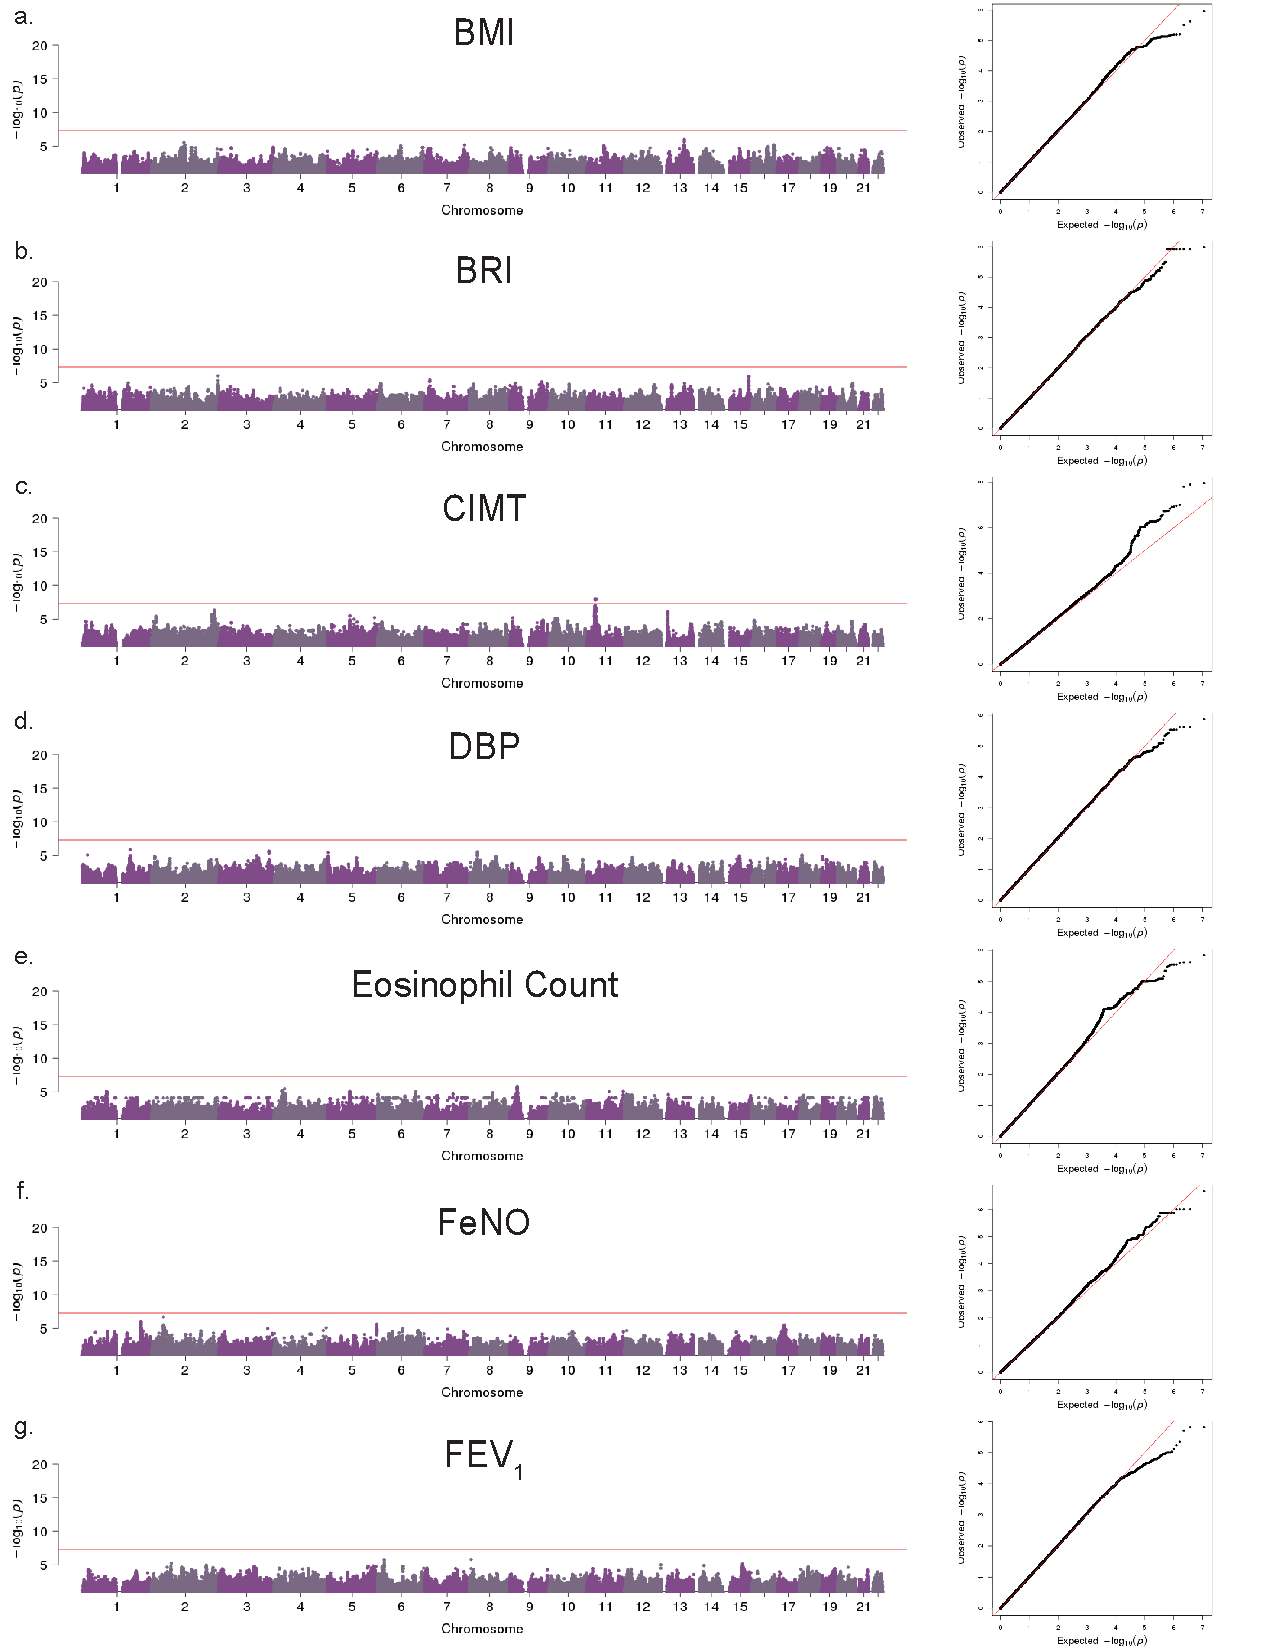
\includegraphics[width=5in]{img/ch02/fig-s1a.pdf}
	\caption[Manhattan and QQ Plots from Standard GWAS of 21 Quantitative Phenotypes.]{\textbf{Manhattan and QQ Plots from Standard GWAS of 21 Quantitative Phenotypes.} }
	\label{fig:fig-s1a}
\end{figure}

\begin{figure}[!htb]
	\ContinuedFloat
	\centering
		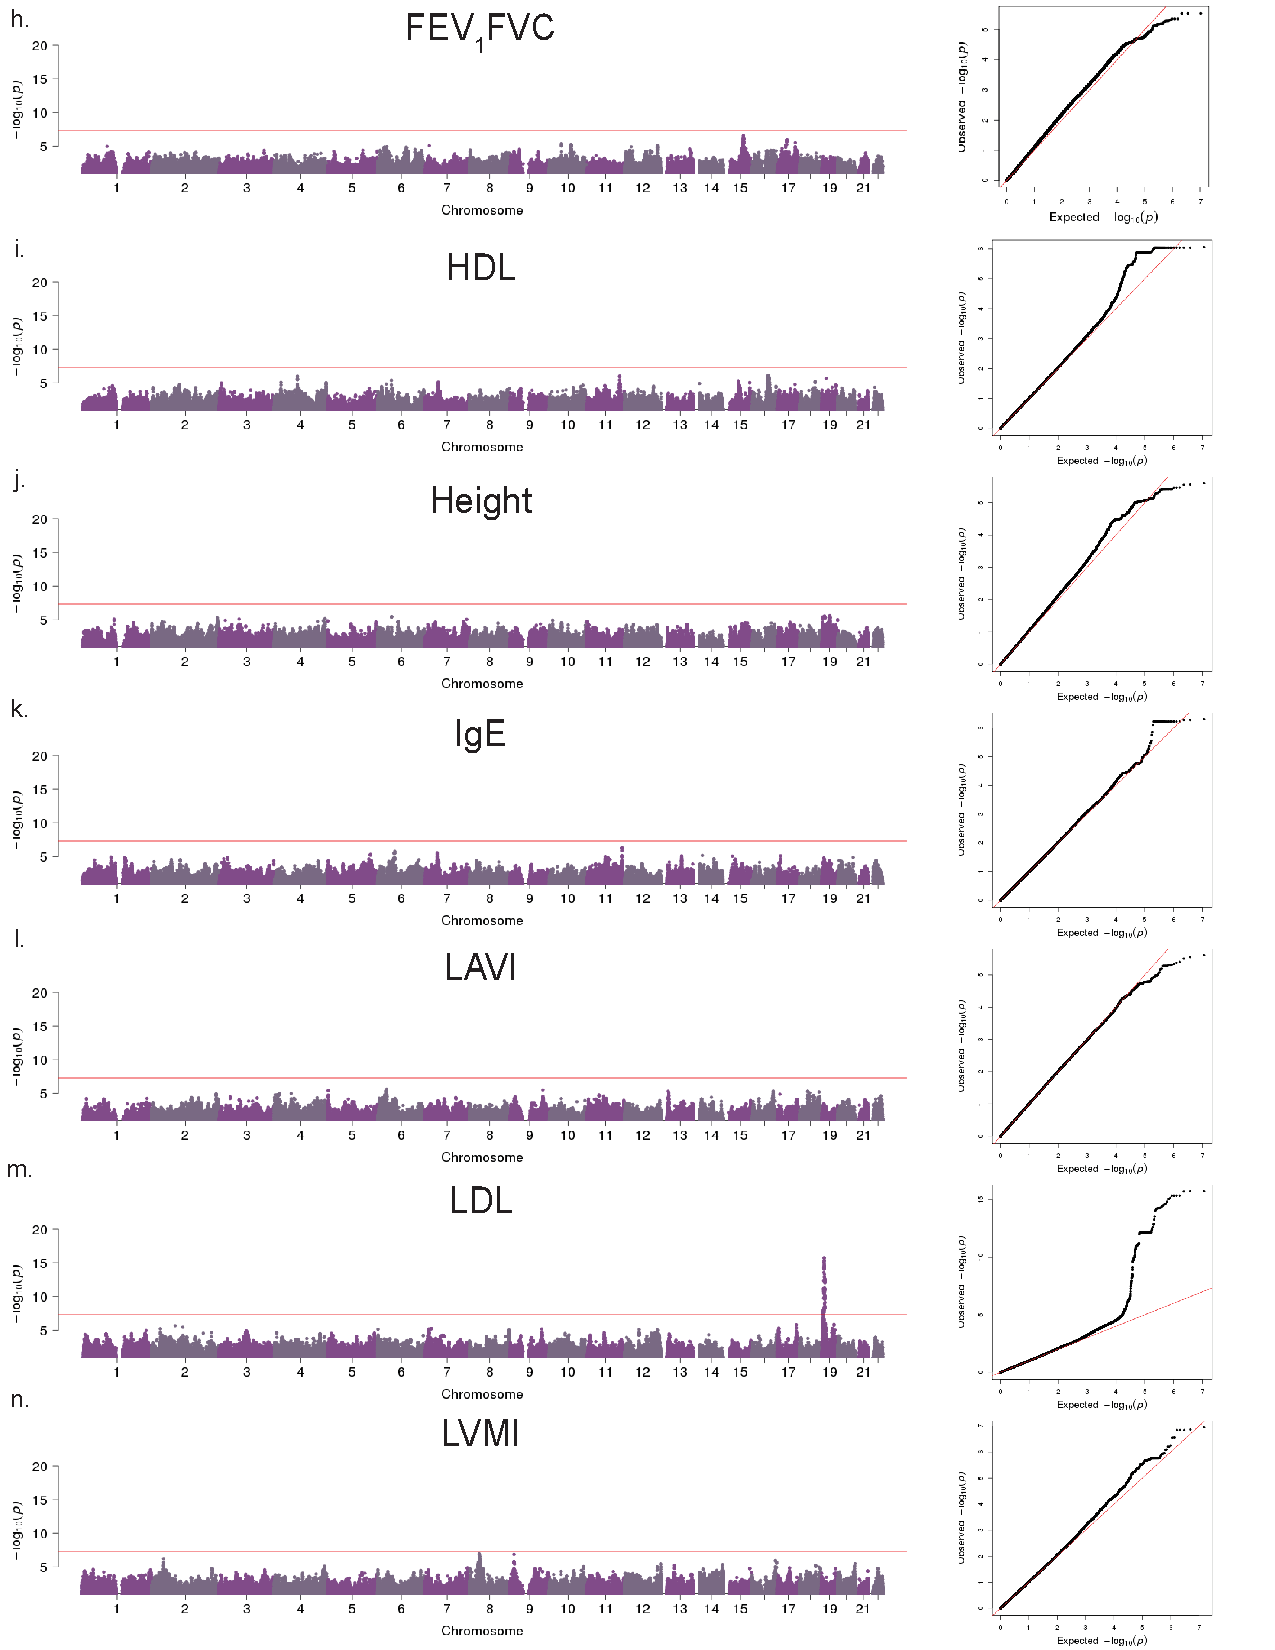
\includegraphics[width=5in]{img/ch02/fig-s1b.pdf}
\caption[Manhattan and QQ Plots from Standard GWAS of 21 Quantitative Phenotypes (Continued).]{\textbf{Manhattan and QQ Plots from Standard GWAS of 21 Quantitative Phenotypes (Continued).} }
\label{fig:fig-s1b}
\end{figure}

 
\begin{figure}[!htb]
\ContinuedFloat
\centering
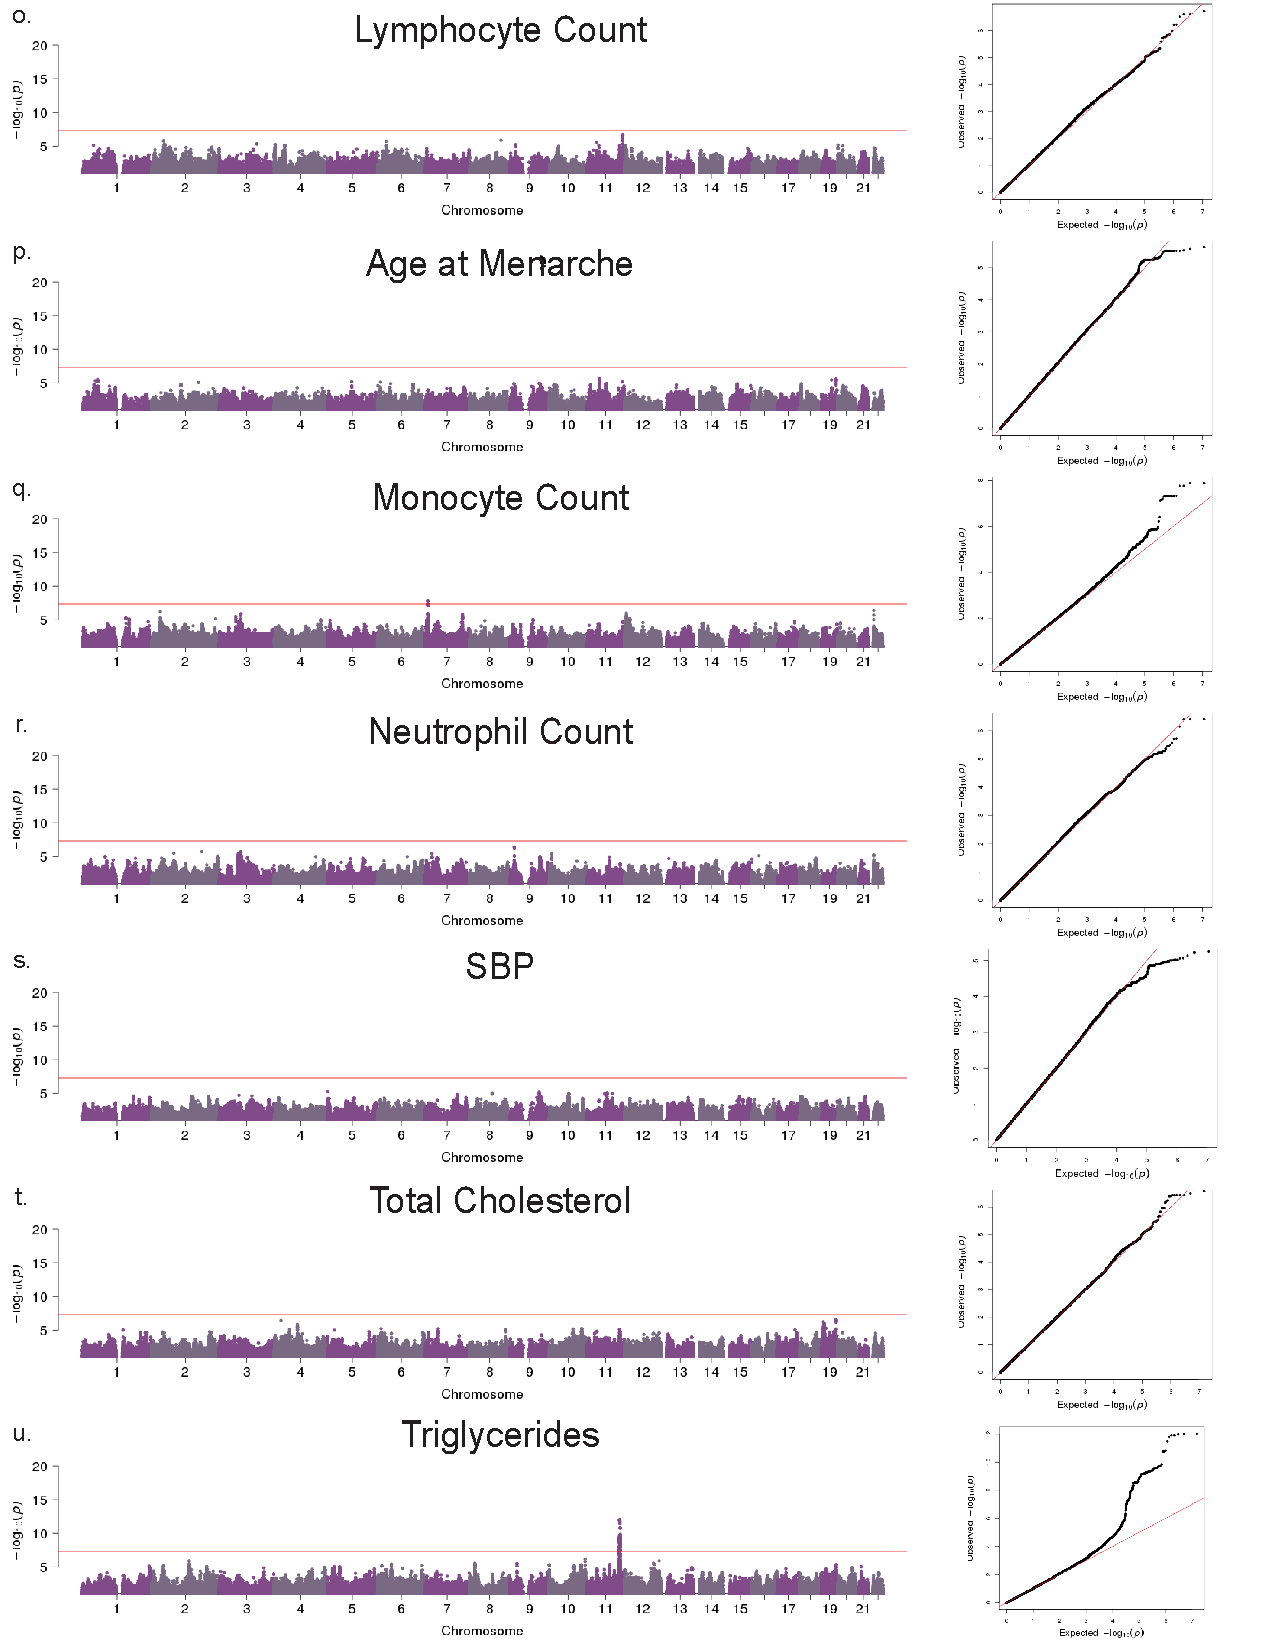
\includegraphics[width=5in]{img/ch02/fig-s1c.pdf}
\caption[Manhattan and QQ Plots from Standard GWAS of 21 Quantitative Phenotypes (Continued).]{\textbf{Manhattan and QQ Plots from Standard GWAS of 21 Quantitative Phenotypes (Continued).} }
\label{fig:fig-s1c}
\end{figure}




\begin{figure}[!htb]
\centering
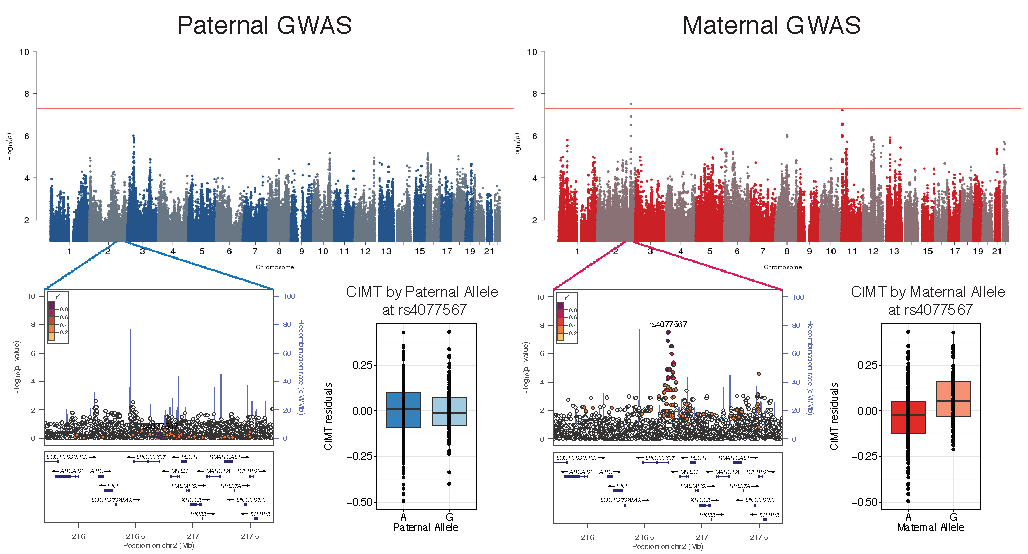
\includegraphics[width=5in]{img/ch02/fig-s2.pdf}
\caption[Maternal and Paternal GWAS results for CIMT.]{\textbf{Maternal and Paternal GWAS results for CIMT.}  The top panel shows the Manhattan plots from the paternal (left) and maternal (right) GWAS. LocusZoom plots are shown in the lower panel for the associated region in the GWAS. Boxplots show the distribution of CIMT residuals (the residuals correspond to the inverse of raw CIMT values) (y-axes) by the corresponding maternal and paternal alleles at this SNP (x-axes). The horizontal bar of the boxplot shows the median, the box delineates the first and third quartile, and the whiskers show +/-1.5 x IQR.}
\label{fig:fig-s2}
\end{figure}



\begin{figure}[!htb]
\centering
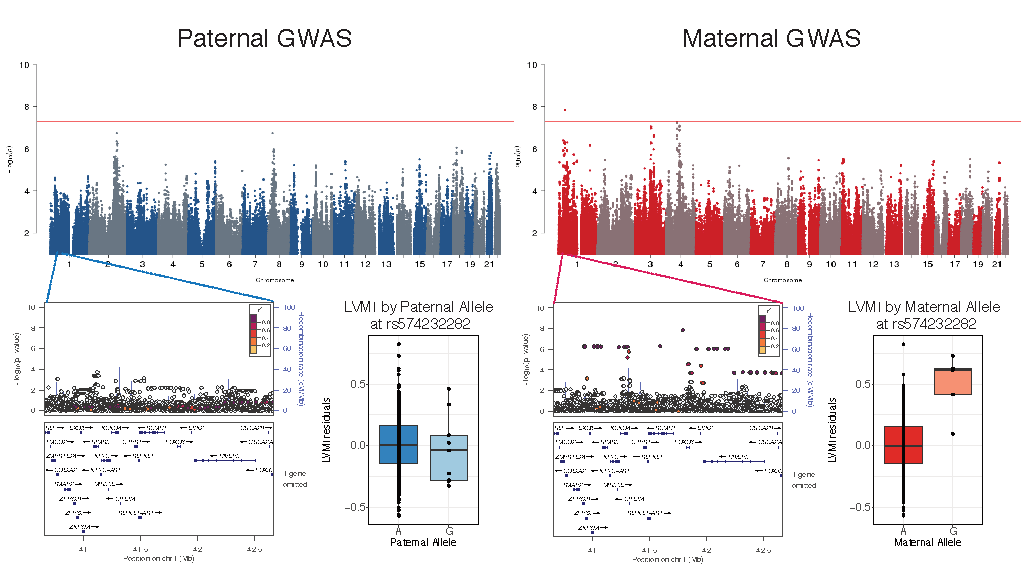
\includegraphics[width=5in]{img/ch02/fig-s3.pdf}
\caption[Maternal and Paternal GWAS results for LVMI.]{\textbf{Maternal and Paternal GWAS results for LVMI.}  The top panel shows the Manhattan plots from the paternal (left) and maternal (right) GWAS. LocusZoom plots are shown in the lower panel for the associated region in the GWAS. Boxplots show the distribution of LVMI residuals (the residuals correspond to the inverse of raw CIMT values) (y-axes) by the corresponding maternal and paternal alleles at this SNP (x-axes). The horizontal bar of the boxplot shows the median, the box delineates the first and third quartile, and the whiskers show +/-1.5 x IQR.}
\label{fig:fig-s3}
\end{figure}



\begin{figure}[!htb]
\centering
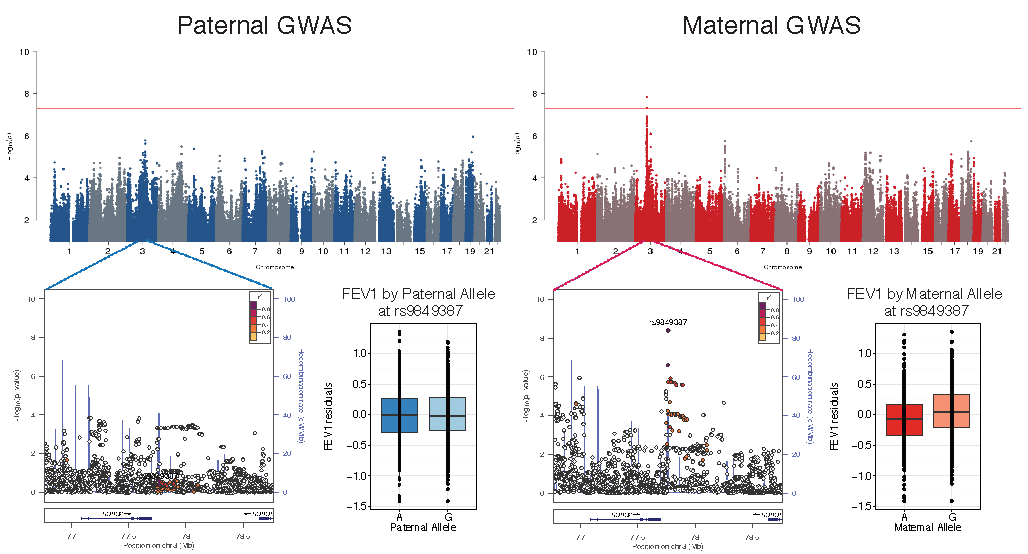
\includegraphics[width=5in]{img/ch02/fig-s4.pdf}
\caption[Maternal and Paternal GWAS results for FEV\textsubscript{1}.]{\textbf{Maternal and Paternal GWAS results for FEV\textsubscript{1}.}  The top panel shows the Manhattan plots from the paternal (left) and maternal (right) GWAS. LocusZoom plots for both GWAS are shown in the lower panel for the associated region in the GWAS. Boxplots show the distribution of FEV\textsubscript{1} residuals (y-axes) by the corresponding maternal and paternal alleles at this SNP (x-axes). The horizontal bar of the boxplot shows the median, the box delineates the first and third quartile, and the whiskers show 1.5 x IQR.}
\label{fig:fig-s4}
\end{figure}




\begin{figure}[!htb]
\centering
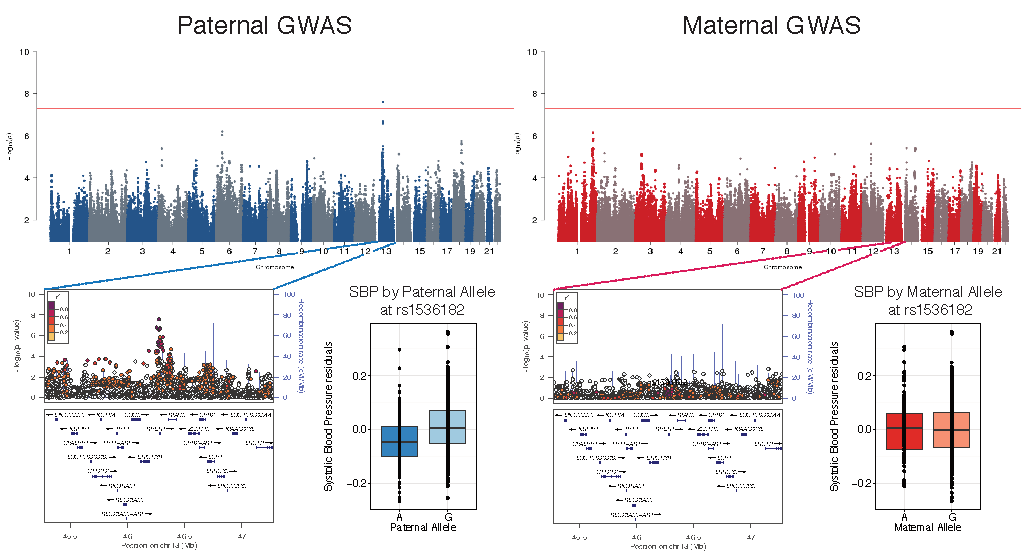
\includegraphics[width=5in]{img/ch02/fig-s5.pdf}
\caption[Maternal and Paternal GWAS results for Systolic Blood Pressure.]{\textbf{Maternal and Paternal GWAS results for Systolic Blood Pressure.}  The top panel shows the Manhattan plots from the paternal (left) and maternal (right) GWAS. LocusZoom plots for both GWAS are shown in the lower panel for the associated region in the GWAS. Boxplots show the distribution of systolic blood pressure residuals (y-axes) by the corresponding maternal and paternal alleles at this SNP (x-axes). The horizontal bar of the boxplot shows the median, the box delineates the first and third quartile, and the whiskers show 1.5 x IQR.}
\label{fig:fig-s5}
\end{figure}




\begin{figure}[!htb]
\centering
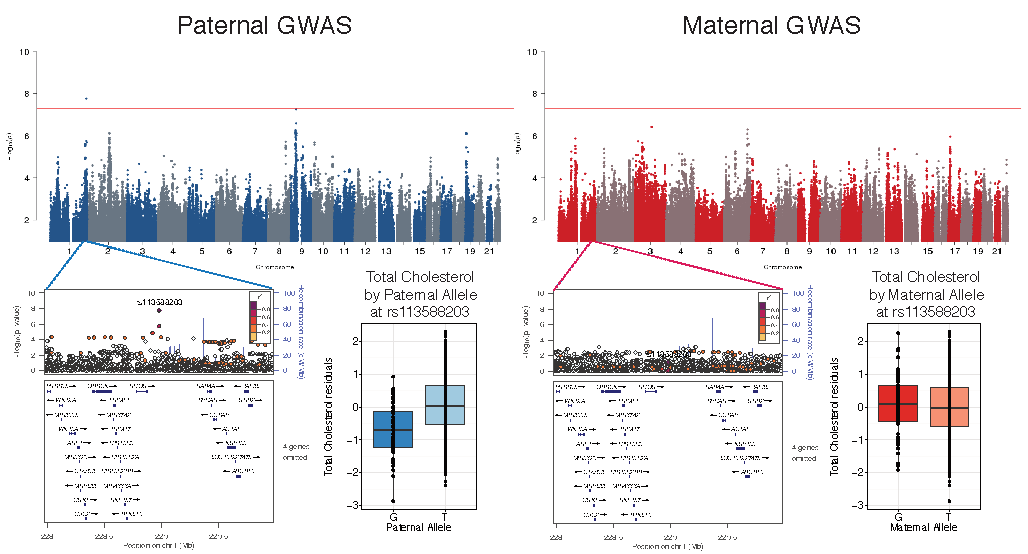
\includegraphics[width=5in]{img/ch02/fig-s6.pdf}
\caption[Maternal and Paternal GWAS results for Total Cholesterol.]{\textbf{Maternal and Paternal GWAS results for Total Cholesterol.}  The top panel shows the Manhattan plots from the paternal (left) and maternal (right) GWAS. LocusZoom plots for both GWAS are shown in the lower panel for the associated region in the GWAS. Boxplots show the distribution of total cholesterol residuals (y-axes) by the corresponding maternal and paternal alleles at this SNP (x-axes). The horizontal bar of the boxplot shows the median, the box delineates the first and third quartile, and the whiskers show 1.5 x IQR.}
\label{fig:fig-s6}
\end{figure}



\begin{figure}[!htb]
	\centering
	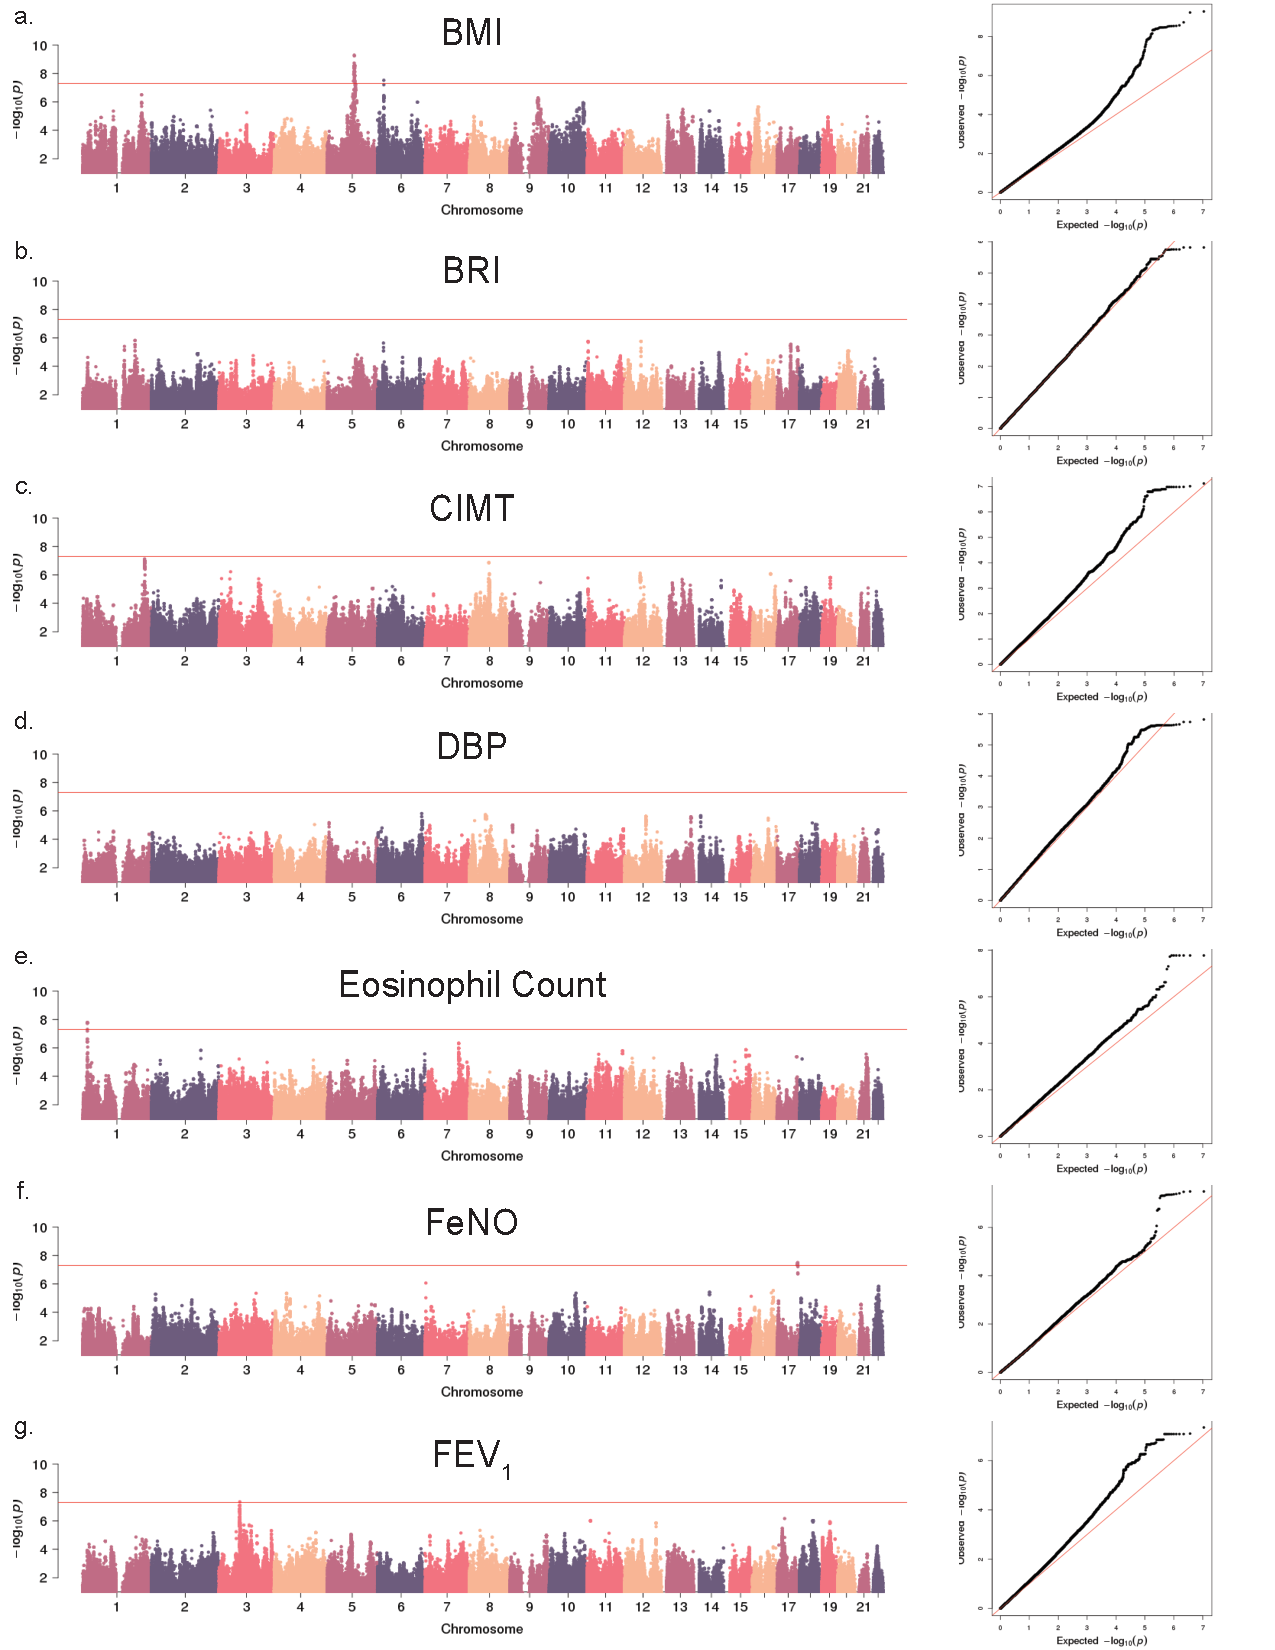
\includegraphics[width=5in]{img/ch02/fig-s7a.pdf}
	\caption[Manhattan and QQ Plots from Differential Effect GWAS of 21 Quantitative Phenotypes. ]{\textbf{Manhattan and QQ Plots from Differential Effect GWAS of 21 Quantitative Phenotypes .} }
	\label{fig:fig-s7a}
\end{figure}


\begin{figure}[!htb]
	\ContinuedFloat
	\centering
	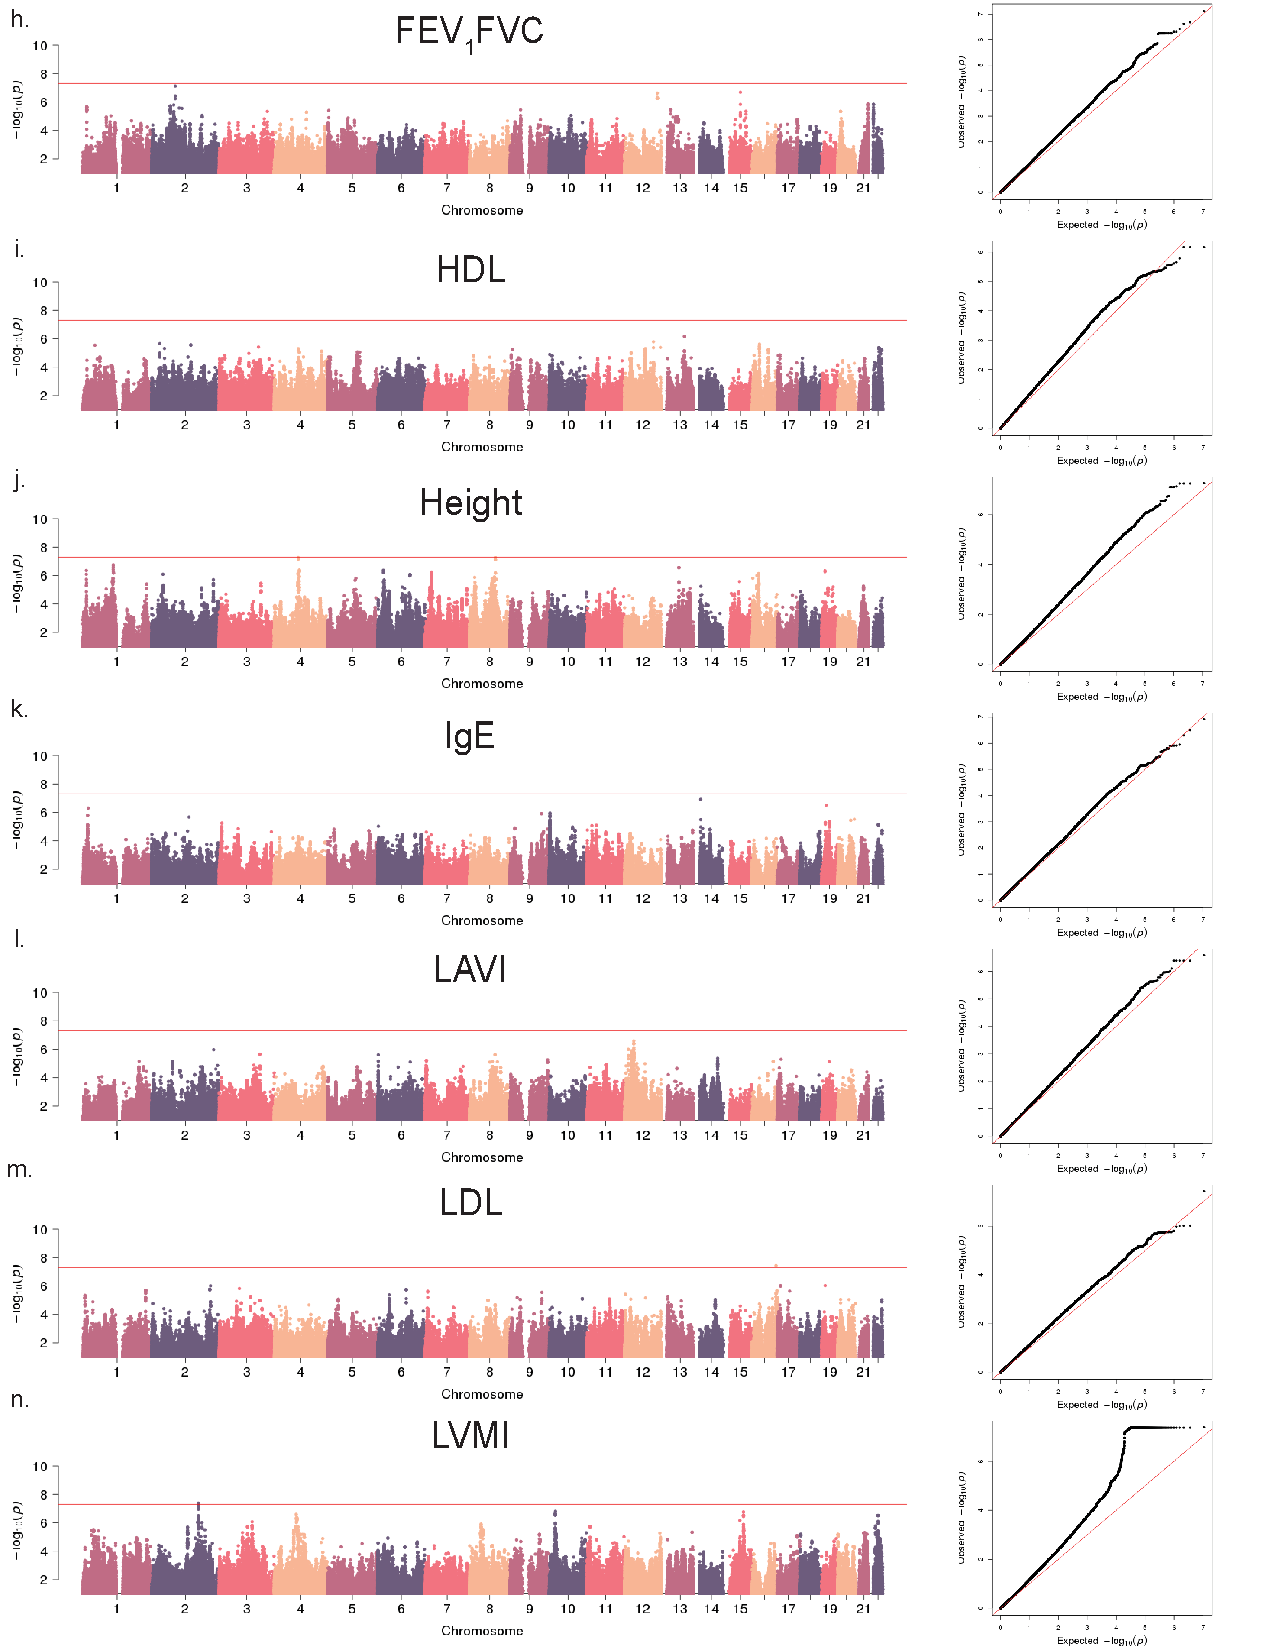
\includegraphics[width=5in]{img/ch02/fig-s7b.pdf}
	\caption[Manhattan and QQ Plots from Differential Effect GWAS of 21 Quantitative Phenotypes (Continued). ]{\textbf{Manhattan and QQ Plots from Differential Effect GWAS of 21 Quantitative Phenotypes (Continued).} }
	\label{fig:fig-s7b}
\end{figure}



\begin{figure}[!htb]
	\ContinuedFloat
	\centering
	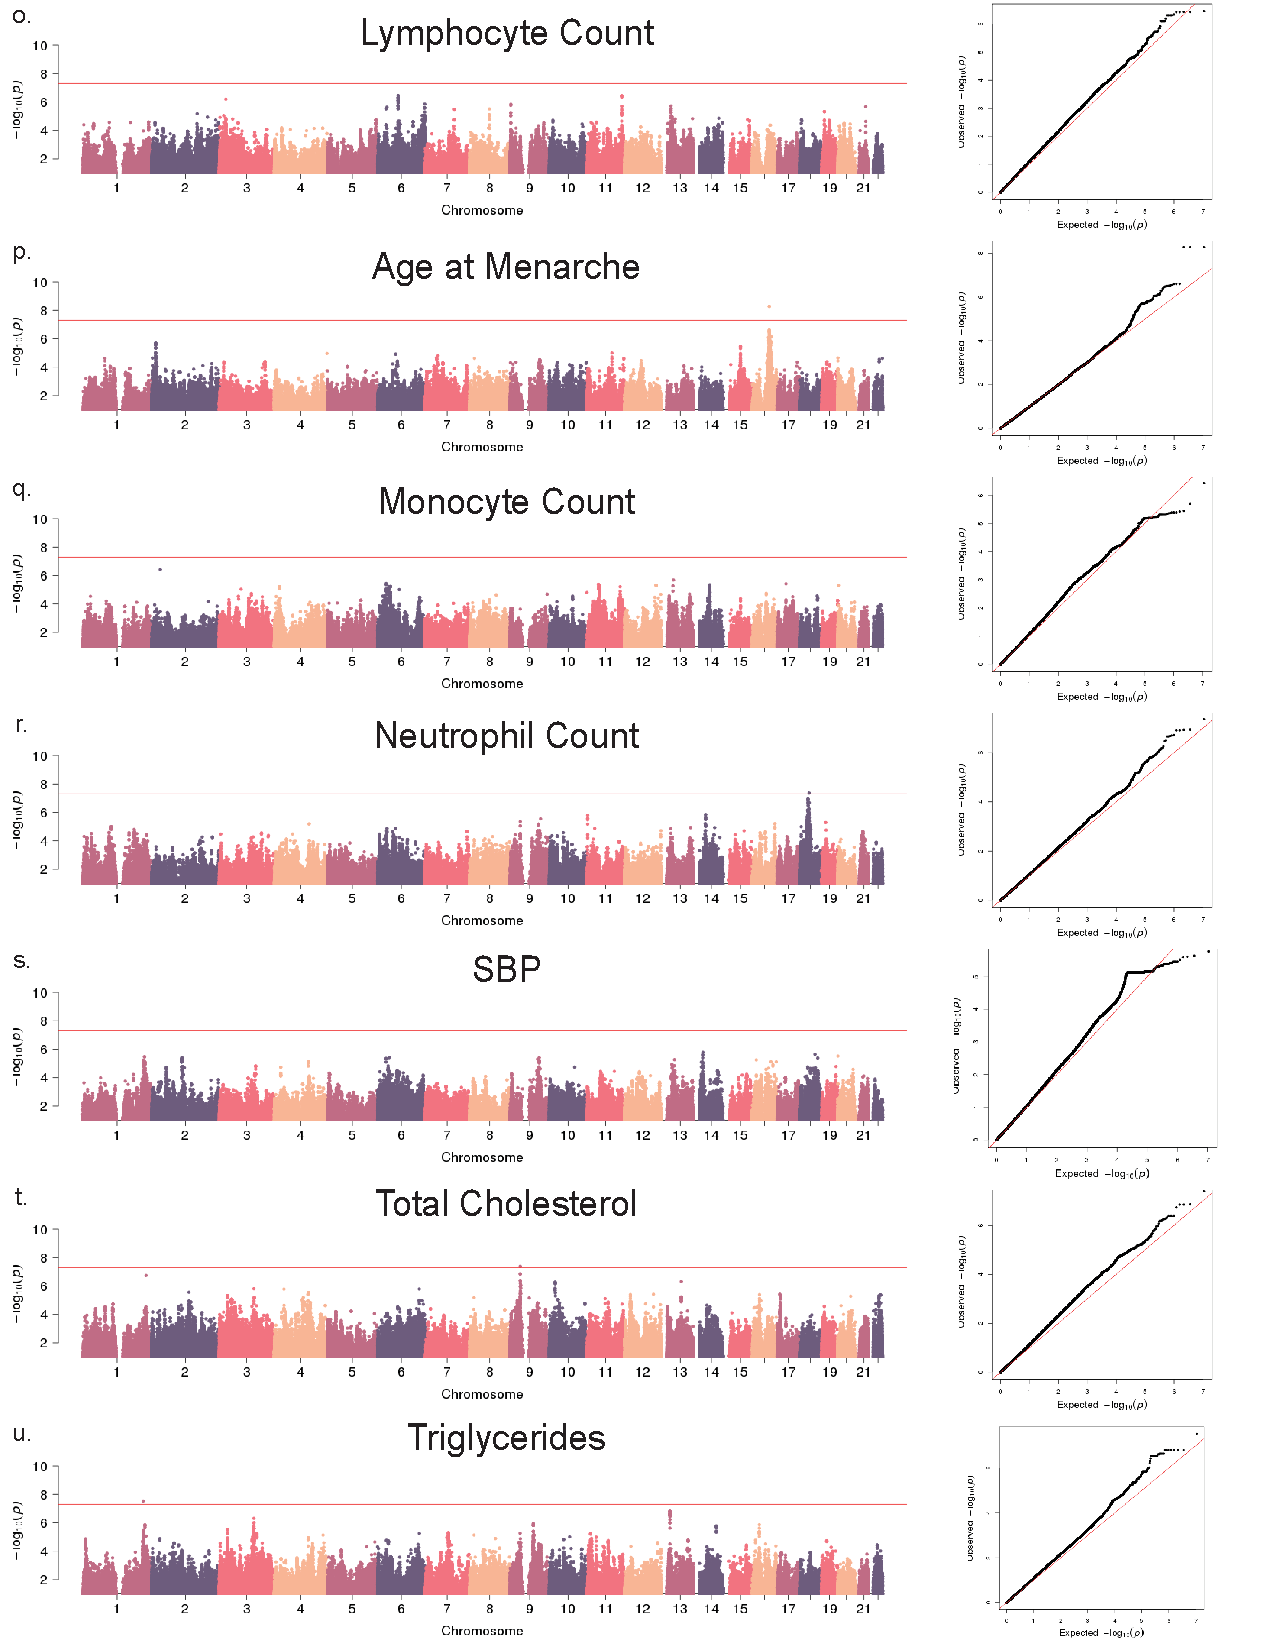
\includegraphics[width=5in]{img/ch02/fig-s7c.pdf}
	\caption[Manhattan and QQ Plots from Differential Effect GWAS of 21 Quantitative Phenotypes (Continued). ]{\textbf{Manhattan and QQ Plots from Differential Effect GWAS of 21 Quantitative Phenotypes (Continued).} }
	\label{fig:fig-s7c}
\end{figure}


\begin{figure}[!htb]
\centering
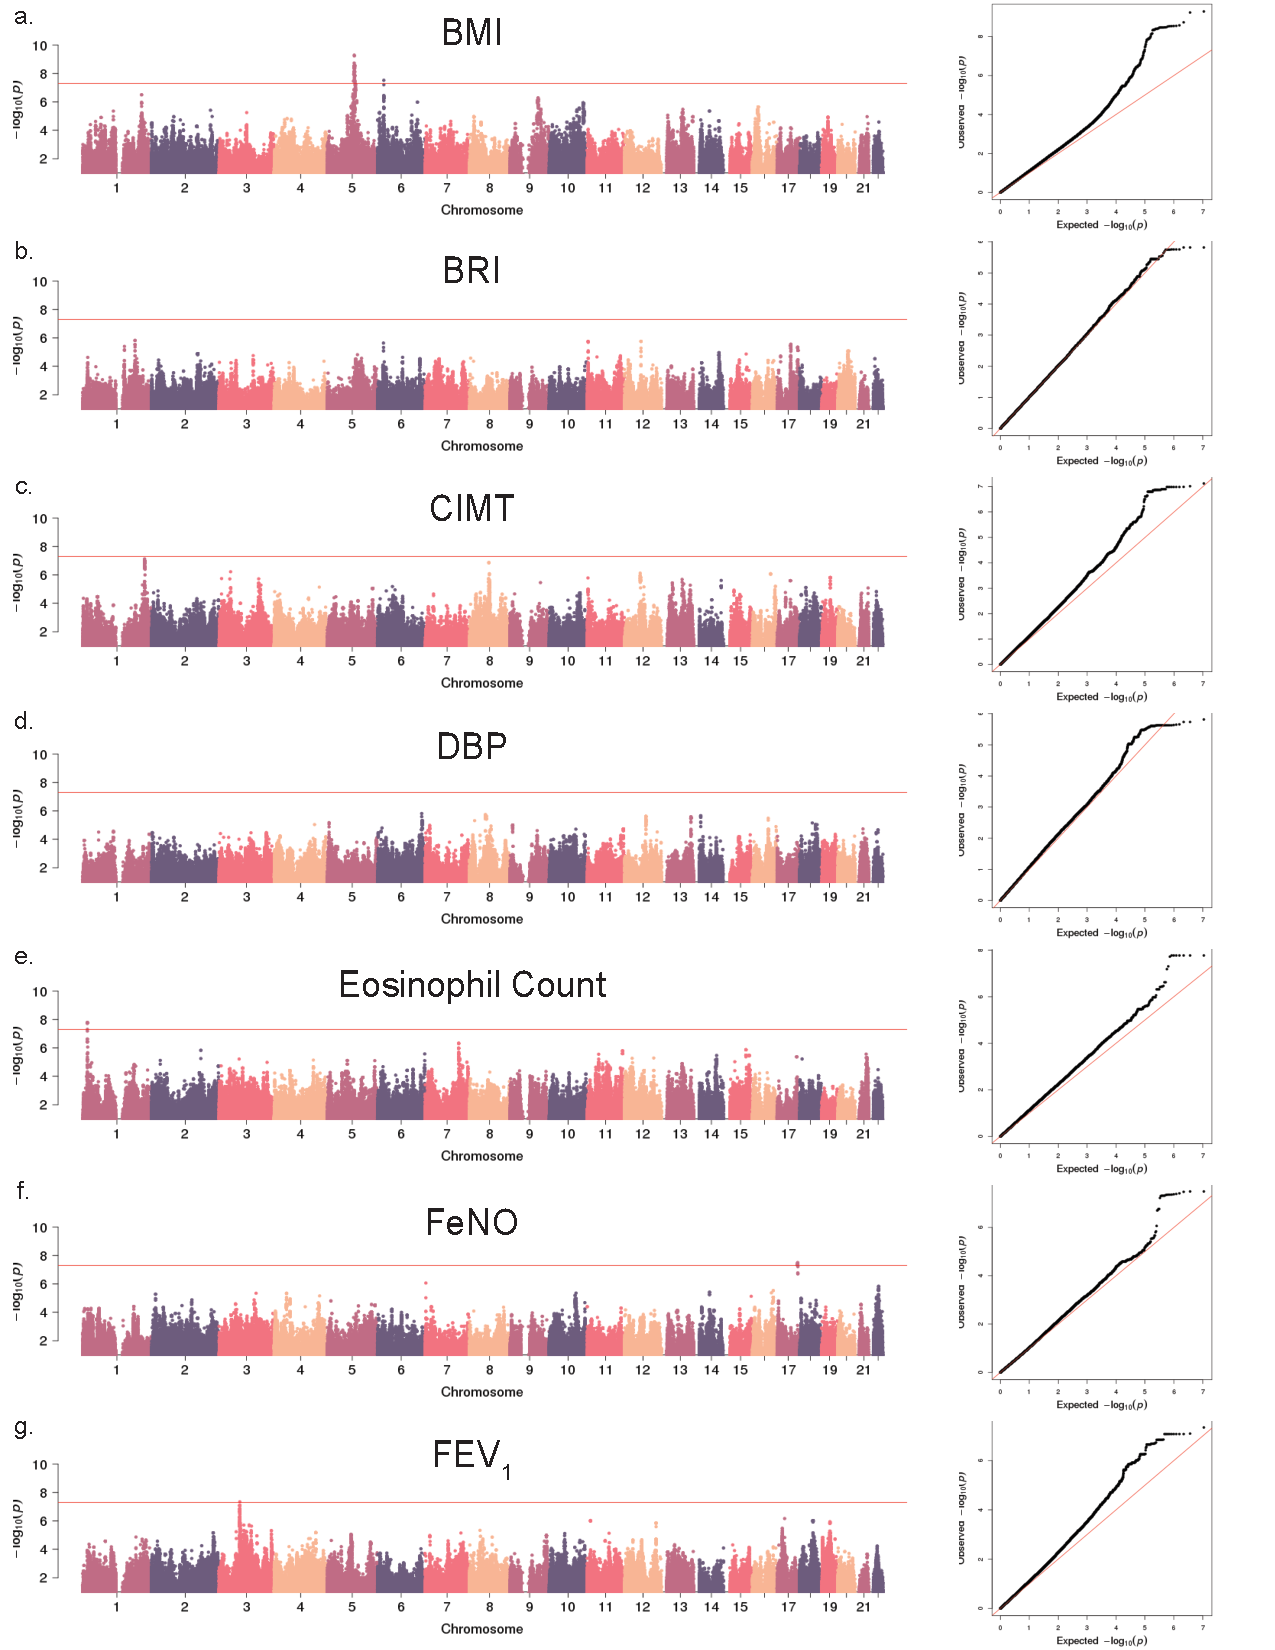
\includegraphics[width=5in]{img/ch02/fig-s8.pdf}
\caption[Opposite Effect Parent-of-Origin GWAS Result for LDL.]{\textbf{Opposite Effect Parent-of-Origin GWAS Result for LDL.}  Box plots of LDL residuals (y-axes) are shown for each of the four genotypes (left panel; x-axis), and for paternal (center panel; x-axis) and maternal (right panel; x-axis) alleles. The maternal G allele is associated with decreased and maternal A allele with increased LDL. The paternal G allele is associated with increased and the paternal A allele with decreased LDL. The horizontal bar of the boxplot shows the median, the box delineates the first and third quartile, and the whiskers show +/-1.5 x IQR.}
\label{fig:fig-s8}
\end{figure}

\begin{figure}[!htb]
\centering
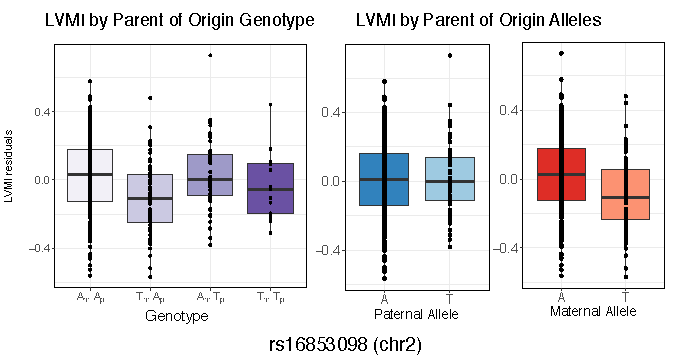
\includegraphics[width=5in]{img/ch02/fig-s9.pdf}
\caption[Opposite Effect Parent-of-Origin GWAS Result for LVMI.]{\textbf{Opposite Effect Parent-of-Origin GWAS Result for LVMI.}  Box plots of LVMI residuals (y-axes) are shown for each of the four genotypes (left panel; x-axis), and for paternal (center panel; x-axis) and maternal (right panel; x-axis) alleles. The maternal T allele is associated with decreased and maternal A allele with increased LVMI. The paternal T allele is associated with increased and the paternal A allele with decreased LVMI. The horizontal bar of the boxplot shows the median, the box delineates the first and third quartile, and the whiskers show +/-1.5 x IQR.}
\label{fig:fig-s9}
\end{figure}

\begin{figure}[!htb]
\centering
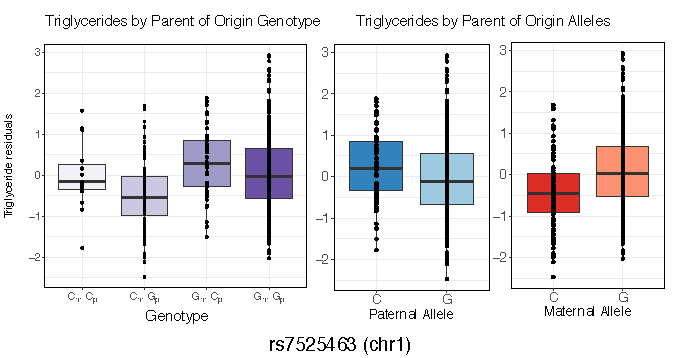
\includegraphics[width=5in]{img/ch02/fig-s10.pdf}
\caption[Opposite Effect Parent-of-Origin GWAS Result for Triglycerides.]{\textbf{Opposite Effect Parent-of-Origin GWAS Result for Triglycerides.}  Box plots of triglyceride residuals (y-axes) are shown for each of the four genotypes (left panel; x-axis), and for paternal (center panel; x-axis) and maternal (right panel; x-axis) alleles. The maternal C allele is associated with decreased and maternal G allele with increased triglycerides. The paternal C allele is associated with increased and the paternal G allele with decreased triglycerides. The horizontal bar of the boxplot shows the median, the box delineates the first and third quartile, and the whiskers show +/-1.5 x IQR.}
\label{fig:fig-s10}
\end{figure}

\begin{figure}[!htb]
\centering
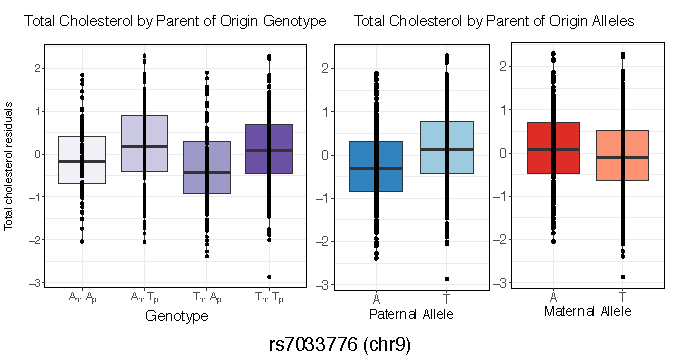
\includegraphics[width=5in]{img/ch02/fig-s11.pdf}
\caption[Opposite Effect Parent-of-Origin GWAS Result for Total Cholesterol.]{\textbf{Opposite Effect Parent-of-Origin GWAS Result for Total Cholesterol.}  Box plots of total cholesterol residuals (y-axes) are shown for each of the four genotypes (left panel; x-axis), and for paternal (center panel; x-axis) and maternal (right panel; x-axis) alleles. The maternal T allele is associated with decreased and maternal A allele with increased total cholesterol. The paternal T allele is associated with increased and the paternal A allele with decreased total cholesterol. The horizontal bar of the boxplot shows the median, the box delineates the first and third quartile, and the whiskers show +/-1.5 x IQR.}
\label{fig:fig-s11}
\end{figure}

\begin{figure}[!htb]
\centering
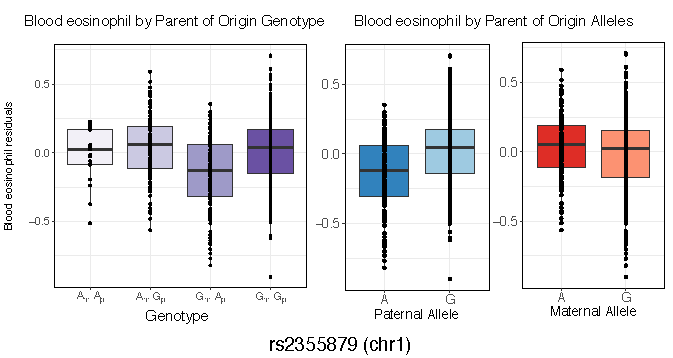
\includegraphics[width=5in]{img/ch02/fig-s12.pdf}
\caption[Opposite Effect Parent-of-Origin GWAS Result for Blood Eosinophil Count.]{\textbf{Opposite Effect Parent-of-Origin GWAS Result for Blood Eosinophil Count.}  Box plots of eosinophil residuals (y-axes) are shown for each of the four genotypes (left panel; x-axis), and for paternal (center panel; x-axis) and maternal (right panel; x-axis) alleles. The maternal G allele is associated with decreased and maternal A allele with increased eosinophil count. The paternal G allele is associated with increased and the paternal A allele with decreased eosinophil count. The horizontal bar of the boxplot shows the median, the box delineates the first and third quartile, and the whiskers show +/-1.5 x IQR.}
\label{fig:fig-s12}
\end{figure}

\begin{figure}[!htb]
\centering
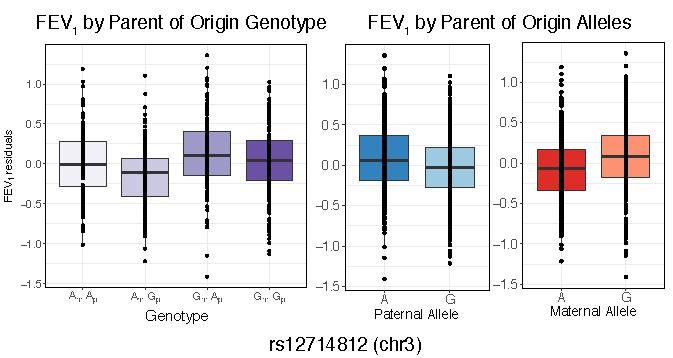
\includegraphics[width=5in]{img/ch02/fig-s13.pdf}
\caption[Opposite Effect Parent-of-Origin GWAS Result for FEV\textsubscript{1}.]{\textbf{Opposite Effect Parent-of-Origin GWAS Result for FEV\textsubscript{1}.} Box plots of FEV\textsubscript{1} residuals (y-axes) are shown for each of the four genotypes (left panel; x-axis), and for paternal (center panel; x-axis) and maternal (right panel; x-axis) alleles. The maternal A allele is associated with decreased and maternal G allele with increased FEV\textsubscript{1}. The paternal A allele is associated with increased and the paternal G allele with decreased FEV\textsubscript{1}. The horizontal bar of the boxplot shows the median, the box delineates the first and third quartile, and the whiskers show +/-1.5 x IQR.}
\label{fig:fig-s13}
\end{figure}

\begin{figure}[!htb]
\centering
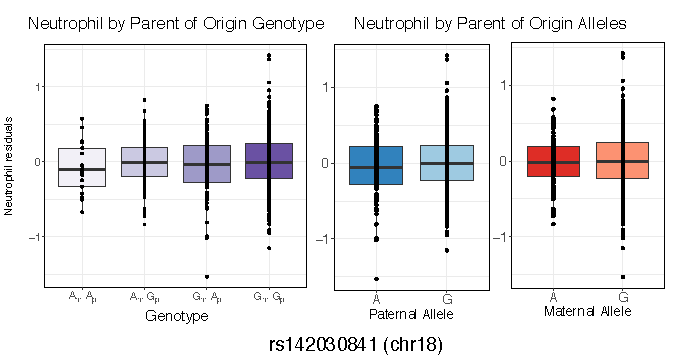
\includegraphics[width=5in]{img/ch02/fig-s14.pdf}
\caption[Opposite Effect Parent-of-Origin GWAS Result for Neutrophil Count.]{\textbf{Opposite Effect Parent-of-Origin GWAS Result for Neutrophil Count.}  Box plots of neutrophil residuals (y-axes) are shown for each of the four genotypes (left panel; x-axis), and for paternal (center panel; x-axis) and maternal (right panel; x-axis) alleles. The maternal G allele is associated with decreased and maternal A allele with increased neutrophil count. The paternal G allele is associated with increased and the paternal A allele with decreased neutrophil count. The horizontal bar of the boxplot shows the median, the box delineates the first and third quartile, and the whiskers show +/-1.5 x IQR.}
\label{fig:fig-s14}
\end{figure}






\begin{figure}[!htb]
\centering
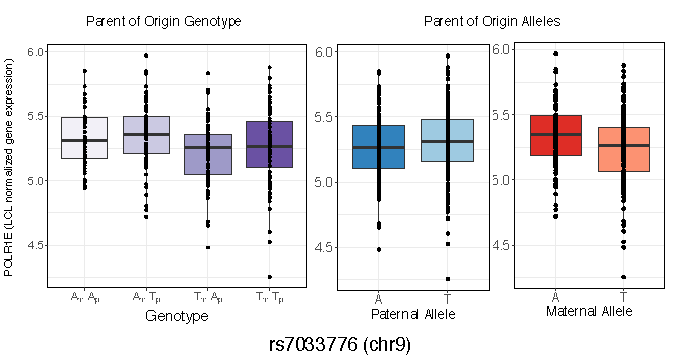
\includegraphics[width=5in]{img/ch02/fig-s15.pdf}
\caption[Opposite Effect eQTL for rs7033776.]{\textbf{Opposite Effect eQTL for rs7033776.} Box plots of two significant loci plot \emph{POLR1E} gene expression residuals (y-axes) for each of the four genotypes (left panel; x-axis), and for paternal (center panel; x-axis) and maternal (right panel; x-axis) alleles. The maternal T allele is associated with decreased and maternal A allele with increased \emph{POLR1E} expression. The paternal T allele is associated with increased and the paternal A allele with decreased \emph{POLR1E} expression. The horizontal bar of the boxplot shows the median, the box delineates the first and third quartile, and the whiskers show +/-1.5 x IQR.}
\label{fig:fig-s15}
\end{figure}



\begin{landscape}

\begin{table}
\centering
\begin{adjustbox}{width={\textwidth}}
\begin{tabular}{@{}p{2.5cm}|p{1cm}p{2cm}p{2cm}p{1cm}p{1cm}p{4cm}p{3cm}|p{5cm}@{}}
\toprule Quantitative Trait & Sample Size & M/F Ratio & Age range (years) & GWAS call rate & PO call rate & Transformation & Covariates & Exclusions\\ \midrule
SBP & 807 & 	371/436 & 	6-85 & 	0.94 & 	0.82 & 	log & 	age, sex, age*sex, technician & \multirow{2}{5cm}{Anti-hypertensive medication} \\ \cline{1-8}
DBP & 807 & 	371/436 & 	6-85 & 	0.94 & 	0.82 & 	log & 	age, sex, age*sex, inbreeding, technician	 & \\ \hline
HDL & 828 & 	381/447 & 	14-85 & 	0.94 & 	0.80 & 	cube root & 	age, sex	& \multirow{4}{5cm}{Anti-hypercholesterolemia medication, hormone replacement therapy, birth control; diagnosis of sitosterolemia} \\ \cline{1-8}
LDL & 807 & 	367/440 & 	14-85 & 	- &	0.80 & 	cube root	age, sex	& \\ \cline{1-8}
Triglycerides & 828 & 382/446	14-85 & 	0.94	&0.80	&log	&age, sex	& \\ \cline{1-8}
Total cholesterol/HDL&	828 & 381/447&	14-85&	0.94&	0.80	&log	&age, sex	& \\ \hline
Monocyte count & 1069&	503/566&	5.47-85.10	&0.94&	0.81&	log&	age, sex, age*sex & \multirow{4}{5cm}{Antibiotics, immunosupressants, and/or steroids was an exclusion for all WBC count phenotypes. Antifungal medication was an exclusion for the Eosinophil Count phenotype.}\\ \cline{1-8}
Lymphocyte count & 1079 & 	507/572	&6-85 & 	0.94	 & - &	log	 & age	 & \\ \cline{1-8}
Eosinophil count & 1068 & 	502/566 & 	5.47-85.10	 & 0.94	 & 0.81	 & square root(log()) & 	sex	 & \\ \cline{1-8}
Neutrophil count & 1070 & 	503/567 & 	5.47-85.10 & 	0.94	 & 0.81	 & log	 & age, sex, age*sex, phase	 & \\ \cline{1-8}
LAVI & 637 & 	296/341 & 	14-88 & 	0.94 & 	0.80	 & log & 	age, sex & 	Pregnant, history of heart valve replacement, or poor quality echocardiography images \\ \hline
LVMI	 & 621 & 	286/335 & 	14-88 & 	0.94	 & 0.79 & 	log	 & age, sex	 & Aortic stenosis by history or echocardiogram Cholesterol and/or thyroid medication or poor quality echocardiography images \\ \hline
CIMT & 547 & 248/299 & 	14-86 & 	0.94 & 	0.80 & 	inverse & 	age, sex	 & Cholesterol and/or thyroid medication, history of liver disease, or poor quality imaging \\ \hline
FeNO & 825 & 381/444 & 	6-85 & 	0.95 & 	0.82 & 	log & 	age, sex, technician	 & Poor quality measurements  \\ \bottomrule
\end{tabular}
\end{adjustbox}
\caption[Summary of the Hutterite Phenotypes and Sample Composition. ]{\textbf{Summary of the Hutterite Phenotypes and Sample Composition.} *SBP: Systolic Blood Pressure, DBP: Diastolic Blood Pressure, HDL: High Density Lipoprotein, LDL: Low Density Lipoprotein, LAVI: Left Atrial Volume Index, LVMI: Left Ventricular Mass Index, CIMT: Carotid Intima Media Thickness, FeNO: Fraction of Exhaled Nitric Oxide, FEV\textsubscript{1}: Forced Expiratory Volume at 1 s, FVC: Forced Vital Capacity, BRI: Bronchial Responsiveness Index}
\label{tab:tab-s1a}
\end{table}


\begin{table}
\centering
\begin{adjustbox}{width={\textwidth}}
\begin{tabular}{@{}p{2.5cm}|p{1cm}p{2cm}p{2cm}p{1cm}p{1cm}p{4cm}p{3cm}|p{5cm}@{}}
\toprule Quantitative Trait & Sample Size & M/F Ratio & Age range (years) & GWAS call rate & PO call rate & Transformation & Covariates & Exclusions\\ \midrule
BRI & 950	 & 445/505 & 	6.11-78.22 & 	0.94	 & 0.82	 & none	 & age, inbreeding & 	Pregnant and/or lactating or medical contraindications (e.g. beta-blockers, asthma medication 24 hour prior to examination, cystic fibrosis) \\ \hline
FEV\textsubscript{1} & 1102 & 509/593 & 	5.47-8.47	 & 0.94 &	0.82 & 	none	 & Age, sex, height, height squared, phase, sex * age group (<17 vs $\geq$ 17 years old), age*sex*age group, height*sex*age group	 & \multirow{2}{5cm}{Poor quality FEV1 and/or FVC measurements or medical contraindications (e.g. asthma medication 24 hour prior to examination, cystic fibrosis)} \\ \cline{1-8}
FEV\textsubscript{1}/FVC & 1106 & 512/594 & 	5.47-8.47 & 	0.94	 & 0.82 & 	none & 	age, sex, age*sex, inbreeding	 & \\ \hline
Total serum IgE	 & 1219 & 562/657 & 	6-91	 & 0.94 & 	0.81 & 	log	 & age	 & Xolair medication \\ \hline
BMI & 1188 & 	577/652 & 5.5-89.2 & 	0.94	 & 0.82 & 	log & 	log(age), sex, phase, colony	 & Pregnancy \\ \hline
Height & 1199 & 576/669 & 5-89 & 	0.94 & 	0.82 & 	none	& age, age*sex group (<15 years old males+females), age*sex ($\geq$ 15 years old males), age*sex  $\geq$ 15 years old females)	 & - \\ \hline
Age at menarche & 477 & 0/719 & 	9-17 & 	0.92 & 	0.71	 & none & 	birthyear	 & - \\ \bottomrule
\end{tabular}
\end{adjustbox}
\caption[Summary of the Hutterite Phenotypes and Sample Composition (Continued). ]{\textbf{Summary of the Hutterite Phenotypes and Sample Composition (Continued).} *SBP: Systolic Blood Pressure, DBP: Diastolic Blood Pressure, HDL: High Density Lipoprotein, LDL: Low Density Lipoprotein, LAVI: Left Atrial Volume Index, LVMI: Left Ventricular Mass Index, CIMT: Carotid Intima Media Thickness, FeNO: Fraction of Exhaled Nitric Oxide, FEV\textsubscript{1}: Forced Expiratory Volume at 1 s, FVC: Forced Vital Capacity, BRI: Bronchial Responsiveness Index}
\label{tab:tab-s1b}
\end{table}



\end{landscape}


\begin{landscape}

\begin{table}
\centering
\begin{adjustbox}{width={\textwidth}}
\begin{tabular}{@{}p{2cm}|p{2.5cm}p{4cm}p{3cm}p{2cm}p{3cm}p{2.1cm}p{1.5cm}p{3cm}p{2cm}@{}}
\toprule Phenotype & Sample size & Most significant GWAS p-value & SNP Sample Size & rsid (Effect allele/Other allele) & chr:loc & Beta (SE) & Variant & (Nearest) Gene & MAF \\ \midrule

BMI & 1188 & 8.04E-07 & 1016	 & rs139659764 (A/G) & 13:81274241 & -8.16E-02 (1.64E-02) & intergenic & \emph{LINC00377} & 0.07555 \\ \hline

BRI & 950 & 3.05E-07 & 935 & rs7498042 (T/G) & 15:91119014 & 3.34E-02        (6.47E-03) & intron & \emph{CRTC3} & 0.2921\\ \hline

CIMT & 547 & 1.51E-09 & 470 & rs116908536 (A/G) & 11:33699981 & -0.144         (2.34E-02) & intron & \emph{LOC105376617} & 0.05183\\ \hline

DBP & 807 & 9.66E-07 & 999 & rs116196949 (T/C) & 18:9014768 & -4.84E-02         (9.82E-03) & intergenic & \emph{NDUFV2} & 0.1312\\ \hline

Eosinophil count & 1068 & 1.44E-07 & 939 & rs62544465 (A/G) & 9:26045558 & 8.17E-02     (1.68E-02) & intergenic & \emph{LOC100506422} & 0.147\\ \hline

FeNO & 825 & 2.15E-07 & 753 & rs1121780 (T/C) & 2:42961321 & 0.157      (2.96E-02) & intron & \emph{MTA3} & 0.4824\\ \hline

FEV\textsubscript{1} & 1102 & 1.22E-06 & 1102 & rs13281444 (C/T) & 8:6520628 & 1.11E-01       (2.28E-02) & intron & \emph{LOC100507530} & 0.358\\ \hline

FEV\textsubscript{1}/FVC & 1106 & 2.49E-07 & 1099 & rs8028898 (A/G) & 15:71679543	 & -2.75E-01       (5.31E-02) & intron & \emph{THSD4} & 0.2049\\ \hline

HDL & 828 & 8.81E-07 & 828 & rs186133312 (A/T) & 16:58850424 & -0.483        (9.73E-02) & intergenic	 & \emph{GOT2} & 0.0687\\ \hline

Height & 1199 & 7.62E-07	 & 1009 & rs1318252 (G/A) & 11:1653200 & 1.38         (0.278) & intergenic & \emph{KRTAP5-5} & 0.4239\\ \hline

IgE & 1219 & 3.99E-07 & 1187 & rs66498879 (C/T) & 11:125495211 & -0.256        (5.045E-02) & 5\rq UTR & \emph{CHEK1} & 0.3243\\ \hline

LAVI & 637 & 3.07E-06 & 573 & rs17205373 (G/C) & 6:32626210 & -0.1144        (2.81E-02) & intergenic & \emph{HLA-DQB1} & 0.09724\\ \hline

LDL & 807 & 2.83E-17 & 714 & rs557778817 (T/C) & 19:11305534 & 1.3         (0.15) & intron & \emph{KANK2} & 0.03382\\ \hline

LVMI	 & 621 & 1.23E-09 & 517 & rs113389683 (A/G) & 8:36026788 & 0.153      (2.47E-02) & intergenic & \emph{UNC5D, KCNU1} & 0.08624\\ \hline

Lymphocyte count & 1079 & 5.67E-08 & 894 & rs4323874 (G/A) & 11:129110347 & 8.19E-02 (1.49E-02) & intergenic & \emph{ARHGAP32} & 0.4395\\ \hline
Age at Menarche & 477 & 3.17E-07 & 463 & rs785474 (G/C) & 1:46609106 & 4.5E-01 (8.72E-02) & intron & \emph{PIK3R3} & 0.4268\\ \hline
Monocyte count & 1069 & 1.36E-08 & 902 & rs531317434 (G/T) & 7:9466593 & -0.27 (4.73E-02) & intergenic & \emph{NXPH1, PER4} & 0.03361\\ \hline
Neutrophil count & 1070 & 2.1E-07 & 1070 & rs1215134 (C/T) & 9:15347518 & -8.97E-02 (1.71E-02) & intergenic & \emph{TTC39B} & 0.4307\\ \hline

SBP & 807 & 5.23E-06 & 774 & rs28742608 (G/T) & 5:1440934 & -4.8E-02 (1.05E-02) & intron & \emph{LC6A3} & 0.07549\\ \hline

Total Cholesterol & 828 & 1.20E-07 & 828 & rs11084211 (A/G) & 19:53460861 & 0.287 (5.39E-02) & intron & \emph{ZNF816, ZNF816-ZNF321P} & 0.3071\\ \hline

Triglycerides & 828 & 7.12E-13	 & 707 & rs184333869 (T/C) & 11:117947268 & -1.28 (0.175) & intron & \emph{TMPRSS4} & 0.02399\\ \bottomrule

\end{tabular}
\end{adjustbox}
\caption[GWAS Results. ]{\textbf{GWAS Results.} Phenotype definitions, exclusions, transformations and covariates are summarized in Table \ref{tab:tab-s1a}}
\label{tab:tab-s2}
\end{table}

\end{landscape}




\begin{table}
\centering
\begin{adjustbox}{width={\textwidth}}
\begin{tabular}{@{}p{5cm}|p{5cm}|p{10cm}@{}}
\toprule Phenotype & SNP & genes +/- 1Mb expressed in LCLs\\ \midrule

 \multicolumn{2}{c}{A. Maternal Associations} &\\ \hline
 
 Age at Menarche & rs7184983 & \emph{AMFR, ARL2BP, BBS2, CCDC102A, CCL17, CCL22, CES5A, CETP, CIAPIN1, COQ9, CPNE2, CX2CL1, DOK4, FAM192A, GNAO1, HERPUD1, MR1E, MT1L, MT2A, NLRC5, NUDT21, NUP93, OGFOD1, PLLP, POLR2C, RSPRY1, SLC12A3} \\ \hline
CIMT & rs4077567 & \emph{ABCA12, ATIC, FN1, IGFBP2, MREG, PECR, RPL37A, SMARCAL1, TMEM169, XRCC5} \\ \hline

\multirow{2}{5cm}{FEV1} & rs9849387 & \emph{ROBO1} \\ \cline{2-3}
 & rs6791779 & \emph{ZNF717} \\ \hline
LVMI	 & rs574232282 & \emph{CITED4, COL9A2, FOXJ3, HIVEP3, KCNQ4, NFYC, RIMS3, RLF, SCMH1, SMAP2, ZMPSTE24, SNF684} \\ \hline
\multicolumn{2}{c}{B. Paternal Associations} &\\  \hline
\multirow{2}{5cm}{LDL} & rs12024326 & \emph{ADAMTS10, ANGPTL4, AHGEF18, CAMSAP3, CCL25, CD209, CD320, CERS4, CLEC4G, CTXN1, ELAVL1, EMR4P, EVI5L, FCER2, HNRNPM, INSR, KANK3, MAP2K7, MARCH2, MCOLN1, MYO1F, NDUFA, PCP2, PEX11G, PNPLA6, RAB11B, RAB11B-AS1, RPS28, SNAPC2, STXBP2, TIMM44, TRAPPC5, XAB2, ZNF358, ZNF414, ZNF557, ZNF558} \\  \cline{2-3}

 & rs4843650 & \emph{BANP, C16orf95, FBXO31, KLHDC4, MAP1LC3B, SLC7A5, ZC3H18, ZCCHC14, ZFPM1, ZNF469
SBP	rs1536182	COG3, CTF2F2, KIAA0226L, LCP1, LRCH1, NUFIP1, SLC25A30, SLC25A30-AS1, TPT1, TPT1-AS1, ZC3H13}\\ \hline
Total Cholesterol & rs113588203 & \emph{ABCB10, ARF1, C1orf35, GUK1, HIST3H2A, IBA57, IBA57-AS1, MRPL55, NUP133, OBSCN, RAB4A, RHOU, RNF187, SNORA51, SPHAR, TAF5L, TRIM11, TRIM17, URB2, WNT3A} \\ \bottomrule
\end{tabular}
\end{adjustbox}
\caption[Candidate Genes for Parent-of-Origin eQTL. ]{\textbf{Candidate Genes for Parent-of-Origin eQTL.}}
\label{tab:tab-s3}
\end{table}




\begin{table}
\centering
\begin{adjustbox}{width={\textwidth}}
\begin{tabular}{@{}p{5cm}|p{5cm}|p{10cm}@{}}
\toprule Phenotype & SNP & Genes +/- 1Mb expressed in LCLs \\ \midrule
Total Cholesterol & rs7033776 & \emph{CLTA, CREB3, FBXO10, FRMPD1, GBA2, GLIPE2, GNE, GRHPR, HINT2, MELK, MSMP, NRP2, PAX5, POLR1E, RECK, RGP1, SPAG8, TLN1, TMEM8B, TOMM5, ZBTB5, ZCCHC7} \\ \hline
\multirow{2}{5cm}{BMI} & rs77785972 & \emph{CHD1, RGMB, RGMB-AS1, RIOK2} \\ \cline{2-3}
 &  rs17605739	 & - \\ \hline
LDL & rs1032596 & \emph{C16orf74, C16orf95, COX4I1, GINS2, IRF8, MTHFSD}\\ \hline
Triglycerides & rs7527236 & \emph{LYPLA1, RRP15, TGFB2}\\ \hline
LVMI	 & rs16853098 & \emph{STK39} \\ \hline
Age at menarche & rs58758366 & -\\ \hline
Eosinophil count & rs2355879 & \emph{AKR7A2, ALDH4A1, ARHGEF10L, CAPZB, IFFO2, MRTO4, PQLC2, RCC2, UBR4}\\ \hline
Neutrophil count & rs142030841 & \emph{C18orf21, CELF4, ELP2, FHOD3, KIAA1328, MOCOS, RPRD1A, SLC39A6, TPGS2} \\ \hline
FEV\textsubscript{1} & rs12714812 & \emph{FAM86DP} \\ \bottomrule
\end{tabular}
\end{adjustbox}
\caption[Candidate Genes for Parent-of-Origin Differential eQTL. ]{\textbf{Candidate Genes for Parent-of-Origin Differential eQTL.}}
\label{tab:tab-s4}
\end{table}


\begin{landscape}

\begin{table}
\centering
\begin{adjustbox}{max width=\linewidth}
\begin{tabular}{@{}p{2cm}|p{0.5cm}p{2cm}p{2cm}p{1.5cm}p{3cm}p{2.1cm}p{1.5cm}p{1cm}p{2cm}p{2cm}p{2cm}p{2cm}p{1.5cm}p{4cm}@{}}
\toprule Phenotype & Chr & rsID & bp & Hutterite MAF & Variant & Gene & CGI id & NA (AF) & Beta & SE & Maternal pvalue & Paternal pvalue & sample size & GWASsignal \\  \midrule
cimt&2&rs4077567&216703202&0.3003&ncRNA intronic&\emph{LINC00607}&1862234&0.312&0.04667999&0.00830&3.02E-08&0.5688493&429.00& \\ \hline
fev1&3&rs9849387&77764243&0.3925&intergenic&\emph{ROBO2}&2339106&0.418&-8.91E-02&1.51E-02&4.10E-09&3.87E-01&945.00& \\ \hline
fev1&3&rs6791779&74996505&0.2412&intergenic&\emph{MIR4444-1}&2319821&0.243&-1.02E-01&1.80E-02&1.48E-08&6.88E-02&795.00& \\ \hline
fev1&3&rs4677464&75163736&0.1612&intergenic&\emph{MIR4444-1}&2320625&0.158&-1.17E-01&2.13E-02&4.26E-08&4.02E-02&778.00& \\ \hline
fev1&3&rs4677461&75159504&0.1943&intergenic&\emph{MIR4444-1}&2320603&0.157&-1.16E-01&2.13E-02&4.66E-08&3.69E-02&783.00& \\ \hline
LDL&19&rs144483149&13286582&0.03651&intergenic&\emph{IER2}&11457751&0.046&5.31E-01&9.17E-02&1.49E-08&2.71E-04&658.00&Known GWAS signal \\ \hline
LDL&19&rs568448676&13324259&0.03651&intronic&\emph{CACNA1A}&11458026&0.046&5.31E-01&9.17E-02&1.49E-08&2.71E-04&658.00&Known GWAS signal \\ \hline
LDL&19&rs190144917&9895661&0.0338&intergenic&\emph{ZNF846}&11441358&0.044&5.27E-01&9.17E-02&1.87E-08&5.01E-07&689.00&Known GWAS signal \\ \hline
LDL&19&rs188874308&9905330&0.0338&intergenic&\emph{FBXL12}&11441397&0.044&5.27E-01&9.17E-02&1.87E-08&5.01E-07&689.00&Known GWAS signal \\ \hline
LDL&19&rs144213688&13163160&0.03571&intronic&\emph{NFIX}&11457323&0.045&5.21E-01&9.17E-02&2.77E-08&3.45E-04&672.00&Known GWAS signal \\ \hline
LDL&19&rs77679906&13163515&0.03571&intronic&\emph{NFIX}&11457324&0.045&5.21E-01&9.17E-02&2.77E-08&3.45E-04&672.00&Known GWAS signal \\ \hline
LDL&19&rs112429723&13163558&0.03571&intronic&\emph{NFIX}&11457325&0.045&5.21E-01&9.17E-02&2.77E-08&3.45E-04&672.00&Known GWAS signal \\ \hline
LDL&19&rs10410538&13163576&0.03571&intronic&\emph{NFIX}&11457326&0.045&5.21E-01&9.17E-02&2.77E-08&3.45E-04&672.00&Known GWAS signal \\ \hline
LDL&19&rs117712228&13165193&0.03571&intronic&\emph{NFIX}&11457330&0.045&5.21E-01&9.17E-02&2.77E-08&3.45E-04&672.00&Known GWAS signal \\ \hline
LDL&19&rs28412508&13165569&0.03571&intronic&\emph{NFIX}&11457332&0.045&5.21E-01&9.17E-02&2.77E-08&3.45E-04&672.00&Known GWAS signal \\ \hline
LDL&19&rs141821279&13168638&0.03571&intronic&\emph{NFIX}&11457338&0.045&5.21E-01&9.17E-02&2.77E-08&3.45E-04&672.00&Known GWAS signal \\ \hline
LDL&19&rs10423956&13170224&0.03571&intronic&\emph{NFIX}&11457341&0.045&5.21E-01&9.17E-02&2.77E-08&3.45E-04&672.00&Known GWAS signal \\ \hline
LDL&19&rs115864897&13170462&0.03571&intronic&\emph{NFIX}&11457342&0.045&5.21E-01&9.17E-02&2.77E-08&3.45E-04&672.00&Known GWAS signal \\ \hline
LDL&19&rs386806954&13171584&0.03571&intronic&\emph{NFIX}&11457350&0.045&5.21E-01&9.17E-02&2.77E-08&3.45E-04&672.00&Known GWAS signal\\ \hline
LDL&19&rs117295219&13172453&0.03571&intronic&\emph{NFIX}&11457352&0.045&5.21E-01&9.17E-02&2.77E-08&3.45E-04&672.00&Known GWAS signal\\ \hline
LDL&19&rs16978871&13176179&0.03571&intronic&\emph{NFIX}&11457363&0.045&5.21E-01&9.17E-02&2.77E-08&3.45E-04&672.00&Known GWAS signal\\ \hline
LDL&19&rs117533700&13176728&0.03571&intronic&\emph{NFIX}&11457364&0.045&5.21E-01&9.17E-02&2.77E-08&3.45E-04&672.00&Known GWAS signal\\ \hline
LDL&19&rs367872888&13178320&0.03532&intronic&\emph{NFIX}&11457378&0.045&5.21E-01&9.17E-02&2.77E-08&3.45E-04&672.00&Known GWAS signal\\ \hline
LDL&19&rs16978873&13179483&0.03571&intronic&\emph{NFIX}&11457380&0.045&5.21E-01&9.17E-02&2.77E-08&3.45E-04&672.00&Known GWAS signal\\ \hline
LDL&19&rs8113263&13179662&0.03571&intronic&\emph{NFIX}&11457381&0.045&5.21E-01&9.17E-02&2.77E-08&3.45E-04&672.00&Known GWAS signal\\ \hline
LDL&19&rs116307916&13183770&0.03571&intronic&\emph{NFIX}&11457385&0.045&5.21E-01&9.17E-02&2.77E-08&3.45E-04&672.00&Known GWAS signal\\ \hline
LDL&19&rs75339272&13187582&0.03571&intronic&\emph{NFIX}&11457390&0.045&5.21E-01&9.17E-02&2.77E-08&3.45E-04&672.00&Known GWAS signal\\ \hline
LDL&19&rs58848016&13191031&0.03571&intronic&\emph{NFIX}&11457395&0.045&5.21E-01&9.17E-02&2.77E-08&3.45E-04&672.00&Known GWAS signal\\ \hline
LDL&19&rs142927801&13191505&0.03571&intronic&\emph{NFIX}&11457398&0.045&5.21E-01&9.17E-02&2.77E-08&3.45E-04&672.00&Known GWAS signal\\ \hline
LDL&19&rs199732522&13194519&0.03571&intronic&\emph{NFIX}&11457405&0.045&5.21E-01&9.17E-02&2.77E-08&3.45E-04&672.00&Known GWAS signal\\ \hline
LDL&19&rs117332249&13194781&0.03571&intronic&\emph{NFIX}&11457407&0.045&5.21E-01&9.17E-02&2.77E-08&3.45E-04&672.00&Known GWAS signal\\ \hline
LDL&19&rs16978877&13195549&0.03571&intronic&\emph{NFIX}&11457409&0.045&5.21E-01&9.17E-02&2.77E-08&3.45E-04&672.00&Known GWAS signal\\ \hline
LDL&19&rs145316067&13199556&0.03571&intronic&\emph{NFIX}&11457418&0.045&5.21E-01&9.17E-02&2.77E-08&3.45E-04&672.00&Known GWAS signal\\ \hline
LDL&19&rs145933885&13200721&0.03571&intronic&\emph{NFIX}&11457420&0.045&5.21E-01&9.17E-02&2.77E-08&3.45E-04&672.00&Known GWAS signal\\ \hline
LDL&19&rs202138513&13200777&0.03571&intronic&\emph{NFIX}&11457421&0.045&5.21E-01&9.17E-02&2.77E-08&3.45E-04&672.00&Known GWAS signal\\ \hline
LDL&19&rs140567911&13204404&0.03571&intronic&\emph{NFIX}&11457431&0.045&5.21E-01&9.17E-02&2.77E-08&3.45E-04&672.00&Known GWAS signal\\ \hline
LDL&19&rs144412371&13204414&0.03571&intronic&\emph{NFIX}&11457432&0.045&5.21E-01&9.17E-02&2.77E-08&3.45E-04&672.00&Known GWAS signal\\ \hline
LDL&19&rs151187830&13204835&0.03571&intronic&\emph{NFIX}&11457433&0.045&5.21E-01&9.17E-02&2.77E-08&3.45E-04&672.00&Known GWAS signal\\ \hline
LDL&19&rs75550675&13208677&0.03571&UTR3&\emph{NFIX}&11457446&0.045&5.21E-01&9.17E-02&2.77E-08&3.45E-04&672.00&Known GWAS signal\\ \hline
\end{tabular}
\end{adjustbox}
\caption[Maternal GWAS results with p-value \textless $5 \times 10^{-8} $. ]{\textbf{Maternal GWAS results with p-value \textless $5 \times 10^{-8}$.} Significant results from the Maternal GWAS, not pruned for LD. GWAS variants are not excluded (LDL chromosome 19). }
\label{tab:tab-s5a}
\end{table}


\begin{table}
\centering
\begin{adjustbox}{max width=\linewidth}
\begin{tabular}{@{}p{2cm}|p{0.5cm}p{2cm}p{2cm}p{1.5cm}p{3cm}p{2.5cm}p{1.5cm}p{1cm}p{2cm}p{2cm}p{2cm}p{2cm}p{1.5cm}p{4cm}@{}}
\toprule 
Phenotype&Chr&rsID&bp&Hutterite MAF&Variant&Gene&CGI id&NA (AF)&Beta&SE&Maternal pvalue &Paternal pvalue &sample size&GWASsignal\\  \midrule
LDL&19&rs368995304&13211129&0.03571&intronic&\emph{LYL1}&11457451&0.045&5.21E-01&9.17E-02&2.77E-08&3.45E-04&672.00&Known GWAS signal\\ \hline
LDL&19&rs1003392&13212128&0.03571&intronic&\emph{LYL1}&11457457&0.045&5.21E-01&9.17E-02&2.77E-08&3.45E-04&672.00&Known GWAS signal\\ \hline
LDL&19&rs138326911&13213277&0.03571&intronic&\emph{LYL1}&11457459&0.045&5.21E-01&9.17E-02&2.77E-08&3.45E-04&672.00&Known GWAS signal\\ \hline
LDL&19&rs1122233&13213516&0.03571&UTR5&\emph{LYL1}&11457460&0.045&5.21E-01&9.17E-02&2.77E-08&3.45E-04&672.00&Known GWAS signal\\ \hline
LDL&19&rs142462872&13065937&0.03551&intronic&\emph{GADD45GIP1}&11456853&0.045&5.20E-01&9.18E-02&2.97E-08&3.56E-04&671.00&Known GWAS signal\\ \hline
LDL&19&rs151144034&13073252&0.03551&intergenic&\emph{GADD45GIP1}&11456882&0.045&5.20E-01&9.18E-02&2.97E-08&3.56E-04&671.00&Known GWAS signal\\ \hline
LDL&19&rs112524225&13084849&0.03551&UTR3&\emph{DAND5}&11456931&0.045&5.20E-01&9.18E-02&2.97E-08&3.56E-04&671.00&Known GWAS signal\\ \hline
LDL&19&rs80073013&13087831&0.03551&intergenic&\emph{DAND5}&11456944&0.045&5.20E-01&9.18E-02&2.97E-08&3.56E-04&671.00&Known GWAS signal\\ \hline
LDL&19&rs6511847&13088366&0.03551&intergenic&\emph{DAND5}&11456948&0.045&5.20E-01&9.18E-02&2.97E-08&3.56E-04&671.00&Known GWAS signal\\ \hline
LDL&19&rs111683602&13090416&0.03551&intergenic&\emph{DAND5}&11456956&0.045&5.20E-01&9.18E-02&2.97E-08&3.56E-04&671.00&Known GWAS signal\\ \hline
LDL&19&rs113091342&13090688&0.03551&intergenic&\emph{DAND5}&11456957&0.045&5.20E-01&9.18E-02&2.97E-08&3.56E-04&671.00&Known GWAS signal\\ \hline
LDL&19&rs57061450&13091506&0.03551&intergenic&\emph{DAND5}&11456960&0.045&5.20E-01&9.18E-02&2.97E-08&3.56E-04&671.00&Known GWAS signal\\ \hline
LDL&19&rs111920263&13093227&0.03551&intergenic&\emph{DAND5}&11456966&0.045&5.20E-01&9.18E-02&2.97E-08&3.56E-04&671.00&Known GWAS signal\\ \hline
LDL&19&rs75853086&13094044&0.03551&intergenic&\emph{DAND5}&11456972&0.045&5.20E-01&9.18E-02&2.97E-08&3.56E-04&671.00&Known GWAS signal\\ \hline
LDL&19&rs78512588&13094218&0.03512&intergenic&\emph{DAND5}&11456973&0.045&5.20E-01&9.18E-02&2.97E-08&3.56E-04&671.00&Known GWAS signal\\ \hline
LDL&19&rs112367635&13095997&0.03551&intergenic&\emph{DAND5}&11456982&0.045&5.20E-01&9.18E-02&2.97E-08&3.56E-04&671.00&Known GWAS signal\\ \hline
LDL&19&rs74900983&13096147&0.03551&intergenic&\emph{NFIX}&11456983&0.045&5.20E-01&9.18E-02&2.97E-08&3.56E-04&671.00&Known GWAS signal\\ \hline
LDL&19&.&13096726&0.03551&intergenic&\emph{NFIX}&11456986&0.045&5.20E-01&9.18E-02&2.97E-08&3.56E-04&671.00&Known GWAS signal\\ \hline
LDL&19&rs61454251&13097043&0.03551&intergenic&\emph{NFIX}&11456987&0.045&5.20E-01&9.18E-02&2.97E-08&3.56E-04&671.00&Known GWAS signal\\ \hline
LDL&19&rs58734454&13097959&0.03551&intergenic&\emph{NFIX}&11456988&0.045&5.20E-01&9.18E-02&2.97E-08&3.56E-04&671.00&Known GWAS signal\\ \hline
LDL&19&rs117978586&13098059&0.03551&intergenic&\emph{NFIX}&11456989&0.045&5.20E-01&9.18E-02&2.97E-08&3.56E-04&671.00&Known GWAS signal\\ \hline
LDL&19&rs11881865&13098993&0.03551&intergenic&\emph{NFIX}&11456991&0.045&5.20E-01&9.18E-02&2.97E-08&3.56E-04&671.00&Known GWAS signal\\ \hline
LDL&19&rs115623314&13101359&0.03551&intergenic&\emph{NFIX}&11457104&0.045&5.20E-01&9.18E-02&2.97E-08&3.56E-04&671.00&Known GWAS signal\\ \hline
LDL&19&rs111910178&13103344&0.03551&intergenic&\emph{NFIX}&11457114&0.045&5.20E-01&9.18E-02&2.97E-08&3.56E-04&671.00&Known GWAS signal\\ \hline
LDL&19&rs557778817&11305534&0.03382&intronic&\emph{KANK2}&11448761&0.043&5.18E-01&9.18E-02&3.25E-08&6.53E-08&692.00&Known GWAS signal\\ \hline
LDL&19&rs201948164&13091706&0.03599&intergenic&\emph{DAND}5&11456962&0.045&5.18E-01&9.19E-02&3.46E-08&3.78E-04&661.00&Known GWAS signal\\ \hline
LDL&19&rs569073306&9798489&0.03331&intergenic&\emph{ZNF812}&11440834&0.041&5.25E-01&9.35E-02&4.23E-08&4.82E-07&679.00&Known GWAS signal\\ \hline
LDL&19&rs149995389&9447570&0.03374&intronic&\emph{ZNF559}, \emph{ZNF559-ZNF177}&11439157&0.042&5.23E-01&9.37E-02&4.49E-08&6.16E-07&687.00&Known GWAS signal\\ \hline
LVM&1&rs574232282&41662388&0.01838&intronic&\emph{SCMH1}&187718&0.01&2.39E-01&4.16E-02&1.39E-08&5.52E-01&537.00&\\ \hline
LVM&1&rs535685811&41790060&0.01877&intergenic&\emph{FOXO6}&188284&0.01&2.38E-01&4.16E-02&1.45E-08&5.45E-01&524.00&\\ \hline
menarche&16&rs7184983&56554709&0.05921&upstream&\emph{BBS2}&10497965&0.051&-8.62E-01&1.54E-01&3.11E-08&4.97E-01&336.00&\\ \bottomrule
\end{tabular}
\end{adjustbox}
\caption[Maternal GWAS results with p-value \textless $5 \times 10^{-8}$ (Continued). ]{\textbf{Maternal GWAS results with p-value \textless $5 \times 10^{-8}$ (Continued).} Significant results from the Maternal GWAS, not pruned for LD. GWAS variants are not excluded (LDL chromosome 19).  }
\label{tab:tab-s5b}
\end{table}




\begin{table}
\centering
\begin{adjustbox}{max width=\linewidth}
\begin{tabular}{@{}p{2cm}|p{0.5cm}p{2cm}p{2cm}p{1.5cm}p{3cm}p{2.5cm}p{1.5cm}p{1cm}p{2cm}p{2cm}p{2cm}p{2cm}p{1.5cm}p{4cm}@{}}
\toprule Phenotype&Chr&rsID&bp&Hutterite MAF&Variant&Gene&CGI id&NA (AF)&Beta&SE&Paternal pvalue &Maternal pvalue &Sample Size& GWAS signal\\ \hline
LDL&19&rs557493846&7970831&0.03045&intronic&\emph{MAP2K7}&11430276&0.015&0.9765&0.1557&5.27E-10&1.62E-04&602.00&Known GWAS signal\\ \hline
LDL&19&rs186246405&8018607&0.03045&intergenic&\emph{ELAVL1}&11430573&0.015&0.9765&0.1557&5.27E-10&1.62E-04&602.00&Known GWAS signal\\ \hline
LDL&1&rs12024326&227146433&0.1745&intronic&\emph{ADCK3}&850134&0.166&-0.2950&0.0476&8.06E-10&4.21E-01&686.00&\\ \hline
LDL&1&rs145511505&227512799&0.2347&intergenic&\emph{CDC42BPA}&852812&0.192&-0.2697&0.0443&1.66E-09&2.35E-01&684.00&\\ \hline
LDL&1&rs10916122&227513033&0.2313&intergenic&\emph{CDC42BPA}&852814&0.192&-0.2697&0.0443&1.66E-09&2.35E-01&684.00&\\ \hline
LDL&1&rs10737428&227513325&0.2315&intergenic&\emph{CDC42BPA}&852816&0.192&-0.2697&0.0443&1.66E-09&2.35E-01&684.00&\\ \hline
LDL&1&rs6682120&227513405&0.2315&intergenic&\emph{CDC42BPA}&852817&0.192&-0.2697&0.0443&1.66E-09&2.35E-01&684.00&\\ \hline
LDL&1&rs6684784&227513482&0.2315&intergenic&\emph{CDC42BPA}&852819&0.192&-0.2697&0.0443&1.66E-09&2.35E-01&684.00&\\ \hline
LDL&1&rs6684803&227513724&0.2315&intergenic&\emph{CDC42BPA}&852822&0.192&-0.2697&0.0443&1.66E-09&2.35E-01&684.00&\\ \hline
LDL&19&rs150113975&8096038&0.0342&intergenic&\emph{CCL25}&11430921&0.018&0.8210&0.1363&2.34E-09&1.56E-04&621.00&Known GWAS signal\\ \hline
LDL&1&rs2095016&227206349&0.2221&intronic&\emph{CDC42BPA}&850510&0.188&-0.2705&0.0449&2.51E-09&3.82E-01&681.00&\\ \hline
LDL&1&rs3818694&227192477&0.2225&intronic&\emph{CDC42BPA}&850445&0.187&-0.2705&0.0450&2.63E-09&3.63E-01&684.00&\\ \hline
LDL&1&rs10799378&227195871&0.2225&intronic&\emph{CDC42BPA}&850458&0.187&-0.2705&0.0450&2.63E-09&3.63E-01&684.00&\\ \hline
LDL&1&rs4653474&227200100&0.2261&intronic&\emph{CDC42BPA}&850475&0.187&-0.2705&0.0450&2.63E-09&3.63E-01&684.00&\\ \hline
LDL&1&rs10916072&227155983&0.2223&intronic&\emph{ADCK3}&850180&0.187&-0.2664&0.0447&3.64E-09&3.75E-01&686.00&\\ \hline
LDL&1&rs3806263&227165097&0.2227&intronic&\emph{ADCK3}&850208&0.187&-0.2664&0.0447&3.64E-09&3.75E-01&686.00&\\ \hline
LDL&1&rs1888827&227141955&0.2196&intronic&\emph{ADCK3}&850111&0.188&-0.2656&0.0448&4.25E-09&4.18E-01&686.00&\\ \hline
LDL&1&rs12061358&227146134&0.2196&intronic&\emph{ADCK3}&850133&0.188&-0.2656&0.0448&4.25E-09&4.18E-01&686.00&\\ \hline
LDL&19&rs78618175&7775485&0.03175&intergenic&\emph{FCER2}&11429090&0.02&0.7808&0.1329&5.79E-09&1.65E-03&608.00&Known GWAS signal\\ \hline
LDL&16&rs4843650&87683486&0.4484&intronic&J\emph{PH3}&10662505&0.483&0.2111&0.0361&6.46E-09&3.91E-02&621.00&\\ \hline
LDL&16&rs4843652&87684251&0.4455&intronic&\emph{JPH3}&10662512&0.483&0.2111&0.0361&6.46E-09&3.91E-02&621.00&\\ \hline
LDL&16&rs4843653&87685216&0.4448&intronic&\emph{JPH3}&10662514&0.483&0.2111&0.0361&6.46E-09&3.91E-02&621.00&\\ \hline
LDL&16&rs1077698&87686617&0.4435&intronic&\emph{JPH3}&10662522&0.483&0.2111&0.0361&6.46E-09&3.91E-02&621.00&\\ \hline
LDL&16&rs1077699&87686675&0.4436&intronic&\emph{JPH3}&10662524&0.483&0.2111&0.0361&6.46E-09&3.91E-02&621.00&\\ \hline
LDL&16&rs1077700&87686735&0.4433&intronic&\emph{JPH3}&10662527&0.483&0.2111&0.0361&6.46E-09&3.91E-02&621.00&\\ \hline
LDL&16&rs1110604&87687216&0.438&intronic&\emph{JPH3}&10662531&0.483&0.2111&0.0361&6.46E-09&3.91E-02&621.00&\\ \hline
LDL&16&rs1110603&87687317&0.4545&intronic&\emph{JPH3}&10662534&0.485&0.2110&0.0361&6.57E-09&3.91E-02&621.00&\\ \hline
LDL&1&rs4653823&227514024&0.3296&intergenic&\emph{CDC42BPA}&852824&0.281&-0.2247&0.0389&1.14E-08&2.91E-01&684.00&\\ \hline
LDL&1&rs4653824&227514080&0.3296&intergenic&\emph{CDC42BPA}&852826&0.281&-0.2247&0.0389&1.14E-08&2.91E-01&684.00&\\ \hline
LDL&19&rs686796&7598579&0.04296&intronic&\emph{MCOLN1}&11427862&0.027&0.6194&0.1096&2.01E-08&3.68E-03&629.00&Known GWAS signal\\ \hline
LDL&19&rs145530718&10568883&0.03297&intronic&\emph{PDE4A}&11445003&0.02&0.6926&0.1260&4.85E-08&1.40E-07&683.00&Known GWAS signal\\ \hline
LDL&19&.&10574007&0.03297&intronic&\emph{PDE4A}&11445019&0.02&0.6926&0.1260&4.85E-08&1.40E-07&683.00&Known GWAS signal\\ \hline
LDL&19&rs138164292&10574510&0.03297&exonic&\emph{PDE4A}&11445025&0.02&0.6926&0.1260&4.85E-08&1.40E-07&683.00&Known GWAS signal\\ \hline
LDL&19&rs35074907&10600418&0.03297&exonic&\emph{KEAP1}&11445145&0.02&0.6926&0.1260&4.85E-08&1.40E-07&683.00&Known GWAS signal\\ \hline
systolic&13&rs1536182&46275415&0.1999&upstream&\emph{LINC01055}&9200700&0.206&-0.0277&0.0049&1.53E-08&1.78E-01&684.00&\\ \hline
systolic&13&rs17068928&46276766&0.206&intronic&\emph{SPERT}&9200706&0.204&-0.0289&0.0052&2.46E-08&4.03E-01&602.00&\\ \hline
Totalchol&1&rs113588203&228979156&0.09874&intergenic&\emph{RHOU}&858710&0.084&-0.3407&0.0600&1.76E-08&7.43E-02&703.00&\\ \bottomrule
\end{tabular}
\end{adjustbox}
\caption[Paternal GWAS results with p-value \textless $5 \times 10^{-8}$. ]{\textbf{Paternal GWAS results with p-value \textless $5 \times 10^{-8}$.}Significant results from the Paternal GWAS, not pruned for LD. GWAS variants are not excluded (LDL chromosome 19).}
\label{tab:tab-s6}
\end{table}


\begin{table}
\centering
\begin{adjustbox}{max width=\linewidth}
\begin{tabular}{@{}p{2cm}|p{0.5cm}p{2cm}p{2cm}p{1.5cm}p{3cm}p{2.5cm}p{1.5cm}p{2cm}p{2cm}p{2cm}p{2cm}p{2cm}p{2cm}p{2cm}p{2cm}p{2cm}p{2cm}p{2cm}@{}}
\toprule Phenotype&Chr&rsID&bp&Hutterite MAF&Variant&Gene&CGI id&Beta&SE&pvalue&Maternal Beta&Maternal SE&Maternal pvalue&Paternal Beta&Paternal SE&Paternal pvalue\\ \midrule
BMI&5&rs77785972&97415767&0.02493&intergenic&\emph{LINC01340}&4132296&1.54E-01&2.45E-02&5.12E-10&8.06E-02&1.86E-02&1.58E-05&-9.39E-02&1.87E-02&5.84E-07\\ \hline
BMI&5&rs144269495&97644763&0.02496&intergenic&\emph{RGMB}&4133471&1.54E-01&2.46E-02&5.80E-10&8.07E-02&1.86E-02&1.54E-05&-9.38E-02&1.87E-02&6.03E-07\\ \hline
BMI&5&rs7729289&97086224&0.0257&intergenic&\emph{LINC01340}&4130302&1.44E-01&2.38E-02&1.85E-09&8.05E-02&1.86E-02&1.61E-05&-8.05E-02&1.81E-02&9.38E-06\\ \hline
BMI&5&rs183358720&99605341&0.02708&intergenic&\emph{LOC100133050}&4141693&1.44E-01&2.40E-02&2.64E-09&8.54E-02&1.88E-02&6.25E-06&-7.90E-02&1.77E-02&8.33E-06\\ \hline
BMI&5&rs6876509&98660952&0.0269&intergenic&\emph{CTD-2151A2.1}&4137296&1.39E-01&2.32E-02&2.89E-09&7.81E-02&1.79E-02&1.38E-05&-7.92E-02&1.77E-02&7.99E-06\\ \hline
BMI&5&rs10065471&97096444&0.02498&intergenic&\emph{LINC01340}&4130391&1.44E-01&2.40E-02&2.82E-09&7.99E-02&1.86E-02&1.88E-05&-8.12E-02&1.81E-02&7.78E-06\\ \hline
BMI&5&rs138349666&99804481&0.02671&intergenic&\emph{FAM174A}&4142373&1.43E-01&2.39E-02&2.93E-09&8.59E-02&1.88E-02&5.52E-06&-7.85E-02&1.77E-02&9.56E-06\\ \hline
BMI&5&rs386690309&97081264&0.02543&intergenic&\emph{LINC01340}&4130288&1.44E-01&2.40E-02&2.86E-09&8.00E-02&1.86E-02&1.84E-05&-8.11E-02&1.81E-02&8.01E-06\\ \hline
BMI&5&rs140335394&96895272&0.02562&ncRNA intronic&\emph{LINC01340}&4129443&1.41E-01&2.36E-02&2.97E-09&7.62E-02&1.79E-02&2.24E-05&-8.11E-02&1.81E-02&8.03E-06\\ \hline
BMI&5&rs17740326&98950533&0.02478&intergenic&\emph{CTD-2151A2.1}&4138700&1.41E-01&2.37E-02&3.21E-09&8.18E-02&1.86E-02&1.18E-05&-7.93E-02&1.77E-02&7.77E-06\\ \hline
BMI&5&rs12522765&98717177&0.02549&intergenic&\emph{CTD-2151A2.1}&4137514&1.42E-01&2.37E-02&3.34E-09&8.18E-02&1.86E-02&1.17E-05&-7.93E-02&1.77E-02&7.82E-06\\ \hline
BMI&5&rs148853558&96856793&0.02477&ncRNA intronic&\emph{LINC01340}&4129293&1.44E-01&2.41E-02&3.41E-09&8.02E-02&1.86E-02&1.74E-05&-8.09E-02&1.81E-02&8.47E-06\\ \hline
BMI&5&rs141542967&96864749&0.02477&ncRNA intronic&\emph{LINC01340}&4129324&1.44E-01&2.41E-02&3.41E-09&8.02E-02&1.86E-02&1.74E-05&-8.09E-02&1.81E-02&8.47E-06\\ \hline
BMI&5&rs183436424&96691061&0.02461&intergenic&\emph{LINC01340}&4128563&1.44E-01&2.41E-02&3.35E-09&8.02E-02&1.86E-02&1.76E-05&-8.09E-02&1.81E-02&8.40E-06\\ \hline
BMI&5&rs112966089&96148210&0.02596&intronic&\emph{ERAP1}&4125752&1.41E-01&2.37E-02&3.49E-09&7.64E-02&1.79E-02&2.13E-05&-8.09E-02&1.81E-02&8.45E-06\\ \hline
BMI&5&rs13187669&97269139&0.02552&intergenic&\emph{LINC01340}&4131645&1.43E-01&2.41E-02&3.40E-09&8.01E-02&1.86E-02&1.77E-05&-8.10E-02&1.81E-02&8.34E-06\\ \hline
BMI&5&rs4425526&97314428&0.02552&intergenic&\emph{LINC01340}&4131794&1.43E-01&2.41E-02&3.40E-09&8.01E-02&1.86E-02&1.77E-05&-8.10E-02&1.81E-02&8.34E-06\\ \hline
BMI&5&rs146317003&97322072&0.02552&intergenic&\emph{LINC01340}&4131822&1.43E-01&2.41E-02&3.40E-09&8.01E-02&1.86E-02&1.77E-05&-8.10E-02&1.81E-02&8.34E-06\\ \hline
BMI&5&rs143028145&98417440&0.02441&intergenic&\emph{LOC100289230}&4136278&1.42E-01&2.40E-02&3.77E-09&8.20E-02&1.86E-02&1.12E-05&-7.89E-02&1.81E-02&1.41E-05\\ \hline
BMI&5&rs149435926&97467475&0.02596&intergenic&\emph{LINC01340}&4132735&1.40E-01&2.36E-02&3.87E-09&7.67E-02&1.79E-02&1.96E-05&-8.05E-02&1.81E-02&9.27E-06\\ \hline
BMI&5&.&99099892&0.02599&intergenic&\emph{CTD-2151A2.1}&4139354&1.41E-01&2.38E-02&3.97E-09&8.23E-02&1.86E-02&1.05E-05&-7.88E-02&1.77E-02&8.87E-06\\ \hline
BMI&5&rs150291236&97483641&0.02571&intergenic&\emph{LINC01340}&4132890&1.43E-01&2.41E-02&4.00E-09&8.06E-02&1.86E-02&1.58E-05&-8.05E-02&1.81E-02&9.44E-06\\ \hline
BMI&5&rs138752915&97488260&0.02569&intergenic&\emph{LINC01340}&4132915&1.43E-01&2.41E-02&4.00E-09&8.06E-02&1.86E-02&1.58E-05&-8.05E-02&1.81E-02&9.44E-06\\ \hline
BMI&5&rs148713283&96550111&0.0243&intergenic&\emph{RIOK2}&4127599&1.43E-01&2.42E-02&4.03E-09&7.97E-02&1.86E-02&1.98E-05&-8.15E-02&1.81E-02&7.28E-06\\ \hline
BMI&5&rs140013050&98978275&0.02562&intergenic&\emph{CTD-2151A2.1}&4138786&1.41E-01&2.38E-02&4.29E-09&8.21E-02&1.86E-02&1.11E-05&-7.90E-02&1.77E-02&8.35E-06\\ \hline
BMI&5&rs77489669&97902544&0.02682&intergenic&\emph{RGMB}&4134327&1.43E-01&2.41E-02&4.46E-09&8.11E-02&1.86E-02&1.41E-05&-7.99E-02&1.81E-02&1.08E-05\\ \hline
BMI&5&rs398084318&97743708&0.02547&intergenic&\emph{RGMB}&4133681&1.40E-01&2.37E-02&4.51E-09&7.70E-02&1.79E-02&1.84E-05&-8.03E-02&1.81E-02&9.90E-06\\ \hline
BMI&5&rs200966279&97746220&0.02522&intergenic&\emph{RGMB}&4133686&1.40E-01&2.37E-02&4.51E-09&7.70E-02&1.79E-02&1.84E-05&-8.03E-02&1.81E-02&9.90E-06\\ \hline
BMI&5&rs143030722&97764566&0.02502&intergenic&\emph{RGMB}&4133737&1.40E-01&2.37E-02&4.51E-09&7.70E-02&1.79E-02&1.84E-05&-8.03E-02&1.81E-02&9.90E-06\\ \hline
BMI&5&.&97998815&0.02675&intergenic&\emph{RGMB}&4134805&1.40E-01&2.37E-02&4.73E-09&7.76E-02&1.79E-02&1.57E-05&-7.96E-02&1.81E-02&1.18E-05\\ \hline
BMI&5&rs78112089&98581881&0.03345&intergenic&\emph{CTD-2151A2.1}&4136971&1.20E-01&2.06E-02&7.22E-09&6.69E-02&1.54E-02&1.46E-05&-6.45E-02&1.59E-02&5.14E-05\\ \hline
BMI&5&rs140517163&97377767&0.02138&intergenic&\emph{LINC01340}&4132134&1.55E-01&2.66E-02&6.89E-09&7.55E-02&2.03E-02&2.23E-04&-9.51E-02&1.97E-02&1.43E-06\\ \hline
BMI&5&.&96121146&0.02587&intronic&\emph{ERAP1}&4125556&1.45E-01&2.49E-02&7.50E-09&7.67E-02&1.79E-02&2.10E-05&-7.72E-02&1.92E-02&5.70E-05\\ \hline
BMI&5&rs190858767&99561661&0.02701&intergenic&\emph{LOC100133050}&4141571&1.40E-01&2.41E-02&7.61E-09&8.24E-02&1.86E-02&1.01E-05&-7.85E-02&1.81E-02&1.56E-05\\ \hline
BMI&5&rs6557013&97207542&0.02584&intergenic&\emph{LINC01340}&4131103&1.38E-01&2.38E-02&9.59E-09&7.11E-02&1.81E-02&9.30E-05&-8.10E-02&1.81E-02&8.14E-06\\ \hline
BMI&5&rs115292822&95912840&0.02537&ncRNA intronic&\emph{LOC101929710}&4124600&1.44E-01&2.50E-02&1.11E-08&7.59E-02&1.79E-02&2.54E-05&-7.80E-02&1.92E-02&4.73E-05\\ \hline
BMI&5&rs181149134&95927651&0.02537&ncRNA intronic&\emph{LOC101929710}&4124642&1.44E-01&2.50E-02&1.11E-08&7.59E-02&1.79E-02&2.54E-05&-7.80E-02&1.92E-02&4.73E-05\\ \hline
BMI&5&rs114226267&95870876&0.02532&ncRNA intronic&\emph{LOC101929710}&4124292&1.44E-01&2.50E-02&1.17E-08&7.60E-02&1.79E-02&2.48E-05&-7.79E-02&1.92E-02&4.84E-05\\ \hline
BMI&5&rs1378438&97703974&0.02507&intergenic&\emph{RGMB}&4133587&1.37E-01&2.38E-02&1.28E-08&7.21E-02&1.81E-02&7.51E-05&-8.01E-02&1.81E-02&1.05E-05\\ \hline
BMI&5&rs6864552&97705646&0.02507&intergenic&\emph{RGMB}&4133590&1.37E-01&2.38E-02&1.28E-08&7.21E-02&1.81E-02&7.51E-05&-8.01E-02&1.81E-02&1.05E-05\\ \hline
BMI&5&rs2124263&97725019&0.02502&intergenic&\emph{RGMB}&4133624&1.37E-01&2.38E-02&1.28E-08&7.21E-02&1.81E-02&7.51E-05&-8.01E-02&1.81E-02&1.05E-05\\ \bottomrule

\end{tabular}
\end{adjustbox}

\caption[Differential Effect GWAS results with p-value \textless $5 \times 10^{-8}$. ]{\textbf{Differential Effect  GWAS results with p-value \textless $5 \times 10^{-8}$.} Significant results from the Differential Effect GWAS, not pruned for LD.}
\label{tab:tab-s7a}
\end{table}


\begin{table}
\centering
\begin{adjustbox}{max width=\linewidth}
\begin{tabular}{@{}p{2cm}|p{0.5cm}p{2cm}p{2cm}p{1.5cm}p{3cm}p{2.5cm}p{1.5cm}p{2cm}p{2cm}p{2cm}p{2cm}p{2cm}p{2cm}p{2cm}p{2cm}p{2cm}p{2cm}p{2cm}@{}}
\toprule 
Phenotype&Chr&rsID&bp&Hutterite MAF&Variant&Gene&CGI id&Beta&SE&pvalue&Maternal Beta&Maternal SE&Maternal pvalue&Paternal Beta&Paternal SE&Paternal pvalue\\ \midrule
BMI&5&rs4703065&97736141&0.0251&intergenic&\emph{RGMB}&4133654&1.37E-01&2.38E-02&1.28E-08&7.21E-02&1.81E-02&7.51E-05&-8.01E-02&1.81E-02&1.05E-05\\ \hline
BMI&5&rs77665200&99371047&0.03359&intergenic&\emph{LOC100133050}&4140868&1.18E-01&2.07E-02&1.34E-08&6.77E-02&1.54E-02&1.15E-05&-6.37E-02&1.59E-02&6.37E-05\\ \hline
BMI&5&rs144641614&99271879&0.03498&intergenic&\emph{CTD-2151A2.1}&4140453&1.18E-01&2.07E-02&1.40E-08&6.74E-02&1.54E-02&1.27E-05&-6.41E-02&1.59E-02&5.81E-05\\ \hline
BMI&5&rs184359335&99293072&0.03452&intergenic&\emph{CTD-2151A2.1}&4140571&1.18E-01&2.07E-02&1.40E-08&6.74E-02&1.54E-02&1.27E-05&-6.41E-02&1.59E-02&5.81E-05\\ \hline
BMI&5&rs191715520&99499860&0.03466&intergenic&\emph{LOC100133050}&4141410&1.19E-01&2.08E-02&1.46E-08&6.71E-02&1.54E-02&1.38E-05&-6.43E-02&1.59E-02&5.43E-05\\ \hline
BMI&5&rs187232727&99532646&0.03392&intergenic&\emph{LOC100133050}&4141504&1.18E-01&2.07E-02&1.47E-08&6.75E-02&1.54E-02&1.21E-05&-6.39E-02&1.59E-02&6.10E-05\\ \hline
BMI&5&rs80201515&99309462&0.03455&intergenic&\emph{CTD-2151A2.1}&4140651&1.18E-01&2.08E-02&1.47E-08&6.73E-02&1.54E-02&1.33E-05&-6.42E-02&1.59E-02&5.60E-05\\ \hline
BMI&5&.&98148676&0.01745&intergenic&\emph{RGMB}&4135414&1.61E-01&2.83E-02&1.78E-08&7.64E-02&2.03E-02&1.90E-04&-1.04E-01&2.30E-02&7.40E-06\\ \hline
BMI&5&rs77291665&98065683&0.01702&intergenic&\emph{RGMB}&4135135&1.61E-01&2.83E-02&1.92E-08&7.60E-02&2.03E-02&2.03E-04&-1.04E-01&2.30E-02&6.97E-06\\ \hline
BMI&5&.&97878952&0.02688&intergenic&\emph{RGMB}&4134200&1.43E-01&2.54E-02&2.48E-08&8.06E-02&1.86E-02&1.58E-05&-8.25E-02&2.05E-02&6.31E-05\\ \hline
BMI&5&rs116284915&97894262&0.02688&intergenic&\emph{RGMB}&4134282&1.43E-01&2.54E-02&2.48E-08&8.06E-02&1.86E-02&1.58E-05&-8.25E-02&2.05E-02&6.31E-05\\ \hline
BMI&6&rs17605739&22962798&0.1703&intergenic&\emph{HDGFL1}&4604643&5.39E-02&9.65E-03&3.01E-08&3.40E-02&7.03E-03&1.42E-06&-3.17E-02&7.90E-03&6.99E-05\\ \hline
BMI&5&rs78861066&94593557&0.02994&intronic&\emph{MCTP1}&4119855&1.38E-01&2.47E-02&3.44E-08&7.58E-02&1.75E-02&1.62E-05&-8.45E-02&2.06E-02&4.68E-05\\ \hline
BMI&5&rs149707464&100920184&0.01606&intergenic&\emph{SLCO4C1}&4146911&1.57E-01&2.81E-02&3.41E-08&7.23E-02&1.89E-02&1.42E-04&-1.10E-01&2.44E-02&6.72E-06\\ \hline
BMI&5&rs562242498&99887689&0.02645&intronic&\emph{FAM174A}&4142590&1.27E-01&2.31E-02&4.66E-08&7.60E-02&1.81E-02&2.92E-05&-7.82E-02&1.77E-02&9.91E-06\\ \hline
LDL&16&rs1032596&86281537&0.2967&ncRNA intronic&\emph{LINC01081}&10653619&-3.10E-01&5.56E-02&3.69E-08&-1.48E-01&4.20E-02&2.47E-01&2.01E-01&4.09E-02&1.05E-06\\ \hline
LVMI&2&rs16853098&168013281&0.1217&intronic&\emph{XIRP2}&1665657&-9.14E-02&1.64E-02&4.18E-08&-4.82E-02&1.29E-02&2.04E-04&6.41E-02&1.37E-02&5.29E-06\\ \hline
LVMI&2&rs10497311&168009712&0.1184&intronic&\emph{XIRP2}&1665643&-9.14E-02&1.64E-02&4.34E-08&-4.78E-02&1.29E-02&2.28E-04&6.44E-02&1.37E-02&4.72E-06\\ \hline
LVMI&2&rs16853095&168012834&0.1168&intronic&\emph{XIRP2}&1665654&-9.14E-02&1.64E-02&4.34E-08&-4.78E-02&1.29E-02&2.28E-04&6.44E-02&1.37E-02&4.72E-06\\ \hline
LVMI&2&rs16853097&168012870&0.1168&intronic&\emph{XIRP2}&1665655&-9.14E-02&1.64E-02&4.34E-08&-4.78E-02&1.29E-02&2.28E-04&6.44E-02&1.37E-02&4.72E-06\\ \hline
LVMI&2&rs10497312&168013530&0.1171&intronic&\emph{XIRP2}&1665659&-9.14E-02&1.64E-02&4.34E-08&-4.78E-02&1.29E-02&2.28E-04&6.44E-02&1.37E-02&4.72E-06\\ \hline
LVMI&2&rs16853101&168013617&0.1171&intronic&\emph{XIRP2}&1665660&-9.14E-02&1.64E-02&4.34E-08&-4.78E-02&1.29E-02&2.28E-04&6.44E-02&1.37E-02&4.72E-06\\ \hline
LVMI&2&rs147685018&168013666&0.1168&intronic&\emph{XIRP2}&1665661&-9.14E-02&1.64E-02&4.34E-08&-4.78E-02&1.29E-02&2.28E-04&6.44E-02&1.37E-02&4.72E-06\\ \hline
LVMI&2&rs16853103&168013703&0.1171&intronic&\emph{XIRP2}&1665662&-9.14E-02&1.64E-02&4.34E-08&-4.78E-02&1.29E-02&2.28E-04&6.44E-02&1.37E-02&4.72E-06\\ \hline
LVMI&2&rs10497313&168013726&0.1171&intronic&\emph{XIRP2}&1665663&-9.14E-02&1.64E-02&4.34E-08&-4.78E-02&1.29E-02&2.28E-04&6.44E-02&1.37E-02&4.72E-06\\ \hline
LVMI&2&rs73017988&168014000&0.1171&intronic&\emph{XIRP2}&1665666&-9.14E-02&1.64E-02&4.34E-08&-4.78E-02&1.29E-02&2.28E-04&6.44E-02&1.37E-02&4.72E-06\\ \hline
LVMI&2&rs75346301&168014088&0.1171&intronic&\emph{XIRP2}&1665667&-9.14E-02&1.64E-02&4.34E-08&-4.78E-02&1.29E-02&2.28E-04&6.44E-02&1.37E-02&4.72E-06\\ \hline
LVMI&2&rs73019948&168014552&0.1171&intronic&\emph{XIRP2}&1665669&-9.14E-02&1.64E-02&4.34E-08&-4.78E-02&1.29E-02&2.28E-04&6.44E-02&1.37E-02&4.72E-06\\ \hline
LVMI&2&rs73019950&168014678&0.1171&intronic&\emph{XIRP2}&1665670&-9.14E-02&1.64E-02&4.34E-08&-4.78E-02&1.29E-02&2.28E-04&6.44E-02&1.37E-02&4.72E-06\\ \hline
LVMI&2&rs73019953&168015275&0.1171&intronic&\emph{XIRP2}&1665671&-9.14E-02&1.64E-02&4.34E-08&-4.78E-02&1.29E-02&2.28E-04&6.44E-02&1.37E-02&4.72E-06\\ \hline
LVMI&2&rs73019954&168015655&0.1171&intronic&\emph{XIRP2}&1665674&-9.14E-02&1.64E-02&4.34E-08&-4.78E-02&1.29E-02&2.28E-04&6.44E-02&1.37E-02&4.72E-06\\ \hline
LVMI&2&rs79982267&168016782&0.1171&intronic&\emph{XIRP2}&1665688&-9.14E-02&1.64E-02&4.34E-08&-4.78E-02&1.29E-02&2.28E-04&6.44E-02&1.37E-02&4.72E-06\\ \hline
LVMI&2&rs73019962&168016842&0.1171&intronic&\emph{XIRP2}&1665689&-9.14E-02&1.64E-02&4.34E-08&-4.78E-02&1.29E-02&2.28E-04&6.44E-02&1.37E-02&4.72E-06\\ \hline
LVMI&2&rs75174695&168016944&0.1171&intronic&\emph{XIRP2}&1665690&-9.14E-02&1.64E-02&4.34E-08&-4.78E-02&1.29E-02&2.28E-04&6.44E-02&1.37E-02&4.72E-06\\ \hline
LVMI&2&rs73019965&168017209&0.1171&intronic&\emph{XIRP2}&1665691&-9.14E-02&1.64E-02&4.34E-08&-4.78E-02&1.29E-02&2.28E-04&6.44E-02&1.37E-02&4.72E-06\\ \hline
LVMI&2&rs111999967&168017394&0.1171&intronic&\emph{XIRP2}&1665692&-9.14E-02&1.64E-02&4.34E-08&-4.78E-02&1.29E-02&2.28E-04&6.44E-02&1.37E-02&4.72E-06\\ \hline
LVMI&2&rs7558809&168017611&0.1171&intronic&\emph{XIRP2}&1665693&-9.14E-02&1.64E-02&4.34E-08&-4.78E-02&1.29E-02&2.28E-04&6.44E-02&1.37E-02&4.72E-06\\ \hline
LVMI&2&rs7587904&168017798&0.1171&intronic&\emph{XIRP2}&1665694&-9.14E-02&1.64E-02&4.34E-08&-4.78E-02&1.29E-02&2.28E-04&6.44E-02&1.37E-02&4.72E-06\\ \hline
LVMI&2&rs7561502&168017857&0.1171&intronic&\emph{XIRP2}&1665695&-9.14E-02&1.64E-02&4.34E-08&-4.78E-02&1.29E-02&2.28E-04&6.44E-02&1.37E-02&4.72E-06\\ \hline
LVMI&2&rs7561801&168017879&0.1171&intronic&\emph{XIRP2}&1665696&-9.14E-02&1.64E-02&4.34E-08&-4.78E-02&1.29E-02&2.28E-04&6.44E-02&1.37E-02&4.72E-06\\ \bottomrule

\end{tabular}
\end{adjustbox}

\caption[Differential Effect GWAS results with p-value \textless $5 \times 10^{-8}$ (Continued).. ]{\textbf{Differential Effect  GWAS results with p-value \textless $5 \times 10^{-8}$ (Continued)..} Significant results from the Differential Effect GWAS, not pruned for LD.}
\label{tab:tab-s7b}
\end{table}


\begin{table}
\centering
\begin{adjustbox}{max width=\linewidth}
\begin{tabular}{@{}p{2cm}|p{0.5cm}p{2cm}p{2cm}p{1.5cm}p{3cm}p{2.5cm}p{1.5cm}p{2cm}p{2cm}p{2cm}p{2cm}p{2cm}p{2cm}p{2cm}p{2cm}p{2cm}p{2cm}p{2cm}@{}}
\toprule 
Phenotype&Chr&rsID&bp&Hutterite MAF&Variant&Gene&CGI id&Beta&SE&pvalue&Maternal Beta&Maternal SE&Maternal pvalue&Paternal Beta&Paternal SE&Paternal pvalue\\ \midrule
LVMI&2&rs7561812&168017915&0.1171&intronic&\emph{XIRP2}&1665697&-9.14E-02&1.64E-02&4.34E-08&-4.78E-02&1.29E-02&2.28E-04&6.44E-02&1.37E-02&4.72E-06\\ \hline
LVMI&2&rs7561839&168018085&0.1171&intronic&\emph{XIRP2}&1665700&-9.14E-02&1.64E-02&4.34E-08&-4.78E-02&1.29E-02&2.28E-04&6.44E-02&1.37E-02&4.72E-06\\ \hline
LVMI&2&rs73019970&168018143&0.1171&intronic&\emph{XIRP2}&1665701&-9.14E-02&1.64E-02&4.34E-08&-4.78E-02&1.29E-02&2.28E-04&6.44E-02&1.37E-02&4.72E-06\\ \hline
LVMI&2&rs73019972&168018350&0.1171&intronic&\emph{XIRP2}&1665702&-9.14E-02&1.64E-02&4.34E-08&-4.78E-02&1.29E-02&2.28E-04&6.44E-02&1.37E-02&4.72E-06\\ \hline
LVMI&2&rs73019975&168018516&0.1171&intronic&\emph{XIRP2}&1665704&-9.14E-02&1.64E-02&4.34E-08&-4.78E-02&1.29E-02&2.28E-04&6.44E-02&1.37E-02&4.72E-06\\ \hline
LVMI&2&rs112608820&168018763&0.1171&intronic&\emph{XIRP2}&1665708&-9.14E-02&1.64E-02&4.34E-08&-4.78E-02&1.29E-02&2.28E-04&6.44E-02&1.37E-02&4.72E-06\\ \hline
LVMI&2&rs113228222&168018895&0.1171&intronic&\emph{XIRP2}&1665709&-9.14E-02&1.64E-02&4.34E-08&-4.78E-02&1.29E-02&2.28E-04&6.44E-02&1.37E-02&4.72E-06\\ \hline
LVMI&2&rs73019980&168018968&0.1171&intronic&\emph{XIRP2}&1665710&-9.14E-02&1.64E-02&4.34E-08&-4.78E-02&1.29E-02&2.28E-04&6.44E-02&1.37E-02&4.72E-06\\ \hline
LVMI&2&rs73019981&168019271&0.1171&intronic&\emph{XIRP2}&1665711&-9.14E-02&1.64E-02&4.34E-08&-4.78E-02&1.29E-02&2.28E-04&6.44E-02&1.37E-02&4.72E-06\\ \hline
LVMI&2&rs386652426&168019618&0.1171&intronic&\emph{XIRP2}&1665712&-9.14E-02&1.64E-02&4.34E-08&-4.78E-02&1.29E-02&2.28E-04&6.44E-02&1.37E-02&4.72E-06\\ \hline
LVMI&2&rs73019982&168019667&0.1171&intronic&\emph{XIRP2}&1665713&-9.14E-02&1.64E-02&4.34E-08&-4.78E-02&1.29E-02&2.28E-04&6.44E-02&1.37E-02&4.72E-06\\ \hline
LVMI&2&rs73019983&168019866&0.1171&intronic&\emph{XIRP2}&1665714&-9.14E-02&1.64E-02&4.34E-08&-4.78E-02&1.29E-02&2.28E-04&6.44E-02&1.37E-02&4.72E-06\\ \hline
LVMI&2&rs138984735&168020067&0.1171&intronic&\emph{XIRP2}&1665715&-9.14E-02&1.64E-02&4.34E-08&-4.78E-02&1.29E-02&2.28E-04&6.44E-02&1.37E-02&4.72E-06\\ \hline
LVMI&2&rs73019985&168020091&0.1171&intronic&\emph{XIRP2}&1665716&-9.14E-02&1.64E-02&4.34E-08&-4.78E-02&1.29E-02&2.28E-04&6.44E-02&1.37E-02&4.72E-06\\ \hline
LVMI&2&rs73019986&168020375&0.1171&intronic&\emph{XIRP2}&1665717&-9.14E-02&1.64E-02&4.34E-08&-4.78E-02&1.29E-02&2.28E-04&6.44E-02&1.37E-02&4.72E-06\\ \hline
LVMI&2&rs73019987&168020472&0.1171&intronic&\emph{XIRP2}&1665718&-9.14E-02&1.64E-02&4.34E-08&-4.78E-02&1.29E-02&2.28E-04&6.44E-02&1.37E-02&4.72E-06\\ \hline
LVMI&2&rs73019991&168020523&0.1171&intronic&\emph{XIRP2}&1665719&-9.14E-02&1.64E-02&4.34E-08&-4.78E-02&1.29E-02&2.28E-04&6.44E-02&1.37E-02&4.72E-06\\ \hline
LVMI&2&rs111768474&168020813&0.1171&intronic&\emph{XIRP2}&1665727&-9.14E-02&1.64E-02&4.34E-08&-4.78E-02&1.29E-02&2.28E-04&6.44E-02&1.37E-02&4.72E-06\\ \hline
LVMI&2&rs11893377&168021121&0.1171&intronic&\emph{XIRP2}&1665735&-9.14E-02&1.64E-02&4.34E-08&-4.78E-02&1.29E-02&2.28E-04&6.44E-02&1.37E-02&4.72E-06\\ \hline
LVMI&2&rs78400394&168021126&0.1171&intronic&\emph{XIRP2}&1665736&-9.14E-02&1.64E-02&4.34E-08&-4.78E-02&1.29E-02&2.28E-04&6.44E-02&1.37E-02&4.72E-06\\ \hline
LVMI&2&rs73020002&168021145&0.1171&intronic&\emph{XIRP2}&1665737&-9.14E-02&1.64E-02&4.34E-08&-4.78E-02&1.29E-02&2.28E-04&6.44E-02&1.37E-02&4.72E-06\\ \hline
LVMI&2&rs11893509&168021232&0.1171&intronic&\emph{XIRP2}&1665738&-9.14E-02&1.64E-02&4.34E-08&-4.78E-02&1.29E-02&2.28E-04&6.44E-02&1.37E-02&4.72E-06\\ \hline
LVMI&2&rs78619028&168021274&0.1171&intronic&\emph{XIRP2}&1665739&-9.14E-02&1.64E-02&4.34E-08&-4.78E-02&1.29E-02&2.28E-04&6.44E-02&1.37E-02&4.72E-06\\ \hline
LVMI&2&rs7606695&168021491&0.1171&intronic&\emph{XIRP2}&1665741&-9.14E-02&1.64E-02&4.34E-08&-4.78E-02&1.29E-02&2.28E-04&6.44E-02&1.37E-02&4.72E-06\\ \hline
LVMI&2&rs7607000&168021563&0.1171&intronic&\emph{XIRP2}&1665742&-9.14E-02&1.64E-02&4.34E-08&-4.78E-02&1.29E-02&2.28E-04&6.44E-02&1.37E-02&4.72E-06\\ \hline
LVMI&2&rs73021964&168021631&0.1171&intronic&\emph{XIRP2}&1665743&-9.14E-02&1.64E-02&4.34E-08&-4.78E-02&1.29E-02&2.28E-04&6.44E-02&1.37E-02&4.72E-06\\ \hline
LVMI&2&rs7609549&168021699&0.1171&intronic&\emph{XIRP2}&1665744&-9.14E-02&1.64E-02&4.34E-08&-4.78E-02&1.29E-02&2.28E-04&6.44E-02&1.37E-02&4.72E-06\\ \hline
LVMI&2&rs7556854&168021731&0.1171&intronic&\emph{XIRP2}&1665745&-9.14E-02&1.64E-02&4.34E-08&-4.78E-02&1.29E-02&2.28E-04&6.44E-02&1.37E-02&4.72E-06\\ \hline
LVMI&2&rs7570780&168021925&0.1171&intronic&\emph{XIRP2}&1665746&-9.14E-02&1.64E-02&4.34E-08&-4.78E-02&1.29E-02&2.28E-04&6.44E-02&1.37E-02&4.72E-06\\ \hline
LVMI&2&rs7583301&168022013&0.1171&intronic&\emph{XIRP2}&1665747&-9.14E-02&1.64E-02&4.34E-08&-4.78E-02&1.29E-02&2.28E-04&6.44E-02&1.37E-02&4.72E-06\\ \hline
LVMI&2&rs73021968&168022527&0.1171&intronic&\emph{XIRP2}&1665750&-9.14E-02&1.64E-02&4.34E-08&-4.78E-02&1.29E-02&2.28E-04&6.44E-02&1.37E-02&4.72E-06\\ \hline
LVMI&2&rs6724046&168022829&0.1171&intronic&\emph{XIRP2}&1665751&-9.14E-02&1.64E-02&4.34E-08&-4.78E-02&1.29E-02&2.28E-04&6.44E-02&1.37E-02&4.72E-06\\ \hline
LVMI&2&rs6709078&168022892&0.1171&intronic&\emph{XIRP2}&1665752&-9.14E-02&1.64E-02&4.34E-08&-4.78E-02&1.29E-02&2.28E-04&6.44E-02&1.37E-02&4.72E-06\\ \hline
LVMI&2&rs6709079&168022908&0.1171&intronic&\emph{XIRP2}&1665753&-9.14E-02&1.64E-02&4.34E-08&-4.78E-02&1.29E-02&2.28E-04&6.44E-02&1.37E-02&4.72E-06\\ \hline
LVMI&2&rs6709146&168023138&0.1171&intronic&\emph{XIRP2}&1665755&-9.14E-02&1.64E-02&4.34E-08&-4.78E-02&1.29E-02&2.28E-04&6.44E-02&1.37E-02&4.72E-06\\ \hline
LVMI&2&rs73021970&168023277&0.1171&intronic&\emph{XIRP2}&1665757&-9.14E-02&1.64E-02&4.34E-08&-4.78E-02&1.29E-02&2.28E-04&6.44E-02&1.37E-02&4.72E-06\\ \hline
LVMI&2&rs6709377&168023297&0.1171&intronic&\emph{XIRP2}&1665758&-9.14E-02&1.64E-02&4.34E-08&-4.78E-02&1.29E-02&2.28E-04&6.44E-02&1.37E-02&4.72E-06\\ \hline
LVMI&2&rs73021971&168023617&0.1171&intronic&\emph{XIRP2}&1665760&-9.14E-02&1.64E-02&4.34E-08&-4.78E-02&1.29E-02&2.28E-04&6.44E-02&1.37E-02&4.72E-06\\ \hline
LVMI&2&rs73021978&168023922&0.1171&intronic&\emph{XIRP2}&1665763&-9.14E-02&1.64E-02&4.34E-08&-4.78E-02&1.29E-02&2.28E-04&6.44E-02&1.37E-02&4.72E-06\\ \hline
LVMI&2&rs73021981&168024415&0.1171&intronic&\emph{XIRP2}&1665768&-9.14E-02&1.64E-02&4.34E-08&-4.78E-02&1.29E-02&2.28E-04&6.44E-02&1.37E-02&4.72E-06\\ \hline
LVMI&2&rs75737574&168024973&0.1171&intronic&\emph{XIRP2}&1665770&-9.14E-02&1.64E-02&4.34E-08&-4.78E-02&1.29E-02&2.28E-04&6.44E-02&1.37E-02&4.72E-06\\ \bottomrule
\end{tabular}
\end{adjustbox}
\caption[Differential Effect GWAS results with p-value \textless $5 \times 10^{-8}$ (Continued).. ]{\textbf{Differential Effect  GWAS results with p-value \textless $5 \times 10^{-8}$ (Continued)..} Significant results from the Differential Effect GWAS, not pruned for LD.}
\label{tab:tab-s7c}
\end{table}

\begin{table}
\centering
\begin{adjustbox}{max width=\linewidth}
\begin{tabular}{@{}p{2cm}|p{0.5cm}p{2cm}p{2cm}p{1.5cm}p{3cm}p{2.5cm}p{1.5cm}p{2cm}p{2cm}p{2cm}p{2cm}p{2cm}p{2cm}p{2cm}p{2cm}p{2cm}p{2cm}p{2cm}@{}}
\toprule 
Phenotype&Chr&rsID&bp&Hutterite MAF&Variant&Gene&CGI id&Beta&SE&pvalue&Maternal Beta&Maternal SE&Maternal pvalue&Paternal Beta&Paternal SE&Paternal pvalue\\ \midrule
LVMI&2&rs112330596&168025155&0.1216&intronic&\emph{XIRP2}&1665771&-9.14E-02&1.64E-02&4.34E-08&-4.78E-02&1.29E-02&2.28E-04&6.44E-02&1.37E-02&4.72E-06\\ \hline
LVMI&2&rs112937476&168025177&0.1216&intronic&\emph{XIRP2}&1665772&-9.14E-02&1.64E-02&4.34E-08&-4.78E-02&1.29E-02&2.28E-04&6.44E-02&1.37E-02&4.72E-06\\ \hline
LVMI&2&rs111963932&168025189&0.1216&intronic&\emph{XIRP2}&1665773&-9.14E-02&1.64E-02&4.34E-08&-4.78E-02&1.29E-02&2.28E-04&6.44E-02&1.37E-02&4.72E-06\\ \hline
LVMI&2&rs113027543&168025196&0.1216&intronic&\emph{XIRP2}&1665774&-9.14E-02&1.64E-02&4.34E-08&-4.78E-02&1.29E-02&2.28E-04&6.44E-02&1.37E-02&4.72E-06\\ \hline
LVMI&2&rs73021984&168025413&0.1171&intronic&\emph{XIRP2}&1665776&-9.14E-02&1.64E-02&4.34E-08&-4.78E-02&1.29E-02&2.28E-04&6.44E-02&1.37E-02&4.72E-06\\ \hline
LVMI&2&rs78456957&168025545&0.1171&intronic&\emph{XIRP2}&1665777&-9.14E-02&1.64E-02&4.34E-08&-4.78E-02&1.29E-02&2.28E-04&6.44E-02&1.37E-02&4.72E-06\\ \hline
LVMI&2&rs73021985&168025736&0.1171&intronic&\emph{XIRP2}&1665779&-9.14E-02&1.64E-02&4.34E-08&-4.78E-02&1.29E-02&2.28E-04&6.44E-02&1.37E-02&4.72E-06\\ \hline
LVMI&2&.&168025798&0.1219&intronic&\emph{XIRP2}&1665780&-9.14E-02&1.64E-02&4.34E-08&-4.78E-02&1.29E-02&2.28E-04&6.44E-02&1.37E-02&4.72E-06\\ \hline
LVMI&2&rs73021986&168025866&0.1171&intronic&\emph{XIRP2}&1665781&-9.14E-02&1.64E-02&4.34E-08&-4.78E-02&1.29E-02&2.28E-04&6.44E-02&1.37E-02&4.72E-06\\ \hline
LVMI&2&rs73021988&168025979&0.1171&intronic&\emph{XIRP2}&1665782&-9.14E-02&1.64E-02&4.34E-08&-4.78E-02&1.29E-02&2.28E-04&6.44E-02&1.37E-02&4.72E-06\\ \hline
LVMI&2&rs73021990&168026110&0.1171&intronic&\emph{XIRP2}&1665783&-9.14E-02&1.64E-02&4.34E-08&-4.78E-02&1.29E-02&2.28E-04&6.44E-02&1.37E-02&4.72E-06\\ \hline
LVMI&2&rs73021991&168026251&0.1171&intronic&\emph{XIRP2}&1665784&-9.14E-02&1.64E-02&4.34E-08&-4.78E-02&1.29E-02&2.28E-04&6.44E-02&1.37E-02&4.72E-06\\ \hline
LVMI&2&rs73021992&168026271&0.1171&intronic&\emph{XIRP2}&1665785&-9.14E-02&1.64E-02&4.34E-08&-4.78E-02&1.29E-02&2.28E-04&6.44E-02&1.37E-02&4.72E-06\\ \hline
LVMI&2&rs73021994&168026357&0.1171&intronic&\emph{XIRP2}&1665786&-9.14E-02&1.64E-02&4.34E-08&-4.78E-02&1.29E-02&2.28E-04&6.44E-02&1.37E-02&4.72E-06\\ \hline
LVMI&2&rs73022001&168027043&0.1171&intronic&\emph{XIRP2}&1665790&-9.14E-02&1.64E-02&4.34E-08&-4.78E-02&1.29E-02&2.28E-04&6.44E-02&1.37E-02&4.72E-06\\ \hline
LVMI&2&rs73023904&168027202&0.1219&intronic&\emph{XIRP2}&1665794&-9.14E-02&1.64E-02&4.34E-08&-4.78E-02&1.29E-02&2.28E-04&6.44E-02&1.37E-02&4.72E-06\\ \hline
LVMI&2&rs73023906&168027295&0.1168&intronic&\emph{XIRP2}&1665798&-9.14E-02&1.64E-02&4.34E-08&-4.78E-02&1.29E-02&2.28E-04&6.44E-02&1.37E-02&4.72E-06\\ \hline
LVMI&2&rs4319910&168027536&0.1171&intronic&\emph{XIRP2}&1665801&-9.14E-02&1.64E-02&4.34E-08&-4.78E-02&1.29E-02&2.28E-04&6.44E-02&1.37E-02&4.72E-06\\ \hline
LVMI&2&rs2893038&168027579&0.1171&intronic&\emph{XIRP2}&1665803&-9.14E-02&1.64E-02&4.34E-08&-4.78E-02&1.29E-02&2.28E-04&6.44E-02&1.37E-02&4.72E-06\\ \hline
LVMI&2&rs2390515&168027783&0.1171&intronic&\emph{XIRP2}&1665805&-9.14E-02&1.64E-02&4.34E-08&-4.78E-02&1.29E-02&2.28E-04&6.44E-02&1.37E-02&4.72E-06\\ \hline
LVMI&2&rs6744515&168028092&0.1171&intronic&\emph{XIRP2}&1665806&-9.14E-02&1.64E-02&4.34E-08&-4.78E-02&1.29E-02&2.28E-04&6.44E-02&1.37E-02&4.72E-06\\ \hline
LVMI&2&rs73023920&168028512&0.1171&intronic&\emph{XIRP2}&1665813&-9.14E-02&1.64E-02&4.34E-08&-4.78E-02&1.29E-02&2.28E-04&6.44E-02&1.37E-02&4.72E-06\\ \hline
LVMI&2&rs112195900&168028572&0.1171&intronic&\emph{XIRP2}&1665814&-9.14E-02&1.64E-02&4.34E-08&-4.78E-02&1.29E-02&2.28E-04&6.44E-02&1.37E-02&4.72E-06\\ \hline
LVMI&2&rs111858687&168028607&0.1171&intronic&\emph{XIRP2}&1665815&-9.14E-02&1.64E-02&4.34E-08&-4.78E-02&1.29E-02&2.28E-04&6.44E-02&1.37E-02&4.72E-06\\ \hline
LVMI&2&rs147866540&168028693&0.1171&intronic&\emph{XIRP2}&1665818&-9.14E-02&1.64E-02&4.34E-08&-4.78E-02&1.29E-02&2.28E-04&6.44E-02&1.37E-02&4.72E-06\\ \hline
LVMI&2&rs199677915&168028700&0.1171&intronic&\emph{XIRP2}&1665819&-9.14E-02&1.64E-02&4.34E-08&-4.78E-02&1.29E-02&2.28E-04&6.44E-02&1.37E-02&4.72E-06\\ \hline
LVMI&2&rs200995327&168028703&0.1171&intronic&\emph{XIRP2}&1665820&-9.14E-02&1.64E-02&4.34E-08&-4.78E-02&1.29E-02&2.28E-04&6.44E-02&1.37E-02&4.72E-06\\ \hline
LVMI&2&rs140239897&168028818&0.1171&intronic&\emph{XIRP2}&1665821&-9.14E-02&1.64E-02&4.34E-08&-4.78E-02&1.29E-02&2.28E-04&6.44E-02&1.37E-02&4.72E-06\\ \hline
LVMI&2&rs4625871&168028920&0.1171&intronic&\emph{XIRP2}&1665822&-9.14E-02&1.64E-02&4.34E-08&-4.78E-02&1.29E-02&2.28E-04&6.44E-02&1.37E-02&4.72E-06\\ \hline
LVMI&2&rs114295336&168029029&0.1171&intronic&\emph{XIRP2}&1665824&-9.14E-02&1.64E-02&4.34E-08&-4.78E-02&1.29E-02&2.28E-04&6.44E-02&1.37E-02&4.72E-06\\ \hline
LVMI&2&rs112282731&168029226&0.1171&intronic&\emph{XIRP2}&1665829&-9.14E-02&1.64E-02&4.34E-08&-4.78E-02&1.29E-02&2.28E-04&6.44E-02&1.37E-02&4.72E-06\\ \hline
LVMI&2&rs73023984&168029231&0.1171&intronic&\emph{XIRP2}&1665830&-9.14E-02&1.64E-02&4.34E-08&-4.78E-02&1.29E-02&2.28E-04&6.44E-02&1.37E-02&4.72E-06\\ \hline
LVMI&2&rs73023988&168029636&0.1171&intronic&\emph{XIRP2}&1665832&-9.14E-02&1.64E-02&4.34E-08&-4.78E-02&1.29E-02&2.28E-04&6.44E-02&1.37E-02&4.72E-06\\ \hline
LVMI&2&rs73023992&168029712&0.1171&intronic&\emph{XIRP2}&1665834&-9.14E-02&1.64E-02&4.34E-08&-4.78E-02&1.29E-02&2.28E-04&6.44E-02&1.37E-02&4.72E-06\\ \hline
LVMI&2&rs111551007&168030086&0.1171&intronic&\emph{XIRP2}&1665836&-9.14E-02&1.64E-02&4.34E-08&-4.78E-02&1.29E-02&2.28E-04&6.44E-02&1.37E-02&4.72E-06\\ \hline
LVMI&2&rs73023995&168030170&0.1171&intronic&\emph{XIRP2}&1665838&-9.14E-02&1.64E-02&4.34E-08&-4.78E-02&1.29E-02&2.28E-04&6.44E-02&1.37E-02&4.72E-06\\ \hline
LVMI&2&rs113467438&168030449&0.1171&intronic&\emph{XIRP2}&1665840&-9.14E-02&1.64E-02&4.34E-08&-4.78E-02&1.29E-02&2.28E-04&6.44E-02&1.37E-02&4.72E-06\\ \hline
LVMI&2&rs113318793&168030553&0.1171&intronic&\emph{XIRP2}&1665841&-9.14E-02&1.64E-02&4.34E-08&-4.78E-02&1.29E-02&2.28E-04&6.44E-02&1.37E-02&4.72E-06\\ \hline
LVMI&2&rs111663403&168030730&0.1171&intronic&\emph{XIRP2}&1665842&-9.14E-02&1.64E-02&4.34E-08&-4.78E-02&1.29E-02&2.28E-04&6.44E-02&1.37E-02&4.72E-06\\ \hline
LVMI&2&rs112491758&168030745&0.1171&intronic&\emph{XIRP2}&1665843&-9.14E-02&1.64E-02&4.34E-08&-4.78E-02&1.29E-02&2.28E-04&6.44E-02&1.37E-02&4.72E-06\\ \hline
LVMI&2&rs73023997&168030903&0.1171&intronic&\emph{XIRP2}&1665847&-9.14E-02&1.64E-02&4.34E-08&-4.78E-02&1.29E-02&2.28E-04&6.44E-02&1.37E-02&4.72E-06\\ \bottomrule
\end{tabular}
\end{adjustbox}
\caption[Differential Effect GWAS results with p-value \textless $5 \times 10^{-8}$ (Continued).. ]{\textbf{Differential Effect  GWAS results with p-value \textless $5 \times 10^{-8}$ (Continued)..} Significant results from the Differential Effect GWAS, not pruned for LD.}
\label{tab:tab-s7d}
\end{table}


\begin{table}
\centering
\begin{adjustbox}{max width=\linewidth}
\begin{tabular}{@{}p{2cm}|p{0.5cm}p{2cm}p{2cm}p{1.5cm}p{3cm}p{2.5cm}p{1.5cm}p{2cm}p{2cm}p{2cm}p{2cm}p{2cm}p{2cm}p{2cm}p{2cm}p{2cm}p{2cm}p{2cm}@{}}
\toprule 
Phenotype&Chr&rsID&bp&Hutterite MAF&Variant&Gene&CGI id&Beta&SE&pvalue&Maternal Beta&Maternal SE&Maternal pvalue&Paternal Beta&Paternal SE&Paternal pvalue\\ \midrule
LVMI&2&rs115339873&168031292&0.1171&intronic&\emph{XIRP2}&1665850&-9.14E-02&1.64E-02&4.34E-08&-4.78E-02&1.29E-02&2.28E-04&6.44E-02&1.37E-02&4.72E-06\\ \hline
LVMI&2&rs4270315&168031613&0.1171&intronic&\emph{XIRP2}&1665853&-9.14E-02&1.64E-02&4.34E-08&-4.78E-02&1.29E-02&2.28E-04&6.44E-02&1.37E-02&4.72E-06\\ \hline
LVMI&2&rs2082097&168031754&0.1168&intronic&\emph{XIRP2}&1665855&-9.14E-02&1.64E-02&4.34E-08&-4.78E-02&1.29E-02&2.28E-04&6.44E-02&1.37E-02&4.72E-06\\ \hline
LVMI&2&rs2390547&168031776&0.1168&intronic&\emph{XIRP2}&1665856&-9.14E-02&1.64E-02&4.34E-08&-4.78E-02&1.29E-02&2.28E-04&6.44E-02&1.37E-02&4.72E-06\\ \hline
LVMI&2&rs111584035&168032108&0.1171&intronic&\emph{XIRP2}&1665857&-9.14E-02&1.64E-02&4.34E-08&-4.78E-02&1.29E-02&2.28E-04&6.44E-02&1.37E-02&4.72E-06\\ \hline
LVMI&2&rs113652088&168032120&0.1171&intronic&\emph{XIRP2}&1665858&-9.14E-02&1.64E-02&4.34E-08&-4.78E-02&1.29E-02&2.28E-04&6.44E-02&1.37E-02&4.72E-06\\ \hline
LVMI&2&rs112680044&168032160&0.1171&intronic&\emph{XIRP2}&1665859&-9.14E-02&1.64E-02&4.34E-08&-4.78E-02&1.29E-02&2.28E-04&6.44E-02&1.37E-02&4.72E-06\\ \hline
LVMI&2&rs112731427&168032163&0.1171&intronic&\emph{XIRP2}&1665860&-9.14E-02&1.64E-02&4.34E-08&-4.78E-02&1.29E-02&2.28E-04&6.44E-02&1.37E-02&4.72E-06\\ \hline
LVMI&2&rs113761801&168032266&0.1171&intronic&\emph{XIRP2}&1665862&-9.14E-02&1.64E-02&4.34E-08&-4.78E-02&1.29E-02&2.28E-04&6.44E-02&1.37E-02&4.72E-06\\ \hline
LVMI&2&rs112676808&168032543&0.1171&intronic&\emph{XIRP2}&1665867&-9.14E-02&1.64E-02&4.34E-08&-4.78E-02&1.29E-02&2.28E-04&6.44E-02&1.37E-02&4.72E-06\\ \hline
LVMI&2&rs113424167&168032731&0.1171&intronic&\emph{XIRP2}&1665868&-9.14E-02&1.64E-02&4.34E-08&-4.78E-02&1.29E-02&2.28E-04&6.44E-02&1.37E-02&4.72E-06\\ \hline
LVMI&2&rs73025706&168032761&0.1171&intronic&\emph{XIRP2}&1665869&-9.14E-02&1.64E-02&4.34E-08&-4.78E-02&1.29E-02&2.28E-04&6.44E-02&1.37E-02&4.72E-06\\ \hline
LVMI&2&rs73025710&168032797&0.1171&intronic&\emph{XIRP2}&1665870&-9.14E-02&1.64E-02&4.34E-08&-4.78E-02&1.29E-02&2.28E-04&6.44E-02&1.37E-02&4.72E-06\\ \hline
LVMI&2&rs73025711&168033597&0.1171&intronic&\emph{XIRP2}&1665875&-9.14E-02&1.64E-02&4.34E-08&-4.78E-02&1.29E-02&2.28E-04&6.44E-02&1.37E-02&4.72E-06\\ \hline
LVMI&2&rs73025716&168033836&0.1171&intronic&\emph{XIRP2}&1665876&-9.14E-02&1.64E-02&4.34E-08&-4.78E-02&1.29E-02&2.28E-04&6.44E-02&1.37E-02&4.72E-06\\ \hline
LVMI&2&rs73025722&168034248&0.1171&intronic&\emph{XIRP2}&1665881&-9.14E-02&1.64E-02&4.34E-08&-4.78E-02&1.29E-02&2.28E-04&6.44E-02&1.37E-02&4.72E-06\\ \hline
LVMI&2&rs73025725&168034492&0.1171&intronic&\emph{XIRP2}&1665883&-9.14E-02&1.64E-02&4.34E-08&-4.78E-02&1.29E-02&2.28E-04&6.44E-02&1.37E-02&4.72E-06\\ \hline
LVMI&2&rs73025727&168034680&0.1172&intronic&\emph{XIRP2}&1665886&-9.14E-02&1.64E-02&4.34E-08&-4.78E-02&1.29E-02&2.28E-04&6.44E-02&1.37E-02&4.72E-06\\ \hline
LVMI&2&rs73025729&168034780&0.1219&intronic&\emph{XIRP2}&1665887&-9.14E-02&1.64E-02&4.34E-08&-4.78E-02&1.29E-02&2.28E-04&6.44E-02&1.37E-02&4.72E-06\\ \hline
LVMI&2&rs73025733&168035024&0.1171&intronic&\emph{XIRP2}&1665891&-9.14E-02&1.64E-02&4.34E-08&-4.78E-02&1.29E-02&2.28E-04&6.44E-02&1.37E-02&4.72E-06\\ \hline
LVMI&2&rs7559426&168035337&0.1171&intronic&\emph{XIRP2}&1665892&-9.14E-02&1.64E-02&4.34E-08&-4.78E-02&1.29E-02&2.28E-04&6.44E-02&1.37E-02&4.72E-06\\ \hline
LVMI&2&rs7586178&168035341&0.1171&intronic&\emph{XIRP2}&1665893&-9.14E-02&1.64E-02&4.34E-08&-4.78E-02&1.29E-02&2.28E-04&6.44E-02&1.37E-02&4.72E-06\\ \hline
LVMI&2&rs7600229&168035381&0.1219&intronic&\emph{XIRP2}&1665894&-9.14E-02&1.64E-02&4.34E-08&-4.78E-02&1.29E-02&2.28E-04&6.44E-02&1.37E-02&4.72E-06\\ \hline
LVMI&2&rs73025736&168035982&0.1171&intronic&\emph{XIRP2}&1665899&-9.14E-02&1.64E-02&4.34E-08&-4.78E-02&1.29E-02&2.28E-04&6.44E-02&1.37E-02&4.72E-06\\ \hline
LVMI&2&rs113133603&168036020&0.1171&intronic&\emph{XIRP2}&1665900&-9.14E-02&1.64E-02&4.34E-08&-4.78E-02&1.29E-02&2.28E-04&6.44E-02&1.37E-02&4.72E-06\\ \hline
LVMI&2&rs111677212&168036032&0.1171&intronic&\emph{XIRP2}&1665901&-9.14E-02&1.64E-02&4.34E-08&-4.78E-02&1.29E-02&2.28E-04&6.44E-02&1.37E-02&4.72E-06\\ \hline
LVMI&2&rs113561873&168036122&0.1171&intronic&\emph{XIRP2}&1665903&-9.14E-02&1.64E-02&4.34E-08&-4.78E-02&1.29E-02&2.28E-04&6.44E-02&1.37E-02&4.72E-06\\ \hline
LVMI&2&rs113566519&168036174&0.1171&intronic&\emph{XIRP2}&1665908&-9.14E-02&1.64E-02&4.34E-08&-4.78E-02&1.29E-02&2.28E-04&6.44E-02&1.37E-02&4.72E-06\\ \hline
LVMI&2&rs73025796&168036276&0.1171&intronic&\emph{XIRP2}&1665909&-9.14E-02&1.64E-02&4.34E-08&-4.78E-02&1.29E-02&2.28E-04&6.44E-02&1.37E-02&4.72E-06\\ \hline
LVMI&2&rs73025798&168036296&0.1171&intronic&\emph{XIRP2}&1665910&-9.14E-02&1.64E-02&4.34E-08&-4.78E-02&1.29E-02&2.28E-04&6.44E-02&1.37E-02&4.72E-06\\ \hline
LVMI&2&rs16853124&168036582&0.1171&intronic&\emph{XIRP2}&1665911&-9.14E-02&1.64E-02&4.34E-08&-4.78E-02&1.29E-02&2.28E-04&6.44E-02&1.37E-02&4.72E-06\\ \hline
LVMI&2&rs16853134&168036756&0.1171&intronic&\emph{XIRP2}&1665913&-9.14E-02&1.64E-02&4.34E-08&-4.78E-02&1.29E-02&2.28E-04&6.44E-02&1.37E-02&4.72E-06\\ \hline
LVMI&2&rs58424143&168036817&0.1171&intronic&\emph{XIRP2}&1665914&-9.14E-02&1.64E-02&4.34E-08&-4.78E-02&1.29E-02&2.28E-04&6.44E-02&1.37E-02&4.72E-06\\ \hline
LVMI&2&rs16853136&168036887&0.1171&intronic&\emph{XIRP2}&1665915&-9.14E-02&1.64E-02&4.34E-08&-4.78E-02&1.29E-02&2.28E-04&6.44E-02&1.37E-02&4.72E-06\\ \hline
LVMI&2&rs16853138&168037094&0.1171&intronic&\emph{XIRP2}&1665916&-9.14E-02&1.64E-02&4.34E-08&-4.78E-02&1.29E-02&2.28E-04&6.44E-02&1.37E-02&4.72E-06\\ \hline
LVMI&2&rs10497318&168037315&0.1171&intronic&\emph{XIRP2}&1665917&-9.14E-02&1.64E-02&4.34E-08&-4.78E-02&1.29E-02&2.28E-04&6.44E-02&1.37E-02&4.72E-06\\ \hline
LVMI&2&rs1429931&168037565&0.1171&intronic&\emph{XIRP2}&1665918&-9.14E-02&1.64E-02&4.34E-08&-4.78E-02&1.29E-02&2.28E-04&6.44E-02&1.37E-02&4.72E-06\\ \hline
LVMI&2&rs1429932&168037614&0.1171&intronic&\emph{XIRP2}&1665919&-9.14E-02&1.64E-02&4.34E-08&-4.78E-02&1.29E-02&2.28E-04&6.44E-02&1.37E-02&4.72E-06\\ \hline
LVMI&2&rs6432981&168037882&0.1171&intronic&\emph{XIRP2}&1665921&-9.14E-02&1.64E-02&4.34E-08&-4.78E-02&1.29E-02&2.28E-04&6.44E-02&1.37E-02&4.72E-06\\ \hline
LVMI&2&rs6706115&168037993&0.1171&intronic&\emph{XIRP2}&1665922&-9.14E-02&1.64E-02&4.34E-08&-4.78E-02&1.29E-02&2.28E-04&6.44E-02&1.37E-02&4.72E-06\\ \hline
LVMI&2&rs6748606&168038152&0.1171&intronic&\emph{XIRP2}&1665925&-9.14E-02&1.64E-02&4.34E-08&-4.78E-02&1.29E-02&2.28E-04&6.44E-02&1.37E-02&4.72E-06\\ \bottomrule
\end{tabular}
\end{adjustbox}
\caption[Differential Effect GWAS results with p-value \textless $5 \times 10^{-8}$ (Continued).. ]{\textbf{Differential Effect  GWAS results with p-value \textless $5 \times 10^{-8}$ (Continued)..} Significant results from the Differential Effect GWAS, not pruned for LD.}
\label{tab:tab-s7e}
\end{table}


\begin{table}
\centering
\begin{adjustbox}{max width=\linewidth}
\begin{tabular}{@{}p{2cm}|p{0.5cm}p{2cm}p{2cm}p{1.5cm}p{3cm}p{2.5cm}p{1.5cm}p{2cm}p{2cm}p{2cm}p{2cm}p{2cm}p{2cm}p{2cm}p{2cm}p{2cm}p{2cm}p{2cm}@{}}
\toprule 
Phenotype&Chr&rsID&bp&Hutterite MAF&Variant&Gene&CGI id&Beta&SE&pvalue&Maternal Beta&Maternal SE&Maternal pvalue&Paternal Beta&Paternal SE&Paternal pvalue\\ \midrule
LVMI&2&rs11510363&168038473&0.1219&intronic&\emph{XIRP2}&1665927&-9.14E-02&1.64E-02&4.34E-08&-4.78E-02&1.29E-02&2.28E-04&6.44E-02&1.37E-02&4.72E-06\\ \hline
LVMI&2&rs73027809&168038635&0.1171&intronic&\emph{XIRP2}&1665929&-9.14E-02&1.64E-02&4.34E-08&-4.78E-02&1.29E-02&2.28E-04&6.44E-02&1.37E-02&4.72E-06\\ \hline
LVMI&2&rs77729004&168038804&0.1171&intronic&\emph{XIRP2}&1665930&-9.14E-02&1.64E-02&4.34E-08&-4.78E-02&1.29E-02&2.28E-04&6.44E-02&1.37E-02&4.72E-06\\ \hline
LVMI&2&rs73027812&168038816&0.1171&intronic&\emph{XIRP2}&1665931&-9.14E-02&1.64E-02&4.34E-08&-4.78E-02&1.29E-02&2.28E-04&6.44E-02&1.37E-02&4.72E-06\\ \hline
LVMI&2&rs16853161&168038941&0.1171&intronic&\emph{XIRP2}&1665932&-9.14E-02&1.64E-02&4.34E-08&-4.78E-02&1.29E-02&2.28E-04&6.44E-02&1.37E-02&4.72E-06\\ \hline
LVMI&2&rs16853163&168039035&0.1171&intronic&\emph{XIRP2}&1665933&-9.14E-02&1.64E-02&4.34E-08&-4.78E-02&1.29E-02&2.28E-04&6.44E-02&1.37E-02&4.72E-06\\ \hline
LVMI&2&rs16853164&168039045&0.1171&intronic&\emph{XIRP2}&1665934&-9.14E-02&1.64E-02&4.34E-08&-4.78E-02&1.29E-02&2.28E-04&6.44E-02&1.37E-02&4.72E-06\\ \hline
LVMI&2&rs57000446&168039406&0.1171&intronic&\emph{XIRP2}&1665935&-9.14E-02&1.64E-02&4.34E-08&-4.78E-02&1.29E-02&2.28E-04&6.44E-02&1.37E-02&4.72E-06\\ \hline
LVMI&2&rs73027816&168039968&0.1171&intronic&\emph{XIRP2}&1665937&-9.14E-02&1.64E-02&4.34E-08&-4.78E-02&1.29E-02&2.28E-04&6.44E-02&1.37E-02&4.72E-06\\ \hline
LVMI&2&rs7604418&168040046&0.1171&intronic&\emph{XIRP2}&1665938&-9.14E-02&1.64E-02&4.34E-08&-4.78E-02&1.29E-02&2.28E-04&6.44E-02&1.37E-02&4.72E-06\\ \hline
LVMI&2&rs73027817&168040101&0.1171&intronic&\emph{XIRP2}&1665939&-9.14E-02&1.64E-02&4.34E-08&-4.78E-02&1.29E-02&2.28E-04&6.44E-02&1.37E-02&4.72E-06\\ \hline
LVMI&2&rs7578058&168040115&0.1171&intronic&\emph{XIRP2}&1665940&-9.14E-02&1.64E-02&4.34E-08&-4.78E-02&1.29E-02&2.28E-04&6.44E-02&1.37E-02&4.72E-06\\ \hline
LVMI&2&rs7565857&168040273&0.1219&intronic&\emph{XIRP2}&1665941&-9.14E-02&1.64E-02&4.34E-08&-4.78E-02&1.29E-02&2.28E-04&6.44E-02&1.37E-02&4.72E-06\\ \hline
LVMI&2&rs7605024&168040558&0.1171&intronic&\emph{XIRP2}&1665944&-9.14E-02&1.64E-02&4.34E-08&-4.78E-02&1.29E-02&2.28E-04&6.44E-02&1.37E-02&4.72E-06\\ \hline
LVMI&2&rs146010076&168040636&0.1171&intronic&\emph{XIRP2}&1665945&-9.14E-02&1.64E-02&4.34E-08&-4.78E-02&1.29E-02&2.28E-04&6.44E-02&1.37E-02&4.72E-06\\ \hline
LVMI&2&rs10497320&168040906&0.1171&intronic&\emph{XIRP2}&1665946&-9.14E-02&1.64E-02&4.34E-08&-4.78E-02&1.29E-02&2.28E-04&6.44E-02&1.37E-02&4.72E-06\\ \hline
LVMI&2&rs16853169&168041152&0.1171&splicing&\emph{XIRP2}&1665947&-9.14E-02&1.64E-02&4.34E-08&-4.78E-02&1.29E-02&2.28E-04&6.44E-02&1.37E-02&4.72E-06\\ \hline
LVMI&2&rs1479593&168041832&0.1171&intronic&\emph{XIRP2}&1665948&-9.14E-02&1.64E-02&4.34E-08&-4.78E-02&1.29E-02&2.28E-04&6.44E-02&1.37E-02&4.72E-06\\ \hline
LVMI&2&rs73027825&168042412&0.1171&intronic&\emph{XIRP2}&1665953&-9.14E-02&1.64E-02&4.34E-08&-4.78E-02&1.29E-02&2.28E-04&6.44E-02&1.37E-02&4.72E-06\\ \hline
LVMI&2&rs79704019&168042760&0.1171&intronic&\emph{XIRP2}&1665956&-9.14E-02&1.64E-02&4.34E-08&-4.78E-02&1.29E-02&2.28E-04&6.44E-02&1.37E-02&4.72E-06\\ \hline
LVMI&2&rs60361159&168042768&0.1171&intronic&\emph{XIRP2}&1665957&-9.14E-02&1.64E-02&4.34E-08&-4.78E-02&1.29E-02&2.28E-04&6.44E-02&1.37E-02&4.72E-06\\ \hline
LVMI&2&rs7577527&168042901&0.1171&intronic&\emph{XIRP2}&1665958&-9.14E-02&1.64E-02&4.34E-08&-4.78E-02&1.29E-02&2.28E-04&6.44E-02&1.37E-02&4.72E-06\\ \hline
LVMI&2&rs16853177&168043347&0.1171&intronic&\emph{XIRP2}&1665962&-9.14E-02&1.64E-02&4.34E-08&-4.78E-02&1.29E-02&2.28E-04&6.44E-02&1.37E-02&4.72E-06\\ \hline
LVMI&2&rs16853179&168043455&0.1171&intronic&\emph{XIRP2}&1665963&-9.14E-02&1.64E-02&4.34E-08&-4.78E-02&1.29E-02&2.28E-04&6.44E-02&1.37E-02&4.72E-06\\ \hline
LVMI&2&rs16853180&168043937&0.1171&UTR5&\emph{XIRP2}&1665964&-9.14E-02&1.64E-02&4.34E-08&-4.78E-02&1.29E-02&2.28E-04&6.44E-02&1.37E-02&4.72E-06\\ \hline
LVMI&2&rs73025731&168034818&0.1172&intronic&\emph{XIRP2}&1665888&-9.14E-02&1.64E-02&4.45E-08&-4.81E-02&1.29E-02&2.09E-04&6.42E-02&1.37E-02&5.10E-06\\ \hline
LVMI&2&rs138492108&168013801&0.1172&intronic&\emph{XIRP2}&1665665&-9.14E-02&1.64E-02&4.46E-08&-4.78E-02&1.29E-02&2.32E-04&6.44E-02&1.37E-02&4.60E-06\\ \hline
LVMI&2&rs75178620&168034369&0.1221&intronic&\emph{XIRP2}&1665882&-9.14E-02&1.64E-02&4.46E-08&-4.78E-02&1.29E-02&2.32E-04&6.44E-02&1.37E-02&4.60E-06\\ \hline
LVMI&2&rs16853181&168044579&0.1188&intronic&\emph{XIRP2}&1665966&-9.15E-02&1.64E-02&4.57E-08&-4.64E-02&1.29E-02&3.45E-04&6.56E-02&1.37E-02&3.04E-06\\ \hline
LVMI&2&rs73027839&168047304&0.1171&intronic&\emph{XIRP2}&1665975&-9.15E-02&1.64E-02&4.57E-08&-4.64E-02&1.29E-02&3.45E-04&6.56E-02&1.37E-02&3.04E-06\\ \hline
LVMI&2&rs78737783&168048477&0.1171&intronic&\emph{XIRP2}&1665978&-9.15E-02&1.64E-02&4.57E-08&-4.64E-02&1.29E-02&3.45E-04&6.56E-02&1.37E-02&3.04E-06\\ \hline
LVMI&2&rs34186219&168049000&0.1171&intronic&\emph{XIRP2}&1665979&-9.15E-02&1.64E-02&4.57E-08&-4.64E-02&1.29E-02&3.45E-04&6.56E-02&1.37E-02&3.04E-06\\ \hline
LVMI&2&rs73027841&168049192&0.1171&intronic&\emph{XIRP2}&1665982&-9.15E-02&1.64E-02&4.57E-08&-4.64E-02&1.29E-02&3.45E-04&6.56E-02&1.37E-02&3.04E-06\\ \hline
LVMI&2&rs73027843&168049509&0.1171&intronic&\emph{XIRP2}&1665983&-9.15E-02&1.64E-02&4.57E-08&-4.64E-02&1.29E-02&3.45E-04&6.56E-02&1.37E-02&3.04E-06\\ \hline
LVMI&2&rs16853189&168050067&0.1157&intronic&\emph{XIRP2}&1665985&-9.15E-02&1.64E-02&4.57E-08&-4.64E-02&1.29E-02&3.45E-04&6.56E-02&1.37E-02&3.04E-06\\ \hline
LVMI&2&rs76138924&168051101&0.1158&intronic&\emph{XIRP2}&1665987&-9.15E-02&1.64E-02&4.57E-08&-4.64E-02&1.29E-02&3.45E-04&6.56E-02&1.37E-02&3.04E-06\\ \hline
LVMI&2&rs79061379&168051461&0.1158&intronic&\emph{XIRP2}&1665989&-9.15E-02&1.64E-02&4.57E-08&-4.64E-02&1.29E-02&3.45E-04&6.56E-02&1.37E-02&3.04E-06\\ \hline
LVMI&2&rs77816235&168051789&0.1158&intronic&\emph{XIRP2}&1665991&-9.15E-02&1.64E-02&4.57E-08&-4.64E-02&1.29E-02&3.45E-04&6.56E-02&1.37E-02&3.04E-06\\ \hline
LVMI&2&rs16853201&168054088&0.1169&intronic&\emph{XIRP2}&1665999&-9.15E-02&1.64E-02&4.57E-08&-4.64E-02&1.29E-02&3.45E-04&6.56E-02&1.37E-02&3.04E-06\\ \hline
LVMI&2&rs989007&168054816&0.1158&intronic&\emph{XIRP2}&1666001&-9.15E-02&1.64E-02&4.57E-08&-4.64E-02&1.29E-02&3.45E-04&6.56E-02&1.37E-02&3.04E-06\\ \hline
LVMI&2&rs2390548&168055739&0.1158&intronic&\emph{XIRP2}&1666003&-9.15E-02&1.64E-02&4.57E-08&-4.64E-02&1.29E-02&3.45E-04&6.56E-02&1.37E-02&3.04E-06\\ \bottomrule
\end{tabular}
\end{adjustbox}
\caption[Differential Effect GWAS results with p-value \textless $5 \times 10^{-8}$ (Continued).. ]{\textbf{Differential Effect  GWAS results with p-value \textless $5 \times 10^{-8}$ (Continued)..} Significant results from the Differential Effect GWAS, not pruned for LD.}
\label{tab:tab-s7f}
\end{table}


\begin{table}
\centering
\begin{adjustbox}{max width=\linewidth}
\begin{tabular}{@{}p{2cm}|p{0.5cm}p{2cm}p{2cm}p{1.5cm}p{3cm}p{2.5cm}p{1.5cm}p{2cm}p{2cm}p{2cm}p{2cm}p{2cm}p{2cm}p{2cm}p{2cm}p{2cm}p{2cm}p{2cm}@{}}
\toprule 
Phenotype&Chr&rsID&bp&Hutterite MAF&Variant&Gene&CGI id&Beta&SE&pvalue&Maternal Beta&Maternal SE&Maternal pvalue&Paternal Beta&Paternal SE&Paternal pvalue\\ \midrule
LVMI&2&rs78430257&168056860&0.1155&intronic&\emph{XIRP2}&1666005&-9.15E-02&1.64E-02&4.57E-08&-4.64E-02&1.29E-02&3.45E-04&6.56E-02&1.37E-02&3.04E-06\\ \hline
LVMI&2&rs16853221&168066491&0.1155&intronic&\emph{XIRP2}&1666035&-9.15E-02&1.64E-02&4.57E-08&-4.64E-02&1.29E-02&3.45E-04&6.56E-02&1.37E-02&3.04E-06\\ \hline
LVMI&2&rs17616252&167976692&0.1183&intronic&\emph{XIRP2}&1665492&-9.14E-02&1.64E-02&4.74E-08&-4.83E-02&1.29E-02&1.94E-04&6.38E-02&1.37E-02&5.66E-06\\ \hline
LVMI&2&rs75188073&167978997&0.1164&intronic&\emph{XIRP2}&1665498&-9.14E-02&1.64E-02&4.74E-08&-4.83E-02&1.29E-02&1.94E-04&6.38E-02&1.37E-02&5.66E-06\\ \hline
LVMI&2&rs17616439&167992053&0.1158&ncRNA intronic&\emph{XIRP2-AS1}&1665544&-9.14E-02&1.64E-02&4.74E-08&-4.83E-02&1.29E-02&1.94E-04&6.38E-02&1.37E-02&5.66E-06\\ \hline
LVMI&2&rs17551389&167997309&0.116&ncRNA intronic&\emph{XIRP2-AS1}&1665561&-9.14E-02&1.64E-02&4.74E-08&-4.83E-02&1.29E-02&1.94E-04&6.38E-02&1.37E-02&5.66E-06\\ \hline
LVMI&2&rs1004769&167997817&0.1166&intronic&\emph{XIRP2}&1665563&-9.14E-02&1.64E-02&4.74E-08&-4.83E-02&1.29E-02&1.94E-04&6.38E-02&1.37E-02&5.66E-06\\ \hline
trig&1&rs7525463&218860879&0.1561&ncRNA intronic&\emph{MIR548F3}&815075&-4.01E-01&7.12E-02&2.51E-08&-2.67E-01&4.87E-02&5.52E-08&1.95E-01&5.96E-02&1.14E-03\\ \hline
trig&1&rs11485142&218833214&0.1862&ncRNA intronic&\emph{MIR548F3}&814868&-3.89E-01&6.93E-02&2.91E-08&-2.48E-01&4.74E-02&2.06E-07&2.00E-01&5.66E-02&4.41E-04\\ \hline
trig&1&rs5781068&218838976&0.1728&ncRNA intronic&\emph{MIR548F3}&814893&-3.89E-01&6.93E-02&2.91E-08&-2.48E-01&4.74E-02&2.06E-07&2.00E-01&5.66E-02&4.41E-04\\ \hline
trig&1&rs28420835&218840828&0.1728&ncRNA intronic&\emph{MIR548F3}&814910&-3.89E-01&6.93E-02&2.91E-08&-2.48E-01&4.74E-02&2.06E-07&2.00E-01&5.66E-02&4.41E-04\\ \hline
trig&1&rs7527236&218846832&0.1534&ncRNA intronic&\emph{MIR548F3}&814975&-4.10E-01&7.33E-02&3.16E-08&-2.58E-01&4.91E-02&1.99E-07&2.21E-01&6.12E-02&3.25E-04\\ \hline
totalchol&9&rs7033776&36704465&0.4104&intergenic&\emph{MELK}&6869852&2.30E-01&4.15E-02&4.12E-08&9.87E-02&3.22E-02&2.28E-03&-1.83E-01&3.35E-02&5.60E-08\\ \hline
eos&1&rs2355879&18732860&0.138&intergenic&\emph{IGSF21}&91083&9.13E-02&1.61E-02&1.69E-08&4.28E-02&1.23E-02&5.59E-04&-6.59E-02&1.21E-02&5.83E-08\\ \hline
eos&1&rs6664638&18734181&0.1386&intergenic&\emph{IGSF21}&91092&9.13E-02&1.61E-02&1.69E-08&4.28E-02&1.23E-02&5.59E-04&-6.59E-02&1.21E-02&5.83E-08\\ \hline
eos&1&rs6664427&18734604&0.1386&intergenic&\emph{IGSF21}&91094&9.13E-02&1.61E-02&1.69E-08&4.28E-02&1.23E-02&5.59E-04&-6.59E-02&1.21E-02&5.83E-08\\ \hline
eos&1&rs1009039&18734931&0.1386&intergenic&\emph{IGSF21}&91096&9.13E-02&1.61E-02&1.69E-08&4.28E-02&1.23E-02&5.59E-04&-6.59E-02&1.21E-02&5.83E-08\\ \hline
eos&1&rs1568342&18735266&0.1386&intergenic&\emph{IGSF21}&91099&9.13E-02&1.61E-02&1.69E-08&4.28E-02&1.23E-02&5.59E-04&-6.59E-02&1.21E-02&5.83E-08\\ \hline
eos&1&rs1547552&18736202&0.1386&intergenic&\emph{IGSF21}&91101&9.13E-02&1.61E-02&1.69E-08&4.28E-02&1.23E-02&5.59E-04&-6.59E-02&1.21E-02&5.83E-08\\ \hline
eos&1&rs2176655&18736474&0.1386&intergenic&\emph{IGSF21}&91104&9.13E-02&1.61E-02&1.69E-08&4.28E-02&1.23E-02&5.59E-04&-6.59E-02&1.21E-02&5.83E-08\\ \hline
eos&1&rs7513256&18732765&0.1381&intergenic&\emph{IGSF21}&91082&9.11E-02&1.61E-02&1.91E-08&4.31E-02&1.23E-02&4.97E-04&-6.55E-02&1.21E-02&7.08E-08\\ \hline
eos&1&rs1878975&18733117&0.1457&intergenic&\emph{IGSF21}&91085&8.98E-02&1.64E-02&4.97E-08&4.47E-02&1.26E-02&3.83E-04&-5.94E-02&1.23E-02&1.59E-06\\ \hline
fev1&3&rs12714812&74813002&0.4465&intergenic&\emph{CNTN3}&2319085&-1.19E-01&2.15E-02&4.52E-08&-7.31E-02&1.62E-02&6.35E-06&5.15E-02&1.65E-02&1.78E-03\\ \hline
neutro&18&rs142030841&34371947&0.04242&intronic&\emph{TPGS2}&11177155&-2.24E-01&4.06E-02&4.40E-08&-1.88E-01&3.54E-02&1.30E-07&7.81E-02&2.54E-02&2.25E-03\\ \hline
menarche&16&rs12447191&62199299&0.1712&intergenic&\emph{CDH8}&10523440&-6.54E-01&1.09E-01&5.27E-09&-3.68E-01&8.53E-02&1.85E-05&3.91E-01&8.47E-02&5.04E-06\\ \hline
menarche&16&rs57477941&62200478&0.1712&intergenic&\emph{CDH8}&10523452&-6.54E-01&1.09E-01&5.27E-09&-3.68E-01&8.53E-02&1.85E-05&3.91E-01&8.47E-02&5.04E-06\\ \hline
menarche&16&rs58758386&62201228&0.1715&intergenic&\emph{CDH8}&10523456&-6.54E-01&1.09E-01&5.27E-09&-3.68E-01&8.53E-02&1.85E-05&3.91E-01&8.47E-02&5.04E-06\\ \bottomrule
\end{tabular}
\end{adjustbox}
\caption[Differential Effect GWAS results with p-value \textless $5 \times 10^{-8}$ (Continued).. ]{\textbf{Differential Effect  GWAS results with p-value \textless $5 \times 10^{-8}$ (Continued)..} Significant results from the Differential Effect GWAS, not pruned for LD.}
\label{tab:tab-s7d}
\end{table}




\end{landscape}





% Chapter 03
% Chapter 03
\chapter{Parent of origin gene expression in a founder population identifies two novel imprinted genes at known imprinted regions.}\label{ch:imprinted}
\section[Abstract]{Abstract\footnotemark}


Genomic imprinting is the phenomena that leads to silencing of one copy of a gene inherited from a specific parent. Mutations in imprinted regions have been involved in diseases showing parent of origin effects, such as Prader-Willi and Angelman syndrome, among others. Identifying genes with evidence of parent of origin expression patterns in family studies allows the detection of more subtle imprinting. Here we use allele specific expression in lymphoblastoid cell lines from 306 Hutterites related in a single pedigree to provide formal evidence for parent of origin effects. Our approach identified known imprinted genes, two putative novel imprinted genes, and 12 genes with asymmetrical parent of origin gene expression. We used gene expression in peripheral blood leukocytes (PBL) to validate our findings, and then confirmed imprinting control regions (ICRs) using DNA methylation levels in the PBLs.


\footnotetext{Citation for chapter: }

\section{Introduction}\label{ch03-introduction}
	Imprinted genes have one allele silenced in a parent of origin specific manner. In humans, approximately 105 imprinted loci have been identified, many of which play important roles in development and growth\cite{Falls1999,Peters2014}. Dysregulation of imprinted genes or regions can cause diseases that show parent of origin effects, such as Prader-Willi or Angelman syndrome, among others\cite{Peters2014}. Imprinted regions have also been associated with complex traits, such as height and age of menarche \cite{Benonisdottir:2016dz,Zoledziewska:2015do}, as well as common diseases such as obesity and some cancers \cite{Peters2014}. More than 80\% of imprinted genes in humans are clustered in genomic regions that contain both maternally and paternally expressed genes, as well as genes that encode non-coding RNAs. Parent-specific expression of the genes within a cluster are maintained by complex epigenetic mechanisms at cis-acting imprinting control regions (ICRs) \cite{Kalish:2014gd}, which show parent of origin specific DNA methylation patterns and chromatin modifications.
	
Using RNA-seq and allele specific expression (ASE) we can map genes to parental haplotypes and identify those that are expressed when inherited from only the father or only from the mother, a hallmark feature of imprinted loci. Parent of origin effects and imprinted genes have been most elegantly studied in mice, where two inbred strains are bred reciprocally to identify parent of origin effects on gene expression in progeny that have the same genotypes but different patterns of inheritance\cite{Babak2015}. Additionally, uniparental inheritance of imprinted regions in mice were associated with abnormal developmental phenotypes\cite{Cattanach:1985hu} before it was shown that imprinting defects are associated with human disease\cite{Nicholls:vh}. One approach to identifying imprinted loci in humans has been to test for parent of origin effects on gene expression and phenotypes in pedigrees\cite{Kong:2009kk,Benonisdottir:2016dz}. For example, Garg et al. used gene expression in LCLs from HapMap trios to identify 30 imprinting eQTLs with parent of origin specific effects on expression including two imprinted genes\cite{Garg2012a}. A study from the GTEx Consortium used RNA-seq data and allele specific expression to identify allelic imbalance in 45 different tissues. By considering genes with monoallelic expression that was evenly distributed to both the reference and alternate alleles across individuals as evidence for imprinting, they identified 42 imprinted genes, both known and novel, and used family studies to confirm imprinting of 5 novel imprinted genes\cite{Baran:2015cx}. Santoni et al. identified nine novel imprinted genes using single-cell allele-specific gene expression and identifying genes with mono-allelic expression in fibroblasts from 3 unrelated individuals and probands of 2 family trios, and then using the trios to confirm parent of origin of the alleles\cite{Santoni:2017hu}.

Here, we perform a parent of origin ASE study in a large pedigree to characterize parent of origin specific gene expression in the Hutterites, a founder population of European descent, for which we have phased genotype data\cite{Livne2015}. We use RNA-seq from lymphoblastoid cell lines (LCLs) to map transcripts to parental haplotypes and identify known and two not previously reported imprinted genes. We validated the two putative imprinted genes by showing the same patterns of parent of origin expression PBLs from different Hutterite individuals, and show DNA methylation signatures of imprinting in the PBLs at these imprinted regions.
	
\section{Results}\label{ch03-results}
\subsection{Mapping Transcripts to Parental Haplotypes}\label{Mapping Transcripts to Parental Haplotypes}
For each of 306 individuals, the total number of transcripts at each gene was assigned as maternally inherited, paternally inherited, or unknown parent of origin. The last group included transcripts without heterozygote SNPs or SNPs without parent of origin information. Transcripts were assigned to the parentally inherited categories using SNPs in the reads and matching alleles to either the known maternally or paternally inherited alleles. All the genes analyzed had some transcripts of unknown origin (average 97.8\%, range 8.3-100\%). For each gene we assigned parental origin to an average of 1.8\% of transcripts (range: 0-34.7\%), and for each individual we assigned parental origin to an average of 1.4\% of transcripts (range: 0-1.7\%). On average, about 40 SNPs per gene were used to assign the transcripts of a gene to parent (range 1-1839 SNPs). 

After quality control (see Methods), transcripts in 15,889 genes were detected as expressed in 306 individuals. Transcripts for 14,791 of those genes could be assigned to a parent. Of these, 75 genes were only expressed on the paternally-inherited allele in at least one individual and not on the maternally inherited allele in anyone. Similarly, 64 genes were only expressed on the maternally-inherited allele in at least one individual and not on the paternally inherited allele in any individuals (S1 Table).

\subsection{Imprinted Genes in Lymphoblastoid Cell Lines (LCLs)}\label{Imprinted Genes in Lymphoblastoid Cell Lines (LCLs)}
Among the 139 genes with only paternally inherited expression or only maternally inherited expression, there are three known imprinted genes (\emph{CDKN1C}, \emph{NDN}, \emph{SNRPN}) and one predicted to be imprinted (\emph{IFITM1})\cite{Luedi:2007ib}. \emph{CDKN1C} showed patterns opposite of what has been reported\cite{Hatada:1995jf,Matsuoka:1996uq}, which could be due to the small sample (only three individuals showed expression from one parent) or to the different cell types used here (LCLs) and in previous studies (developing brain and embryonal tumors for CDKN1C).

We expect some imprinted genes to have ?leaky? expression, such that there is some expression from the parental chromosome that is mostly silenced. To detect these genes, we used a binomial test to find patterns of gene expression asymmetry by parental transcript levels.  This analysis identified 28 genes with an FDR <5\% (Table 2). The 11 genes that showed the most asymmetry are known imprinted genes: \emph{ZDBF2}, \emph{PEG10}, \emph{SNHG14}, \emph{NHP2L1}, \emph{L3MBTL1}, \emph{ZNF331}, \emph{LPAR6}, \emph{FAM50B}, \emph{KCNQ1}, \emph{NAP1L5}, and \emph{IGF1R}. Parent of origin expression for \emph{ZDBF2} and \emph{KCNQ1} are shown in Fig 1A and 1B, respectively. We identified two additional genes that showed asymmetry in parental expression from mostly one parent (\emph{PXDC1}, \emph{PWAR6}), which we consider potentially novel imprinted genes. The remaining fifteen genes showed significant patterns of asymmetry but had expression from both maternal and paternal transcript levels. These genes are likely not imprinted but could have asymmetry in expression that could be due to an expression quantitative trait loci (eQTL). 


\begin{figure}[!htb]
\centering 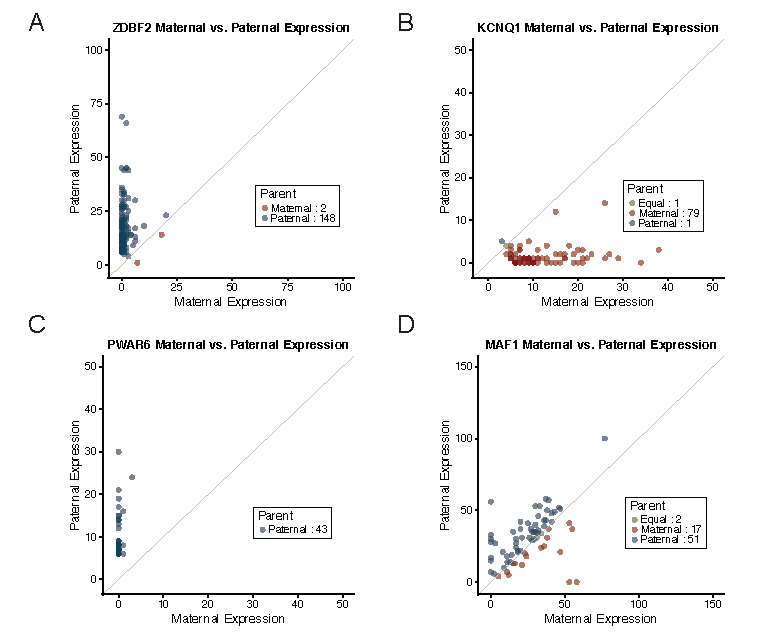
\includegraphics[width=7in]{img/ch03/fig-01}
\caption[Plot of maternal (x-axis) and paternal (y-axis) gene expression for four genes.]{\textbf{Plot of maternal (x-axis) and paternal (y-axis) gene expression for four genes.} Plot of maternal (x-axis) and paternal (y-axis) gene expression for four genes. (A) maternally imprinted gene \emph{ZDBF2} (paternally expressed), (B) paternally imprinted gene \emph{KCNQ1} (maternally expressed), (C) novel maternally imprinted gene \emph{PWAR6} (paternally expressed), (D) gene with asymmetry in parental expression \emph{MAF1}. Each point represents one individual. Numbers in the legend represent the number of individuals with equal maternal and paternal expression, more maternal expression, or more paternal expression.}
\label{fig:matpatexpression}
\end{figure}


Two genes showed gene expression signatures consistent with imprinting but have not previously been recognized as imprinted genes. The first potentially novel imprinted gene is \emph{PXDC1}, which is in the same region and next to (<100kb) a known imprinted gene, \emph{FAM50B}. The second potentially novel imprinted gene is \emph{PWAR6}, or Prader Willi Angelman Region RNA6, a gene encoding regulatory class of RNA. Although this gene is located within the intron of a known imprinted region, \emph{SNHG14}, this noncoding RNA has not previously been recognized as having parent of origin specific expression (Fig 1C).

The remaining fifteen genes show significant asymmetry using the binomial test but do not have expression from mostly one parental chromosome. One of these genes, \emph{SNHG17}, is a noncoding RNA. Another gene with parent of origin asymmetry,  \emph{ZNF813}, is next to a known imprinted gene, \emph{ZNF331}. The remaining genes with asymmetrical parent origin expression have almost equal expression on both parental chromosomes. These genes include  \emph{DAAM1},  which is involved in cytoskeleton, specifically filopodia formation \citep{Hoffmann:2014ki, Luo:2016db}, and has a suggested role for cytoskeleton organization during Mammalian testis morphogenesis and gamete progression \citep{Pariante:2016kn};  \emph{RP11-379H18.1}, a noncoding RNA gene;  \emph{HMGN1P38} \citep{StrichmanAlmashanu:2003cw}; MTX2, a nuclear gene that interacts with mitochondrial membrane protein metaxin 1 and is involved in mitochondrial protein import and metabolism of proteins in mice;   \emph{MAF1} a negative regulator of RNA polymerase 2;  \emph{ZNF714},  \emph{CPNE1},  \emph{IL16},  \emph{ATP6V0D1},  \emph{FAHD1},  \emph{HSP90AB3P}, and  \emph{CNN2} are the remaining genes that show parent of origin asymmetry but not with a pattern consistent with imprinting (S1 Figure).

\subsection{Validation of Imprinted Genes in PBLs}\label{Validation of Imprinted Genes in PBLs}
Using the same methods described above, we assigned parent of origin to transcripts in PBLs from 99 Hutterite individuals not included in the LCL studies. Maternal and paternal expression in PBLs for all 28 genes identified in LCLs showed similar trends of asymmetry as in LCLs (Figure 2). 


\begin{figure}[!htb]
\centering 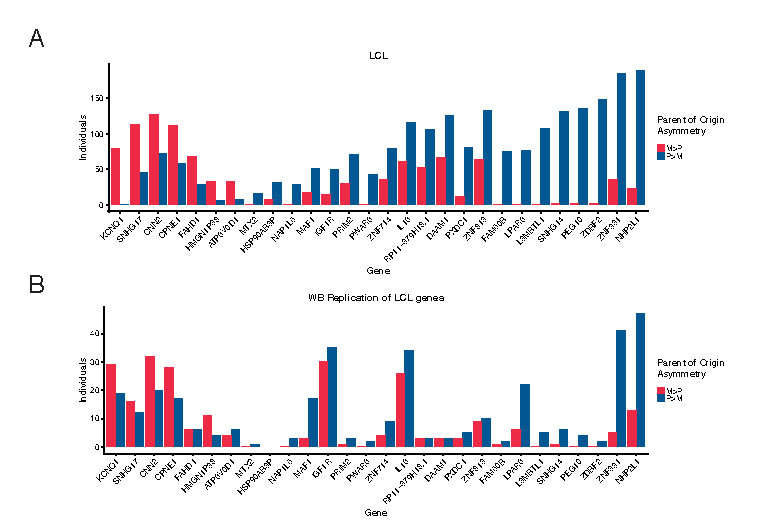
\includegraphics[width=6in]{img/ch03/fig-02}
\caption[Validation in PBLs]{\textbf{Validation in PBLs}Histogram showing the number of individuals with more maternal expression (M>P) or more paternal expression (P>M) for the 28 genes showing parent of origin asymmetry in LCLs (A) and PBLs (B) Genes are ordered by the magnitude of the difference in the number of individuals with more maternal expression than paternal expression in LCLs. }
\label{fig:matpatPBLs}
\end{figure}


\subsection{Methylation at Imprinting Control Regions}\label{Methylation at Imprinting Control Regions}
One of the mechanisms underlying parent of origin effects on expression at imprinted loci is differential methylation at cis-acting imprinting control regions (ICRs). DNA methylation from the Illumina HumanMethylation 450K array was available in PBLs from the same individuals included in the validation studies described above. To determine the expected patterns of methylation at known imprinted loci, we first looked at previously characterized methylated regions at known imprinted regions from Court et al. and Joshi et al. \cite{Court:2014kc,Joshi:2016bb}.

The methylation patterns at the two potentially novel imprinted genes identified in this study, \emph{PXDC1} and \emph{PWAR6}, lie in or near known imprinted regions that contain previously characterized ICRs. Previously characterized ICRs near show about 50\% methylation (beta value of between 0.25 and 0.75) in our DNA methylation data, which likely reflect methylation at only one parental chromosome in all the cells in the sample. Methylation patterns in PBLs at these two ICRs fall within this hemi-methylation range, further suggesting that these two genes are indeed imprinted (Fig 3).


\begin{figure}[!htb]
\centering 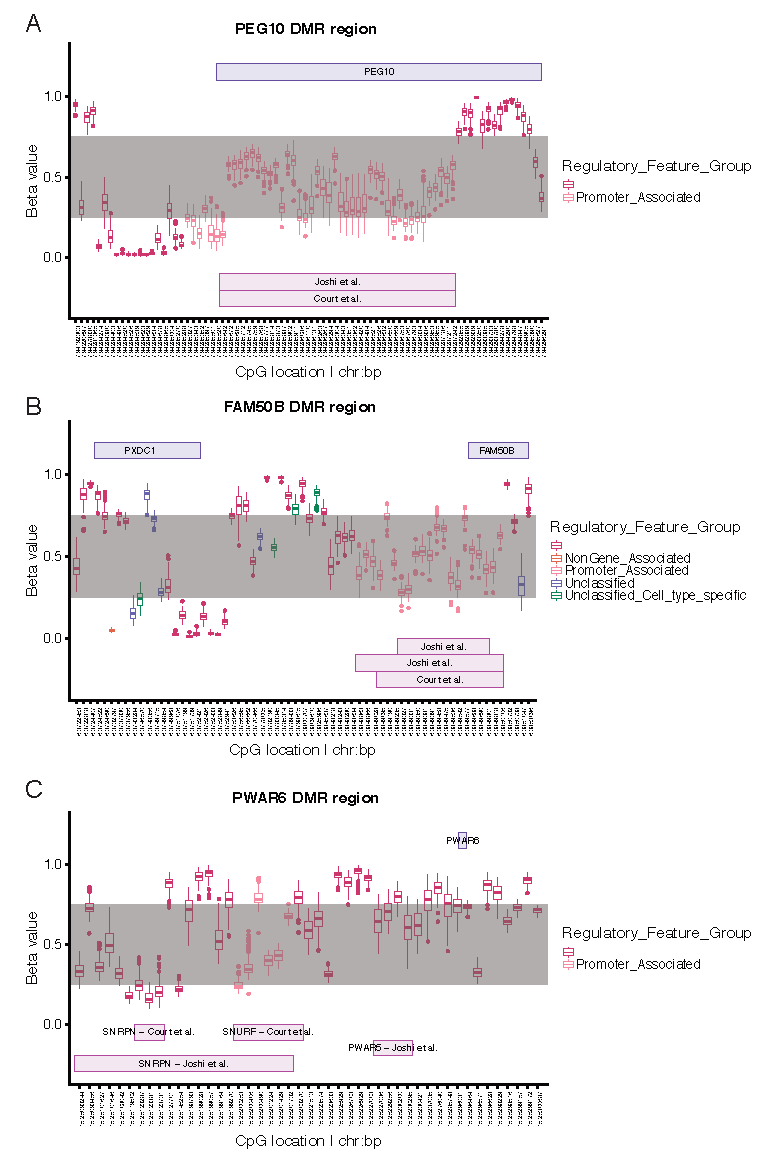
\includegraphics[width=5in]{img/ch03/fig-03}
\caption[Methylation at ICRs]{\textbf{Methylation at ICRs} DNA methylation levels near known and novel imprinted genes previously defined by Joshi et al. and Court et al. (A) \emph{PEG10}, (B) \emph{PXDC1} and \emph{FAM50B}, (C) \emph{PWAR6}.}
\label{fig:methylation}
\end{figure}


\section{Discussion}\label{ch03-discussion}
Dysregulation of imprinted genes can have a large impact on mammalian development and has been associated with significant diseases in humans. Studies aimed at identifying imprinted genes at genome-wide levels have used allele specific expression and imbalance to infer parent of origin. Here we used a large pedigree with assigned parent of origin alleles to map transcripts to chromosomes with known parent of origin and identify imprinted genes. 

Using this approach, we found genes with expression primarily from either the maternal or paternal haplotype. Because gene silencing at imprinted loci may be incomplete, we used a binomial test on parent of origin gene expression and identified 11 known imprinted genes and two potentially novel imprinted genes. Both of these novel genes, PWAR6 and PXDC1, lie in known imprinted regions but have not themselves been characterized as imprinted. The remaining genes that have significant parent of origin asymmetry in gene expression do not show clear imprinting expression patterns. To validate these findings, we mapped gene expression in PBLs from Hutterite individuals not included in the LCL study. The same genes showed similar patterns of asymmetry in these different cell sources (transformed B cells and peripheral blood leukocytes) from different individuals.

In addition to validating gene expression, we characterized methylation patterns near genes showing asymmetry. Using results from studies that had previously characterized ICRs in patients with uniparental disomy at many imprinted regions \citep{Joshi:2016bb, Court:2014kc}, we estimated regions for defining hemi-methylation near the genes identified in our study. Using this approach, we were able to provide additional supportive data for the two potentially novel imprinted genes to be true imprinted genes regulated by previously characterized ICRs. 

Although our study is the largest pedigree-based study to date to search genome-wide for imprinted genes, it has limitations. First, we are able to determine the parent of origin for many transcripts in the Hutterites but we could not assign every RNA sequencing read to a parent due to lack of heterozygous sites or missing parent of origin information for alleles. Second, we conducted these studies in lymphoblastoid cell lines, and therefore could only study genes imprinted in this cell type and would miss the many imprinted genes that are tissue-specific and/or developmentally regulated. Third, while we can verify previously characterized ICRs, our study is not designed to identify novel ICRs because DNA methylation values from an array cannot be assigned to parental haplotype. Lastly, although we characterized the gene expression and methylation patterns for two potentially novel imprinted genes, replication of these genes in a different population and in different tissues, and functional characterization of these genes are required to confirm their status as imprinted genes. Similarly, some of the other genes with parent of origin asymmetry in the blood cells examined in this study may show more clear-cut evidence for imprinting in other tissues or at specific periods of development.  

In summary, we have identified novel imprinted genes using gene expression from a founder population. The genes with asymmetrical parental expression had similar patterns of asymmetry in a different source of blood cells and in different individuals, and we were able to replicate the methylation patterns in known ICRs near the known and novel imprinted genes in this study. Our method and study population allowed us to map reads to parental haplotypes and uncovered \emph{PWAR6} and \emph{PXDC1} as novel imprinted genes that could potentially impact disease risk and development.

\section{Methods}\label{ch03-methods}

\subsection{Genotypes}\label{Genotypes}
Hutterite individuals (n=1,653) were genotyped using one of three Affymetrix genotype arrays, as previously described\citep{Livne2015}, of which 121 underwent whole genome sequencing by Complete Genomics, Inc (CGI) (n=98) or Illumina whole genome sequencing (n=27). A total of 10,235,233 variants present in the sequenced individuals were imputed and phased to the remaining 1532 genotyped individuals using PRIMAL\citep{Livne2015}. Parent of origin was assigned to 89.85\% of the alleles with call rate 81.6842\% after QC. For this study, we included individuals with genotyped parents in the primary analyses in LCLs. Written consents for these studies were obtained from the adult participants and parents of children under 18; written assents were obtained from all children. This study was approved by the University of Chicago Institutional Review Board.   

\subsection{RNA-seq in Lymphoblastoid Cell Lines (LCLs).}\label{RNA-seq in Lymphoblastoid Cell Lines (LCLs).}
RNA-seq was performed in LCLs as previously described \citep{Cusanovich:2016id}. For this study, sequencing reads were reprocessed as follows. Reads were trimmed for adaptors using Cutadapt (reads less than 5 bp discarded) then remapped to hg19 using STAR indexed with gencode version 19 gene annotations\citep{Dobin:2002by, Martin:2011eu}. To remove mapping bias, reads were processed and duplicate reads removed using WASP \citep{vandeGeijn:2015hi}. We used a custom script modified from WASP to separate reads that overlap maternal alleles or paternal alleles. Reads without informative SNPs (homozygous, or no parent of origin information) were categorized as unknown where the unknown, maternal, and paternal make up the total gene expression. Gene counts were quantified using STAR for each category. VerifyBamID was used to identify sample swaps \citep{Jun:2012je}. Genes mapping to the X and Y chromosome were removed; genes with a CPM log transformed value less than 1 in less than 20 individuals were also removed.

\subsection{RNA-seq in Peripheral Blood Leukocytes (PBLs) }\label{RNA-seq in Peripheral Blood Leukocytes (PBLs) }
RNA-seq was performed in whole blood as previously described \citep{Stein:2016hn}. For this study, sequencing reads were reprocessed as described above for the studies in LCLs. For all analyses, we excluded 32 individuals who were also in the LCL study.

\subsection{Identifying Imprinted Genes}\label{Identifying Imprinted Genes}
We used a binomial test to detect asymmetry in parent of origin gene expression. We generated a binomial Z-score for each individual for each gene ($Z_i$) and excluded those where $Z_i =0$. For each gene, the number of subjects with $Z_i >0$ can be modeled by a Binomial distribution with probability 1/2. For imprinted genes that show patterns of asymmetry, we expect a distribution of Z-scores that are skewed to one direction: right-skewed for genes asymmetrically maternally expressed and left-skewed for genes asymmetrically paternally expressed. Because we are only asking whether there are more individuals with more maternal expression or more paternal expression and not gene expression measures there is no need to model over-dispersion.

\subsection{DNA methylation profiling and processing in PBLs}\label{DNA methylation profiling and processing in PBLs}
One milliliter of whole blood from 145 Hutterites was drawn into TruCulture (Myriad RBM; Austin, Texas) tubes containing proprietary TruCulture media. DNA was extracted using AllPrep DNA/RNA Mini Kits (Qiagen). DNA samples were bisulfite converted and hybridized to the Illumina HumanMethylation 450K array at the University of Chicago Functional Genomics Center.  Samples were processed using default parameters using the R package minfi \citep{Aryee:2014by}, normalized using SWAN (subset within-array normalization \citep{Maksimovic:2012ib}) and quantile normalized similar to previous methylation studies \citep{NicodemusJohnson:2016go}.  Probes were removed if: (1) mapped non-uniquely to a bisulfite-converted genome; (2) mapped to sex chromosomes; (3) had a probe detection p-value >0.01 in at least 25\% of samples; and (4) contained common SNPs within the probe sequence, as previously described\citep{Banovich:2014bn}. Principal components analysis (PCA) was used to identify significant technical covariates, and the ComBat function \citep{Johnson:2007fp} within the R package sva \citep{Leek:2012ee} was used to correct for chip effect. Analyses of DNA methylation levels were conducted using beta values, which were converted from M-values using the lumi R package \citep{Du:2008ev}.















% Chapter 04
% Chapter 04
\chapter{Parent of Origin Effects on Gene Expression }\label{ch:poeqtl}
\section[Abstract]{Abstract}

In this chapter, I explore the impact of parental origin of genetic variation on gene expression. 


\section{Introduction}\label{ch04-introduction}

For example, Garg et al. used gene expression in LCLs from HapMap trios to identify 30 imprinting eQTLs with parent of origin specific effects on expression including two imprinted genes\cite{Garg2012a}

\section{Results}\label{ch04-results}
\subsection{Opposite Parent of Origin eQTL}\label{Opposite Parent of Origin eQTL} 
Our opposite parent of origin eQTL did not find any significant results (Bonferonni corrected p-value). We were originally going to follow up significant results from this analysis with maternal and paternal eQTLs using maternal and paternal expression, respectively. 

\subsection{Single Parent eQTL}\label{Single Parent eQTL} 
We performed the maternal and paternal eQTL analysis anyway, first using parent of origin normalized expression as well as normalized parental expression with uninformative genes removed. We had to remove uninformative genes, as described in the Methods, since the data was sparse and zeros drove most of the analysis.  (Figure xx). 

There were xx SNP gene pairs we could compare across both single parent eQTLs. For those significant in one or the other, the effect sizes were all in the same direction, where we were hoping some SNPs could have opposite effects on their corresponding parental gene expression (Figure xx).

We then compared SNP gene pairs that were significant (Bonferroni) in one parent, and not significant (p>0.05) in the other parent (7,712 SNP gene pairs maternal significant associations not paternally significant; 10,815 paternal significant associations not maternally significant). 

Unfortunately, these are still driven by sparse data and don't look like real parent of origin effect eQTLs (Figure xx).

\subsection{Modified ASE Test}\label{Modified ASE Test} 

For a more simple approach, we did a simple $\chi^2$ test on the reciprocal heterozygotes on their corresponding maternal and paternal expression using maternal and paternal count data corresponding to haplotype specific expression. 
Using Bonferroni corrected p-value we identified xx significant results. 


\section{Discussion}\label{ch04-discussion}



\section{Methods}\label{ch04-methods}

\subsection{Genotypes and Sample Information}\label{Genotypes and Sample Information}
LCL RNA-seq transcripts for 306 individuals were mapped to parental haplotypes as in Chapter \ref{ch:imprinted}. We used the measures of total as well as maternal and paternal expression in this study. We used multiple approaches to characterize parent of origin effects on gene expression.
To be conservative, we used 306 Hutterite individuals for which we have parental genotypes and tested SNPs for which we have at least three individuals in at least three of four parent of origin genotype classes (such that we have at least three individuals in at least one heterozygote category and one heterozygote individual will not drive our analysis).

\subsection{RNA-seq QC}\label{RNA-seq QC}
Multiple approaches required different QC method. For the total gene expression, we used normalized gene expression. First, we removed lowly expressed genes with a log count per million (cpm) greater than 1 in at least 20 individuals.The R/Bioconductor package edgeR was used to convert the RNA-seq counts to log2 TMM-normalized CPM values\cite{Robinson:2010dd,Robinson:2010cw}. Technical covariates correlated with gene expression Principal Components were regressed out (xx, xx, xx, xx). 

Maternal gene expression was used as both counts and as normalized gene expression. Maternal gene expression counts were used directly from STAR gene count output\cite{Dobin:2002by} subsetted on genes included in the total gene expression analysis. 
Normalized maternal expression was calculated using similar to total gene expression using edgeR and converting RNA-seq counts to log2 TMM normalized CPM values using normalization factors (library sizes) from the total gene expression (maternal gene expression too sparse on it's own). 
Same method was used to get paternal gene expression counts and normalized paternal gene expression.

To separate informative parental gene expression from uninformative parental gene expression I compiled all of the heterozygous SNPs for each individual for each gene that was expressed. If a gene for an individual did not have any heterozygous parent of origin SNPs (i.e. informative SNPs), the gene was considered missing (converted to NA for downstream analysis). If there was at least one heterozygous parent of origin SNPs in the corresponding gene, the gene expression value was not altered, since zero expression for that gene for that parent could be informative. This nulled different numbers of genes for different individuals. Figure xx


\subsection{Opposite Parent of Origin eQTL}\label{Opposite Parent of Origin eQTL}
We used the same method outlined in Chapter \ref{ch:pogwas} to detect if SNPs had opposite effects on total gene expression by parental origin. 

\subsection{Single Parent eQTL}\label{Single Parent eQTL}
To use the parent of origin expression, we performed an eQTL testing for specific parental effects on the same parental gene expression as follows. 

\begin{equation}
Y _{M}=W\alpha + X_{M}\beta_{M}+g+\epsilon
\end{equation}

\begin{equation}
Y _{P}=W\alpha + X_{P}\beta_{P}+g+\epsilon
\end{equation}








% Chapter 05 - Conclusion
% !TEX encoding = UTF-8 Unicode
\chapter{Conclusion}

As we look past the "low hanging fruit" of GWAS, we turn to other biological mechanisms where genetics can influence our traits, including studies or rare variation\cite{Igartua:2017ir}, gene by environment interactions, and parent of origin effects among others. The Hutterites that the Ober Lab studies are an ideal population to look for parent of origin effects on quantitative disease related traits and gene expression\cite{Weiss:2005cq,Abney2001,Ober:2001dy}. With RNA-seq and novel methods for imputing and phasing data at a population scale\citep{Livne2015}, we are able to start getting at these questions. 

\section{A novel method to detect opposite effects of parentally inherited variants on cardiovascular disease and asthma associated traits}
 
 In Chapter \ref{ch:pogwas}, I described...  background
 
 
 Previous  studies.. 
 
 This novel study
 
main takeaway

future studies
 
\section{Identifying two novel imprinted genes in known imprinted regions using parent of origin gene expression}

% Format a LaTeX bibliography
\makebibliography

% Figures and tables, if you decide to leave them to the end
%\input{figure}
%\input{table}

\end{document}


